\documentclass[12pt]{extarticle}
% \usepackage{fullpage} % for margin adjustment
\usepackage[margin=1in,bottom=1in, top=1in]{geometry}
\usepackage[utf8]{inputenc}
\usepackage{amsmath, amsfonts, amssymb, amsthm}
\usepackage{xcolor} % for text coloring
\usepackage{float}
\usepackage{centernot}
\usepackage{graphicx}
\usepackage{setspace}
%\usepackage{lineno}
\usepackage{subcaption}
\usepackage{wrapfig}
\usepackage{xurl}
\usepackage{tikz}

\usepackage{hyperref}
\usepackage[capitalize]{cleveref}

% import biblatex with prefered settings
% % below are Alex's biblatex settings for the FST paper
%% loads biblatex with all the nice standard options that John determined some time ago!
%% this version uses a ``Harvard'' style (first author last name, year in parentheses).
%% also loads xpatch

%% biblatex
%% harvard style
\usepackage[style=authoryear,natbib,maxcitenames=2,doi=false,isbn=false,url=false,backend=bibtex,date=year,giveninits=true,uniquename=init]{biblatex}
%% numeric style
%%% \usepackage[style=numeric-comp,sorting=none,giveninits=true,
%%%                      doi=false,isbn=false,url=false,backend=bibtex,date=year]{biblatex}
%% remove "In: " before journal title
\renewbibmacro{in:}{}
%% remove language
\AtEveryBibitem{\clearlist{language}}
%% remove month
%%\AtEveryBibitem{\clearfield{month}}
%% remove dots between volume and issue
\usepackage{xpatch}
\xpatchbibmacro{volume+number+eid}{%
  \setunit*{\adddot}%
}{%
}{}{}
%% put issue in parentheses
\DeclareFieldFormat[article]{number}{\mkbibparens{#1}}
\DeclareFieldFormat[article]{citetitle}{#1}
\DeclareFieldFormat[article]{title}{#1}

% below are Alex's biblatex settings for the FST paper
%% loads biblatex with all the nice standard options that John determined some time ago!
%% this version uses a ``Harvard'' style (first author last name, year in parentheses).
%% also loads xpatch

%% biblatex
%% harvard style
%%% \usepackage[style=authoryear,natbib,maxcitenames=2,doi=false,isbn=false,url=false,backend=bibtex,date=year]{biblatex}
%% numeric style
\usepackage[style=numeric-comp,sorting=none,doi=false,isbn=false,url=false,backend=bibtex,date=year]{biblatex}

%% to have citep etc work without a hitch here...
\newcommand{\citep}{\cite}
\newcommand{\citet}{\cite}

%% remove "In: " before journal title
\renewbibmacro{in:}{}
%% remove language
\AtEveryBibitem{\clearlist{language}}
%% remove month
%%\AtEveryBibitem{\clearfield{month}}
%% remove dots between volume and issue
\usepackage{xpatch}
\xpatchbibmacro{volume+number+eid}{%
  \setunit*{\adddot}%
}{%
}{}{}
%% put issue in parentheses
\DeclareFieldFormat[article]{number}{\mkbibparens{#1}}


\bibliography{causaltrio-refs}

\newtheorem{asm}{Assumption}%[section]
\newtheorem{clm}{Claim}%[section]
\newtheorem{thm}{Theorem}%[section]
\newtheorem{lem}{Lemma}%[section]
\newtheorem{defin}{Definition}%[section]
\newtheorem{exm}{Example}%[section]

\newcommand\scalemath[2]{\scalebox{#1}{\mbox{\ensuremath{\displaystyle #2}}}}
\newcommand{\ind}{\perp\!\!\!\!\perp}
\newcommand{\inte}{\mathrm{int}}
\newcommand{\iid}{\stackrel{\text{iid}}{\sim}}
\newcommand{\eqe}{\stackrel{\cdot}{=}}
\newcommand{\ascon}{\underset{J\to \infty}{\overset{a.s.}{\longrightarrow}}}
\newcommand{\pcon}{\stackrel{P}{\longrightarrow}}
\newcommand{\dcon}{\stackrel{D}{\longrightarrow}}
\newcommand{\pp}{\mathbb{P}}
\newcommand{\E}{\mathbb{E}}
\newcommand{\Y}{Y^{\ast}}
\newcommand{\nind}{J}
\newcommand{\nsnp}{I}
\newcommand{\indicator}{\mathcal{I}}
\newcommand{\intercept}{\iota}
\newcommand{\ace}{{\normalfont \text{ACE}}}
\newcommand{\are}{{\normalfont \text{ARE}}}
\newcommand{\tmt}{{\normalfont \text{TMT}}}
\newcommand{\tdt}{{\normalfont \text{TDT}}}
\newcommand{\dtmtnc}{d_{\tmt}^{\normalfont \text{nc}}}
\newcommand{\dtmtpc}{d_{\tmt}^{\normalfont \text{pc}}}
\newcommand{\vir}{\sigma^2_{\text{pc,1}}}
\newcommand{\virb}{\sigma^2_{\text{pc,2}}}
\newcommand{\virc}{\sigma^2_{\text{pc,3}}}
\newcommand{\vtmthat}{\hat{\sigma}^2_{\text{TMT}}}
\newcommand{\dir}{d_{\text{IR}}}

\newcommand\tablefontsize{\fontsize{12pt}{14pt}\selectfont}
\newcommand\tocfontsize{\fontsize{12pt}{14pt}\selectfont}
\renewcommand*{\thepage}{\footnotesize\arabic{page}}

\newcommand{\bZ}{\boldsymbol{Z}}
\newcommand{\V}{\mathbb{V}}
\newcommand{\cV}{\mathbb{C}}
\newcommand{\cC}{\mathcal{C}}
\newcommand{\cH}{\mathcal{H}}
\newcommand{\cU}{\mathcal{U}}
\newcommand{\cJ}{\mathcal{J}}
\newcommand{\cT}{\mathcal{T}}

\usetikzlibrary{arrows}
\usetikzlibrary{shapes}
\newcommand*\circled[1]{\tikz[baseline=(char.base)]{
            \node[shape=circle,draw,inner sep=2pt] (char) {#1};}}

%\setlength{\marginparwidth}{2cm}


\renewcommand{\baselinestretch}{1.3}\selectfont

\begin{document}

% \onehalfspacing

\thispagestyle{empty}

\noindent {\Large \textbf{Identifying causal genotype-phenotype relationships for population-sampled parent-child trios}}

\vspace{6pt}

\noindent Yushi Tang$^{\ast}$, Irineo Cabreros$^{\dag}$, and John D. Storey$^{\ast, 1}$

\vspace{6pt}
\noindent $^{\ast}$Lewis-Sigler Institute for Integrative Genomics and $^{\dag}$Program in Applied and Computational Mathematics, Princeton University, NJ 08544, USA


\noindent $^{1}$Corresponding author: \texttt{jstorey@princeton.edu}


\vspace{6pt}
\noindent \textbf{Abstract:} The process by which genes are transmitted from parent to child provides a source of randomization preceding all other factors that may causally influence any particular child phenotype. Because of this, it is natural to consider genetic transmission as a source of experimental randomization. In this work, we show how parent-child trio data can be leveraged to identify causal genetic loci by modeling the randomization during genetic transmission. We develop a new test, the transmission mean test (TMT), together with its unbiased estimator of the average causal effect, and derive its causal properties within the potential outcomes framework. We also prove that the transmission disequilibrium test (TDT) is a test of causality as a complementary case of the TMT for the affected-only design. The TMT and the TDT differ in the types of traits that they can handle and the study designs for which they are appropriate. The TMT handles arbitrarily distributed traits and is appropriate when trios are randomly sampled; the TDT handles dichotomous traits and is appropriate when sampling is based on a child's trait status. We compare the transmission-based methods with established approaches for genotype-phenotype analyses to clarify conditions appropriate for each method, what conclusions can be drawn by each one, and how these methods can be used together.   

\vspace{6pt}
\noindent \textbf{Keywords:} causal inference, causal linkage, genome-wide associations, potential outcomes, randomized experiments, transmission disequilibrium, transmission mean test

\clearpage

\thispagestyle{empty}

\tableofcontents
%\begin{singlespace}
%{\tocfontsize \tableofcontents}
%\end{singlespace}

\clearpage

\pagenumbering{arabic}
\setcounter{page}{1}

%\linenumbers

%\setlength{\abovedisplayskip}{-6pt}

\section{Introduction}\label{sec:intro}

The ultimate goal of understanding the genotype-phenotype relationship is to uncover genetic variants that are causal for the phenotype. The gold standard statistical framework for establishing causality is the potential outcomes framework \citep{neyman1923, rubin1974, imbens2015}. This paper investigates how human trio data (two parents and their child) can enable tests of causality based on comparisons of trait level potential outcomes corresponding to different alleles transmitted from the parents to the child. The motivation lies in the connection between the meiotic process and experimental randomization. The biological process of meiosis is inherently random, ensuring that multiple children from a single pair of parents have independent variation in their inherited genetics. Since the variation induced by meiosis precedes other events that may influence a particular trait and it is randomized within a trio, meiosis resembles a form of experimental randomization. This was recognized early in the development of genetics, such as in Fisher's 1951 lecture \citep{fisher1952}:

\begin{quote}
``The different genotypes possible from the same mating have been beautifully randomised by the meiotic process. A more perfect control of conditions is scarcely possible, than that of different genotypes appearing in the same litter."
\end{quote}

\noindent In a properly randomized experiment, it is a basic result that association implies causation \citep{rubin1974, holland1986, greenland1990}. If one accepts meiosis as a valid form of experimental randomization, then genotypes associated with a phenotype can be interpreted causally by leveraging the randomization of alleles transmitted during meiosis.

Fisher's observation that the meiotic process is a valid form of randomization is essentially correct within the single family or litter setting. However, when analyzing population-sampled trios that consist of multiple families, the analogy between a randomized experiment and meiosis does not trivially extend to the collection of families analyzed together. For instance, in a sampled population, there may be confounding between genetic variation and a trait. One reason for this is \textit{population structure}, commonly observed in human populations \citep{hao2019}. In a population, the processes that gave rise to genetic variation may be related to the processes that influence a trait. 

Even though a phenotype cannot, in principle, change a genotype and even though genotypes are \textit{randomly sampled}, this does not mean that population-based studies in general contain the information needed to leverage the randomization due to meiosis. A related but distinct line of work, referred to as ``Mendelian randomization'' (MR), aims to identify non-genetic factors that are causal for phenotypes of interest. The challenges and underlying assumptions of MR have been variously discussed \citep{smith2004, nitsch2006, bochud2008}. MR constructs instrumental variables from genotypes for population-sampled individuals but does not directly observe the meiotic process from parents to child. It is not a potential outcomes framework applied to trios where randomization is directly observed, as we consider here. 

The current state of understanding is that other than in the single-family setting, therefore, association implies neither causation nor proximity to causal loci, which is why association studies are not considered to be linkage or causality studies. Genome-wide association studies (GWAS) determine statistical associations between genotypes and phenotypes without any general proof of causality. A framework has been proposed for causal inference where the parents and child have phased genomes available \citep{bates2020}. This framework utilizes a definition of causality based on probabilistic independence \citep{pearl2009}, which is not necessarily equivalent to the potential outcomes we employ here \citep{imbens2015}. % The method assumes independent crossovers during meiosis \citep{lange2002}, which may not hold in humans \citep{myers2005, coop2008, kivikoski2023}. The framework requires a computationally intensive simulation-based null distribution. 

Here we develop a robust randomization-based causal framework for genotype-phenotype relationships by considering two \textit{transmission-based methods} --- one introduced here for arbitrarily distributed phenotypes in population-sampled trios and the other for an existing method applied to dichotomous traits in a particular type of trio study. These methods do not require phased genomes, but rather standard diploid genotypes for parents and child. We name the first approach the \textit{transmission mean test} (TMT) and refer to the second approach under its known name, the \textit{transmission disequilibrium test} (TDT). The TMT is a new set of methodologies developed here for both quantitative (continuous or counts) and binary phenotypes, when trios are randomly sampled from an arbitrarily structured population with other potential genotype-phenotype confounders. Such study designs occur, for example, when trios are sampled from a defined geographical region \citep{pcgc2013, bycroft2018, allofus2024} or from a particular population \citep{pollin2004, goring2007}, or when trios are sampled on the basis of parent-level attributes \citep{lee2014}. The TDT handles trios that have an ``affected'' child of a binary phenotype. Previous work described the study design for the TDT as \textit{affected-only design}, also known as \textit{affected family-based controls}, and have developed the TDT as a statistical test of association \citep{thomson1988, terwilliger1992, spielman1993, ewens1995, allison1997, laird2000, laird2006}. We show here that the TDT is a rigorous test of causality. 

The main contributions of this work are to propose the TMT and to establish that the TMT and the TDT are valid causal inference methods within the potential outcomes framework. We start by assuming that the causal and non-causal variants are probabilistically independent. We define the concept of \textit{directly causality} and develop the TMT to detect causal genetic effects for a broad class of traits. We prove that the TDT is a causal test for dichotomous traits in the affected-only design. We then extend the causal framework of both the TMT and the TDT to the case where causal and non-causal loci may be genetically linked by developing the concept of \textit{causal linkage}. In order to identify scenarios appropriate for these methods and how they can be used together with existing methods, we compare the proposed causal inference framework with established association methods, such as the linear mixed model for associations (LMM) \citep{kang2010,yang2010,yang2011}, in the presence of population structure and confounding factors associated with both the trait and causal genotypes.

\section{Theory and Methods}\label{sec:tmt_concept}

\subsection{Data structure and method overview} \label{sec:tmt_basic_aims}

\paragraph{Trio data.} The data for an observed trio includes the child's measured phenotype as well as the genome-wide genotypes of both parents and the child (\Cref{fig:randomization}). The goal here is to identify the genetic loci that are causal for the measured phenotype among the children. Let $\nind$ be the total number of trios. A sample of $\nind$ trios will involve $3\nind$ distinct individuals. We assume that no individual is the parent of more than one child in the sample and no individual appears both as a parent and as a child in the sample. 

Our framework starts from the unphased biallelic \textit{single nucleotide polymorphism} (SNP) data \citep{williams1990}, which is more common than phased data in practical settings. Let $\nsnp$ be the total number of SNPs per individual. For a SNP, let $a$ and $b$ be the two alleles that generate three possible genotypes $\{aa,ab,bb\}$. We numerically encode these three genotypes by $\{0,1,2\}$. In the $j$th trio, $j\in [1:\nind]$, let $G_{ij}\in \{0,1,2\}$ be the child's $i$th genotype, $Z_{ij}^m\in \{0,1,2\}$ the maternal $i$th genotype, and $Z_{ij}^p\in \{0,1,2\}$ the paternal $i$th genotype, $i\in [1:\nsnp]$. A complete set of trio genotype data includes the $\nsnp \times \nind$ matrix $\boldsymbol{G}=\{G_{ij}\}$ for the child and $\nsnp \times \nind$ matrices $\boldsymbol{Z}^m=\{Z_{ij}^m\}$ and $\boldsymbol{Z}^p=\{Z_{ij}^p\}$ for the parents. 

We additionally denote $G_{ij}=A_{ij}^m+A_{ij}^p$ for each child, where $A_{ij}^m\in \{0,1\}$ is the allele the $j$th child received from the maternal side and $A_{ij}^p\in \{0,1\}$ the allele from the paternal side. We do not assume that the parental transmitted alleles $\boldsymbol{A}^m=\{A_{ij}^m\}$ and $\boldsymbol{A}^p=\{A_{ij}^p\}$ are directly observed in our framework. In addition to the genotype data, we observe a $\nind$-length vector of child's phenotypes $\boldsymbol{Y}=\{Y_j\}$ where $Y_j$ can be either quantitative (continuous or counts) or dichotomous. % The complete set of notation is summarized in \Cref{tab:term}. 
Let $\cC$ be the index set of causal SNP(s) for a specific trait $Y$. The goal is to identify all $i\in \cC$ such that there exists a causal effect from $G_i$ to $Y$. As $G_i=A_i^m+A_i^p$ and we are not distinguishing maternal and paternal genetic effects, an equivalent aim is to estimate the causal effect from $(A_i^m,A_i^p)$ to $Y$. 

\paragraph{Overview of the proposed framework.} \label{sec:tmt_procedure}

\begin{figure}
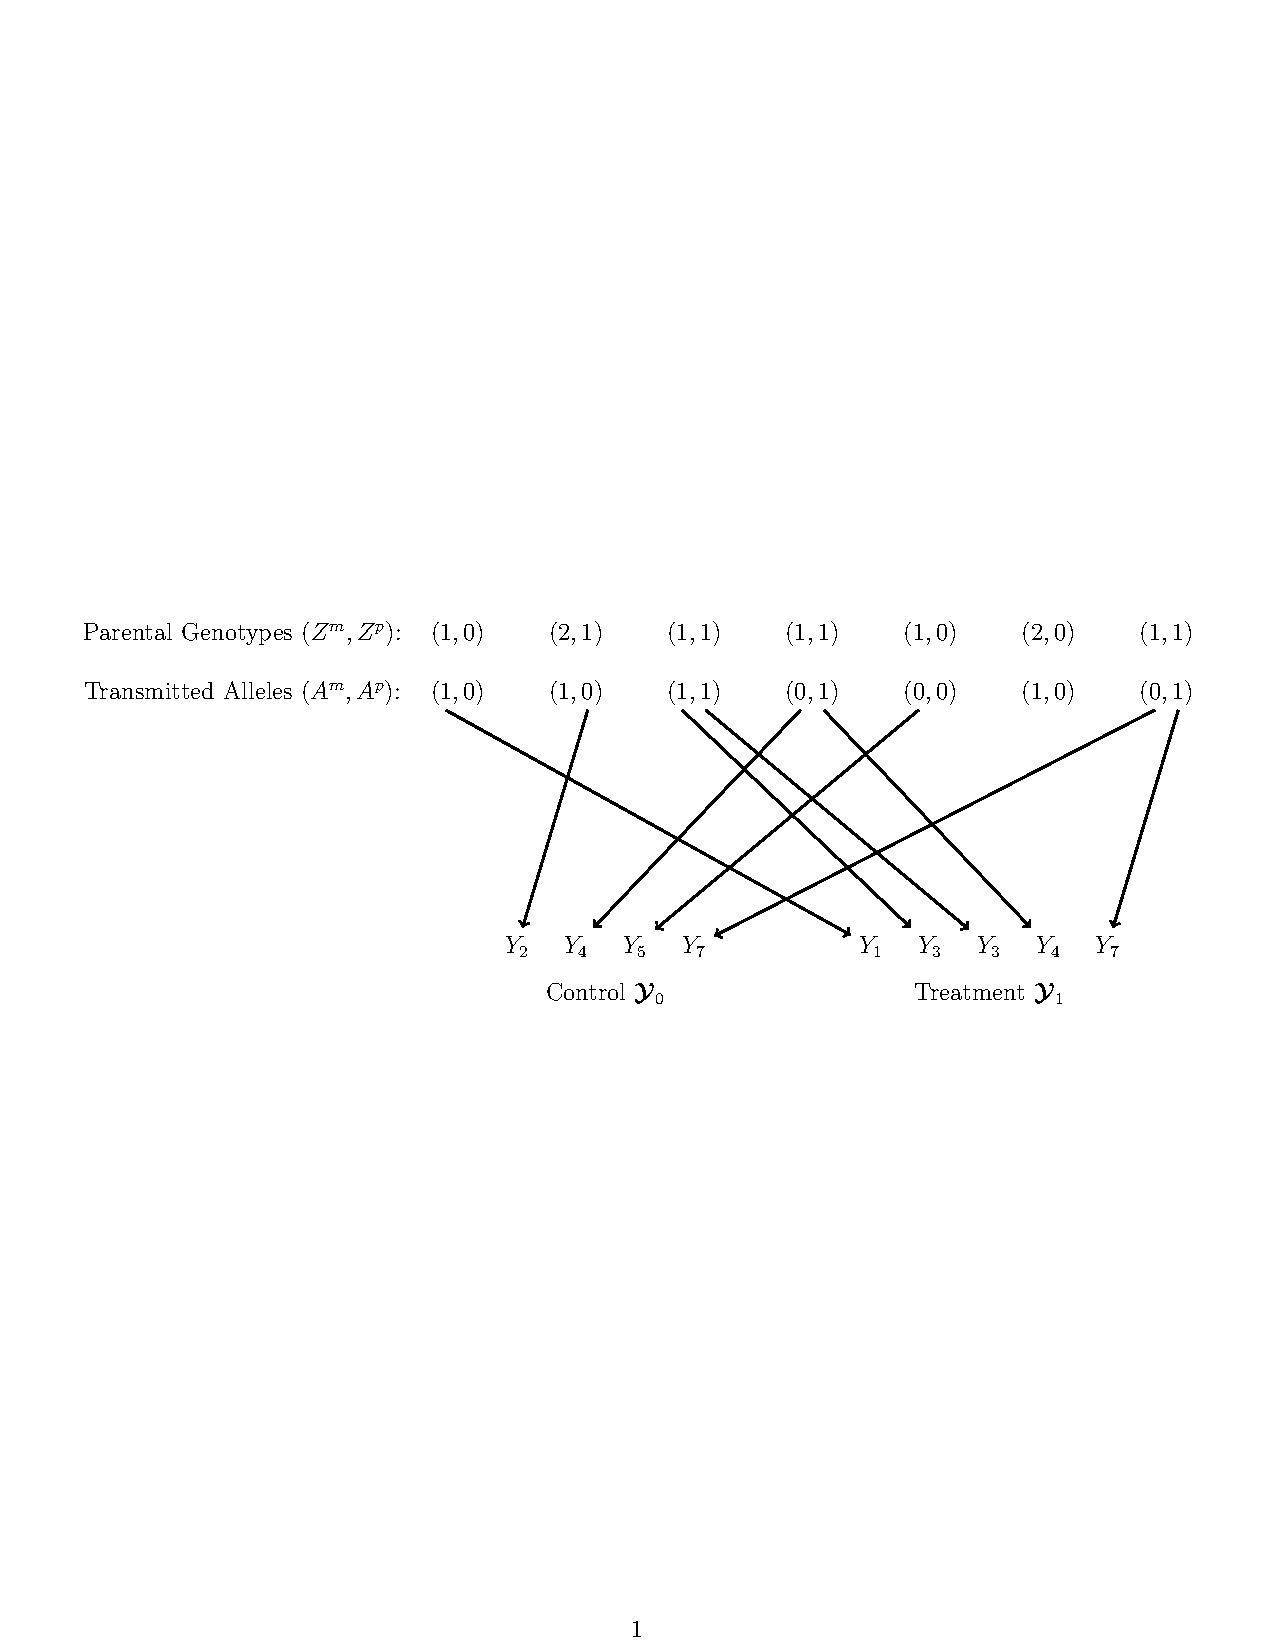
\includegraphics[clip, trim=1.2cm 10.8cm 0cm 9cm, width = 1\textwidth]{./figures/figure1.pdf} % trim by left botm right top
\caption{\textbf{Schematic of the TMT assignment procedure}. Encode the two possible transmitted alleles at the $i$th locus as allele $0$ and $1$. Let $Y$ be the value of the child's phenotype. In the $j$th trio, if a heterozygous parent transmits an allele $0$ to the child, the corresponding phenotype $Y_j$ is included in the control group. If a heterozygous parent transmits an allele $1$, the corresponding $Y_j$ is included in the treatment group. When there are two heterozygous parents, a trait can be included twice within one group or it can be assigned simultaneously to both groups. We do not observe a randomization from a homozygous parent.}
\label{fig:tmt_procedure}
\end{figure}

Here we give a conceptual overview of the proposed \textit{transmission mean test} (TMT).  The main idea is the characterization of the randomizations that have taken place, shown in \Cref{fig:tmt_procedure}. Each child's trait value is potentially subject to two independent \textit{within-trio} randomizations, one from the maternally transmitted allele and one from the paternally transmitted allele. These transmitted alleles, $A^m_i$ and $A^p_i$, can be either 0 or 1. In order for a meaningful randomization to take place, the parent must be heterozygous. For each heterozygous parent, we assign the child to the \textit{control} group if receiving an allele 0 and to the \textit{treatment} group if receiving an allele 1. The control and treatment group labels are arbitrary. It is the between group difference of trait values that we need in order to estimate causal effects. The key algorithm is the assignment procedure that constructs the control and the treatment groups. If a heterozygous parent in the $j$th trio transmits an allele 0 to the child, the corresponding $Y_j$ is included in the control. Conversely, if transmitting an allele 1, $Y_j$ is included in the treatment. It is possible for a trait value to go into both the control and treatment groups (wherein our proposed statistic cancels out the trait value). It is also possible for a trait value to be assigned twice to the control group if both heterozygous parents contribute 0 alleles and likewise for the treatment group, as shown in \Cref{fig:tmt_procedure}. 

Two vectors, $\boldsymbol{\mathcal{Y}}_0$ and $\boldsymbol{\mathcal{Y}}_1$, are generated, representing the observed trait values in the control and the treatment. Both $\boldsymbol{\mathcal{Y}}_0$ and $\boldsymbol{\mathcal{Y}}_1$ contain two types of elements: one attributed to the maternal side and the other attributed to the paternal side, written as  
\begin{align*}
\boldsymbol{\mathcal{Y}}_0^m &=\{Y_j:Z_{j}^m=1,A_{j}^m=0\},\,\,\boldsymbol{\mathcal{Y}}_0^p=\{Y_j:Z_{j}^p=1,A_{j}^p=0\}, \\
\boldsymbol{\mathcal{Y}}_1^m &=\{Y_j:Z_{j}^m=1,A_{j}^m=1\},\,\,\boldsymbol{\mathcal{Y}}_1^p=\{Y_j:Z_{j}^p=1,A_{j}^p=1\},
\end{align*} 
 where $\boldsymbol{\mathcal{Y}}_0=(\boldsymbol{\mathcal{Y}}_0^m,\boldsymbol{\mathcal{Y}}_0^p),\,\,\,\,\, \boldsymbol{\mathcal{Y}}_1=(\boldsymbol{\mathcal{Y}}_1^m,\boldsymbol{\mathcal{Y}}_1^p)$. 

Randomizations, when occurring in concordance with the required assumptions, allow one to straightforwardly infer causality from associations, even in the presence of confounders. This is well known in simple scenarios, such as a study with a single randomized variable that meets all required assumptions. However, the scenario we consider here with trios is non-standard and presents some interesting challenges.  Sampled trios can have zero, one, or two heterozygous parents. A trio with two heterozygous parents allows us to record two randomizations and it does not leave a homozygous parent acting as a potential confounder. However, the randomization of the two parents can be in opposite directions. In the case of one heterozygous parent and one homozygous parent, it should be noted that confounders with genotype (e.g., via population structure or confounding non-genetic variation) can still enter the child's trait value through the homozygous parent since there is no meaningful randomization from that parent. Trios with zero heterozygous parents are not used to infer causality as there are no meaningful randomizations. 

We introduce a trait model and formulate it as general as possible to account for confounders. We then define a specialized potential outcomes model of causal effects, as it is nonstandard to randomly have zero, one, or two of the potential randomized variables manifesting as discernable randomizations. After these model formulations, we construct a causal effect estimand, together with a TMT statistic, based on the differences between the values in $\boldsymbol{\mathcal{Y}}_0$ and $\boldsymbol{\mathcal{Y}}_1$, and we prove several key operating characteristics of them. 

\subsection{Model assumptions and potential outcomes} \label{sec:gma}

Here, we formulate a trait model and a causal effects model for each SNP and child combination. We therefore drop the SNP subscript $i$ and individual subscript $j$ until they are needed. 

\paragraph{The trait model.} The child's trait $Y$ is modeled as: 

\begin{equation} \label{eq:app_gtm}
\begin{aligned}
Y &= \alpha_0\indicator(A^m+A^p=0) + \alpha_1 \indicator(A^m+A^p=1) + \alpha_2 \indicator(A^m+A^p=2) + \gamma \\
&= \alpha_0\indicator(G=0) + \alpha_1 \indicator(G=1) + \alpha_2 \indicator(G=2) + \gamma.
\end{aligned}
\end{equation}
It is the case that $A^m$, $A^p$, $G$, and $\gamma$ are all random variables whereas $\alpha_0$, $\alpha_1$, and $\alpha_2$ are fixed effects. Due to possible relatedness and population structure, the parental genotypes $Z^m$ and $Z^p$ may be arbitrarily dependent random variables, making $A^m$ and $A^p$ dependent. (We show below that some independence results on $A^m$ and $A^p$ hold when conditioning on certain parental genotypes $Z^m$ and $Z^p$.) We assume that $\gamma$ does not interfere with the transmitted allele from heterozygote parents, detailed precisely in \Cref{asm:law_segregation} below. This model is more general than is typically assumed for the popular linear-mixed effects approach to correct for polygenic background and population structure.

One may propose to fit the trait model in \Cref{eq:app_gtm} by a simple linear regression between the child's trait $Y$ and genotypes $G$. In order to obtain an unbiased estimated of $\alpha_0$, $\alpha_1$, and $\alpha_2$, such a regression approach would require \textit{exogeneity}, i.e., $\E[\gamma|G]=0$ or equivalently $\cV(\gamma,G)=0$. However, this is not necessarily satisfied according to the assumptions underlying \Cref{eq:app_gtm}. For example, when there is population structure or dependence among genetic and non-genetic effects, then exogeneity is violated. 

One assumption we make about the trait model is that the genetic effects are either non-decreasing or non-increasing, but we do not assume an additive genetic model. As shown below, this allows us to tractably deal with the fact that there are two potential parental randomizations within each trio. 
\begin{asm}\label{asm:genetic_model}
The conditional expectation of $Y$ given parental transmitted alleles, $\mathbb{E}[Y|A^m, A^p]$, is either a non-decreasing function of $A^m+A^p$ such that
\begin{align*}
\E[Y|A^m=0,A^p=0] &\leq \E[Y|A^m=0,A^p=1] \\
&= \E[Y|A^m=1,A^p=0] \leq \E[Y|A^m=1,A^p=1]. 
\end{align*}
or $\mathbb{E}[Y|A^m, A^p]$ is analogously a non-increasing function of $A^m+A^p$. 
\end{asm}

\noindent Note that under the trait model in \Cref{eq:app_gtm}, if $\E[Y|A^m,A^p]$ is non-decreasing, then $\alpha_0 \leq \alpha_1 \leq \alpha_2$; if $\E[Y|A^m,A^p]$ is non-increasing, then $\alpha_0 \geq \alpha_1 \geq \alpha_2$. Since the alleles are arbitrarily coded as 0 or 1, without loss of generality we let the allele be 1 that yields an non-decrease in $\E[Y|A^m, A^p]$ and 0 otherwise. This is only for mathematical convenience and does not restrict our procedure or theory. 

\paragraph{Potential outcomes.} To study the causal effect of the parental transmitted alleles $(A^m,A^p)$ on the child's phenotype $Y$ in standard potential outcomes parlance, we model potential outcomes as variables representing the phenotype that the child would have developed if receiving a particular allele from the parental side of interest. Let $A$ be the parental transmitted allele. The potential outcomes are $Y(A=0)$ and $Y(A=1)$, sometimes simplified as $Y(1)$ and $Y(0)$. Then the observed trait value $Y$ can be written as a function of the potential outcomes: 
\begin{align*}
Y&=Y(0)\indicator{(A=0)}+Y(1)\indicator{(A=1)}
\end{align*}
where $\indicator(\cdot)$ is the indicator function. Since the meiotic process for the transmission of the allele only happens once for each child, either $Y(0)$ or $Y(1)$ is observed, but not both. When considering a particular parental side, we write $Y^m(0)$ and $Y^m(1)$ for the maternal side and $Y^p(0)$ and $Y^p(1)$ for the paternal side. Under the trait model in \Cref{eq:app_gtm}, the potential outcomes are 
\begin{equation} \label{eq:potentialoutcomes}
\begin{aligned}[c]
Y^m(0) &= \alpha_0\indicator(A^p=0) + \alpha_1\indicator(A^p=1) + \gamma, \\
Y^m(1) &= \alpha_1\indicator(A^p=0) + \alpha_2\indicator(A^p=1) + \gamma, \\
Y^p(0) &= \alpha_0\indicator(A^m=0) + \alpha_1\indicator(A^m=1) + \gamma, \\
Y^p(1) &= \alpha_1\indicator(A^m=0) + \alpha_2\indicator(A^m=1) + \gamma.
\end{aligned}
\end{equation}

%The potential outcomes above further distinguish our framework from a regression approach. A regression model generally requires independent observations, which does not agree with the potential outcomes above. 

%The potential outcomes for the $j$th child, $(Y^m_j(0), Y^m_j(1), Y^p_j(0), Y^p_j(1))$, are functions of parental transmitted alleles $(A^p_j,A^m_j)$ in the $j$th family, which are possibly dependent with parental transmitted alleles $(A^p_k,A^m_k)$ in the $k$th family, present in the potential outcomes for the $k$th child, $(Y^m_k(0), Y^m_k(1), Y^p_k(0), Y^p_k(1))$. Therefore, when the parental genotypes between families $j$ and $k$ are dependent, then the above constructed potential outcomes are dependent. 

%We will show more comparisons between our causal inference approach and standard regression approach after deriving the causal effect estimand in \Cref{sec:causal_effect}. 
 
Note that these potential outcomes are on a per parent basis, while the goal is to consider both parents simultaneously. We will next define causal effects on a per parent basis and then combine them for an overall joint parent transmitted allele causal effect -- or equivalently causal effect of $G$ on $Y$.

\subsection{Causal effects and regression effects} \label{sec:causal_effect}

\paragraph{Average causal effect.} A standard way to test for directly causality is to test for a non-zero \textit{average causal effect} (ACE) which is a function of potential outcomes. 

\begin{defin}[ACE for an allele]\label{def:ace}
The Average Causal Effect (ACE) of a parental transmitted allele $A$ on $Y$ is the average difference between potential outcomes $Y(A=1)$ and $Y(A=0)$: $\ace (A\to Y) = \mathbb{E}[Y(A=1)]-\mathbb{E}[Y(A=0)]$. 
\end{defin}

\noindent Under the trait model and \Cref{eq:app_gtm}, notice that $\ace (A\to Y)=0$ if and only if $\alpha_0=\alpha_1=\alpha_2$. Otherwise, $\ace(A\to Y) \neq 0$. This allows us to define the ACE of the child's genotype on the trait in a manner that permits us to consider both parental transmitted alleles.

\begin{defin}[ACE for genotype]\label{def:ace_genotype}
Under the trait model and \Cref{eq:app_gtm}, we say $\ace (G \to Y)= 0$ if and only if $\alpha_0=\alpha_1=\alpha_2$. Otherwise, we say $\ace (G\to Y) \neq 0$.
\end{defin}

Since $G=A^m+A^p$, we will use $\ace(G\to Y)$ and $\ace \big((A^m,A^p)\to Y\big)$ interchangeably.  We show formally that $\ace(A \to Y) \not= 0$ if and only if $\ace(G \to Y) \not= 0$ through the following lemma.
\begin{lem} \label{lem:gma} 
Under the trait model and \Cref{asm:genetic_model}, 
\begin{equation*}
\ace (A^m\to Y) + \ace (A^p \to Y) \neq 0\,\,\Leftrightarrow \,\,\ace \big(G \to Y\big)\neq 0.
\end{equation*} 
\end{lem} 

\noindent We prove \Cref{lem:gma} in \Cref{app:gma}. By \Cref{lem:gma}, a sufficient and necessary step to test $G\to Y$ is to test the sum of $\ace(A^m\to Y)$ and $\ace(A^p\to Y)$ for equality to zero or not. This allows us to use trios with only one parental heterozygote or trios with two parental heterozygotes in a single estimator and test statistic.

\begin{defin}[directly causality]\label{def:direct_causality}
\begin{enumerate}
\item[(A)] The parental transmitted allele $A$ is directly causal for the child's trait $Y$, denoted $A\to Y$, if $\ace(A\to Y)\neq 0$; 
\item[(B)] The child's genotype $G$ is directly causal for $Y$, denoted $G\to Y$, if $\ace\big(G \to Y\big)\neq 0$.
\end{enumerate}
\end{defin}

\paragraph{Different between the causal effect and regression effect.} Since the observed samples are drawn from the conditional distribution $Y|A$ instead of the marginal distribution of $Y$, what we observe in reality is a conditional expectation that we address by the \textit{average regression effect} (ARE), $\are (Y|A) = \mathbb{E}[Y|A=1]-\mathbb{E}[Y|A=0]$. In general, $\are(Y|A)$ does not equal $\ace(A\to Y)$, which is true for the trait model in \Cref{eq:app_gtm} where the AREs are: 
\begin{align*}
\are(Y|A^m) &= \alpha_1\pp(A^p=0|A^m=1) + \alpha_2\pp(A^p=1|A^m=1) + \E[\gamma|A^m=1] \\
& \qquad - \alpha_0\pp(A^p=0|A^m=0)-\alpha_1\pp(A^p=1|A^m=0) - \E[\gamma|A^m=0], \\
\are(Y|A^p) &= \alpha_1\pp(A^m=0|A^p=1) + \alpha_2\pp(A^m=1|A^p=1) + \E[\gamma|A^p=1]  \\
& \qquad - \alpha_0\pp(A^m=0|A^p=0)-\alpha_1\pp(A^m=1|A^p=0) - \E[\gamma|A^p=0],
\end{align*} while the ACEs are: 
\begin{align*}
\ace(A^m\to Y) &= (\alpha_1-\alpha_0)\pp(A^p=0) + (\alpha_2-\alpha_1)\pp(A^p=1), \\
\ace(A^p\to Y) &= (\alpha_1-\alpha_0)\pp(A^m=0) + (\alpha_2-\alpha_1)\pp(A^m=1).
\end{align*} Scenarios where the ACE and ARE may be unequal include but are not limited to: \begin{enumerate}
\item[(A)] The dependence between $A$ and $Y$ is confounded by another variable such as population structure so that $\E[\gamma|A=1]- \E[\gamma|A=0]\neq 0$;
\item[(B)] The parental transmitted alleles $A^m$ and $A^p$ are not independent, which is common when population structure or relatedness exists.
\end{enumerate} 

\noindent Therefore, a direct regression between $Y$ and $A^m+A^p$ is usually not sufficient to detect causal effects. 

\subsection{Randomization via heterozygous parents} 

We develop an inference framework to estimate ACE rather than ARE. To this end, we are including the randomizations based on the parental genotypes $Z^m$ and $Z^p$. Under Mendel's laws, a key fact is 
\begin{align*}
\pp (A=1|Z) &= 0\cdot \indicator(Z=0) + \frac{1}{2}\cdot \indicator(Z=1) + 1\cdot \indicator(Z=2),
\end{align*} which is the probability of the child to receive allele 1 instead of allele 0 given $Z$. Here $Z=1$ denotes a heterozygous parent who has an allele 1 and an allele 0, $Z=0$ a homozygous parent with two alleles 0, and $Z=2$ a homozygous parent with two alleles 1.

Notice that $\pp (A=1|Z=0) = 0$ and  $\pp (A=1|Z=2) = 1$. Both cases will eliminate the possibility to observe a randomization and therefore cannot be included in estimating ACE. For the transmission from a heterozygous parent, Mendel's Law of Segregation implies that $\pp (A=1|Z=1)=1/2$, which indicates an equal probability to be assigned to either the control or the treatment. Therefore, both potential outcomes can be observed for trios with at least one heterozygous parent. This serves as the inclusion criteria for the TMT. 

When violating Mendel's Law of Segregation, $\pp (A=1|Z=1)$ may be slightly shifted away from $1/2$, which is known as ``transmission distortion'' \citep{lemaire2000, pardo2001, zollner2004}. Even though various biological processes, such as biased segregation during meiosis and differential success of gametes in achieving fertilization, may lead to a skewed value of $\pp (A=1|Z=1)$, previous research reported a shifting value for human genome $< 0.005$ genome-wide and $< 0.0007$ per locus \citep{zollner2004}. Therefore, we assume $\pp (A=1|Z=1)=1/2$ for the current work. If there's strong evidence for transmission distortion, one may use an estimate of $\pp (A=1|Z=1)$ to adjust the assignment probability in the TMT.

Now we state an essential assumption and lemma for estimating the ACE based on the randomization provided by alleles transmitted from heterozygous parents. 

\begin{asm}\label{asm:law_segregation}
Under the trait model in \Cref{eq:app_gtm},
\begin{align*}
\pp(A=a|Z=1) &= \pp(A=a|Z=1, \gamma), \quad a\in \{0,1\}.
\end{align*} 
\end{asm}

\noindent \Cref{asm:law_segregation} follows Mendel's Law of Segregation in that each parent transmits one allele randomly to the child during meiosis, which proceeds the development of the child's trait. Then both $\pp(A=a|Z=1)$ and $\pp(A=a|Z=1,\gamma)$ equal 1/2. We use \Cref{asm:law_segregation} to show \Cref{lem:law_segregation} below, which is a classical assumption of causal inference under the potential outcomes framework. 

\begin{lem}\label{lem:law_segregation}
Under the trait model in \Cref{eq:app_gtm}, the potential outcomes of a child's trait, $Y(0)$ and $Y(1)$, are conditionally independent of the parental transmitted allele, $A$, given heterozygous parental genotype, $Z=1$, written as 
\begin{align*}
& Y(0),Y(1) \ind A \,\, \big| \,\, Z=1.
\end{align*}
\end{lem}

For a specific parental side, $\big(Y^m(0),Y^m(1)\big)\ind A^m\big| Z^m=1$ and $\big(Y^p(0),Y^p(1)\big)\ind A^p\big|Z^p=1$. We prove \Cref{lem:law_segregation} in \Cref{app:cind}. In this proof, we first show the independence between the maternal and paternal transmitted alleles conditional on a heterozygous parent, i.e., $A^p \ind A^m | Z^m=1$ and $A^m \ind A^p | Z^p=1$. This demonstrates how the randomization via heterozygous parents is independent from confounding factors such as population structure. Next we show that since the potential outcomes are functions of one parent's transmitted alleles and $\gamma$, \Cref{asm:law_segregation} can be used to complete the proof for \Cref{lem:law_segregation}. 

An equivalent statement of \Cref{lem:law_segregation} is $\pp\big(A=1|Y(0),Y(1),Z=1\big) = \pp \big(A=1|Z=1\big)$. \Cref{lem:law_segregation} satisfies the unconfoundedness assumption in ``intention-to-treat analysis'' \citep{imbens2015}. Intuitively, it implies that the allele transmission during meiosis is independent of the child's trait development later. Mathematically, \Cref{lem:law_segregation} implies: (i) the equality in distributions of $\big(Y(0)|A=0,Z=1\big)$ and $\big(Y(0)|A=1,Z=1\big)$, and (ii) the equality in distributions of $\big(Y(1)|A=0,Z=1\big)$ and $\big(Y(1)|A=1,Z=1\big)$. Although these two pairs of equality in distributions are not testable since we cannot observe $\big(Y(0)|A=1,Z=1\big)$ and $\big(Y(1)|A=0,Z=1\big)$, they are necessary for inferring causal relationships. In practice, \Cref{lem:law_segregation} is generally satisfied if the variation induced by meiosis precedes other events that may influence a particular trait, i.e., the trait is developed after the allele transmission in meiosis.

\subsection{TMT parameter to measure causal effects}\label{sec:tmt_ace}

We now define a parameter that captures the causal effect and we connect it to $\ace \big(G \to Y\big)$ through \Cref{thm:tmt_ace} shown below. Let $N$ be the total number of heterozygous parents in that 
\begin{align*}
N & = \sum_{j=1}^{\nind}\Big(\indicator(Z^m_j=1)+\indicator(Z^p_j=1)\Big).
\end{align*} Note that $N \leq 2J$. By conditioning on $N$, we derive an unbiased statistic in \Cref{sec:dtmt} for the following parameter.

\begin{defin}[TMT parameter]\label{def:tmt_param} 
Let $\delta_{\text{TMT}}$ be the TMT parameter such that: 
\begin{align*}
\delta_{\tmt} & = \frac{1}{2}\E\big[Y^m(1)-Y^m(0)\big|Z^m=1,N\big]+\frac{1}{2}\E\big[Y^p(1)-Y^p(0)\big|Z^p=1,N\big].
\end{align*}
\end{defin}  

%\begin{mdframed}[style=mypre]
\begin{thm} \label{thm:tmt_ace}
Under the trait model in \Cref{eq:app_gtm}, $\ace (G\to Y)\neq 0$ if and only if $\delta_{\tmt}\neq 0$.
\end{thm}
%\end{mdframed}

\begin{proof}
The trait model implies  
\begin{align*}
Y^m(1)-Y^m(0) &= (\alpha_1-\alpha_0)\indicator(A^p=0) + (\alpha_2-\alpha_1)\indicator(A^p=1), \nonumber \\
Y^p(1)-Y^p(0) &= (\alpha_1-\alpha_0)\indicator(A^m=0) + (\alpha_2-\alpha_1)\indicator(A^m=1),
\end{align*} 
so that 
{\allowdisplaybreaks
\begin{align*}
\delta_{\tmt} &= \frac{1}{2}\E\big[Y^m(1)-Y^m(0)\big|Z^m=1,N\big]+\frac{1}{2}\E\big[Y^p(1)-Y^p(0)\big|Z^p=1,N\big] \\
& = \frac{1}{2}(\alpha_1-\alpha_0)\pp(A^p=0|Z^m=1,N) + \frac{1}{2}(\alpha_2-\alpha_1)\pp(A^p=1|Z^m=1,N)  \\
& \qquad + \frac{1}{2}(\alpha_1-\alpha_0)\pp(A^m=0|Z^p=1,N) + \frac{1}{2}(\alpha_2-\alpha_1)\pp(A^m=1|Z^p=1,N).
\end{align*}}
Under \Cref{asm:genetic_model}, either $\alpha_0\leq \alpha_1 \leq \alpha_2$ or $\alpha_0\geq \alpha_1 \geq \alpha_2$. Since $0<\pp(A^p=1|Z^m=1,N)<1$ and $0<\pp(A^m=1|Z^p=1,N)<1$, then $\delta_{\tmt} \neq 0$ if and only if $\alpha_0\neq \alpha_1$ or $\alpha_1\neq \alpha_2$ , which is equivalent to $\ace(G\to Y) \neq 0$ by \Cref{def:ace_genotype}.
\end{proof}

\subsection{Unbiased TMT estimand} \label{sec:dtmt}

We now derive an estimator of $\delta_{\tmt}$ and show it is unbiased.

\paragraph{Assignment indices.} Let $\nind$-length vectors $\boldsymbol{W}_0=\{W_{0j}\}$ and $\boldsymbol{W}_1=\{W_{1j}\}$ be assignment indices for the control and the treatment, 
\begin{align*}
W_{0j} &= (1-A_j^m) \indicator (Z_{j}^m=1) + (1-A_j^p) \indicator (Z_{j}^p=1), \nonumber \\
W_{1j} &= A_j^m \indicator (Z_{j}^m=1) + A_j^p \indicator (Z_{j}^p=1). 
\end{align*} Note that $W_{0j}, W_{1j} \in \{0, 1, 2\}$, and whenever $W_{0j} = W_{1j} = 0$ this implies both parents are homozygous. We summarize all possible observations and corresponding assignments in \Cref{table:tmt_assignment} where no ambiguous assignment exists. These assignment indices $\boldsymbol{W}_0$ and $\boldsymbol{W}_1$ are further utilized to construct the estimator of $\delta_{\tmt}$.

\begin{table}[ht]
\tablefontsize
\begin{center}
\caption{\textbf{The TMT assignment for all possible parent-child trio observations}}
\label{table:tmt_assignment}
\begin{tabular}{c c c c c c c c c}
\hline
$(Z_{j}^m$,$Z_{j}^p$,$G_{j})$ & $W_{0j}$ & $W_{1j}$ & $(Z_{j}^m$,$Z_{j}^p$,$G_{j})$ & $W_{0j}$ & $W_{1j}$ & $(Z_{j}^m$,$Z_{j}^p$,$G_{j})$ & $W_{0j}$ & $W_{1j}$ \\ \hline
$(2,2,2)$ & 0 & 0 & $(1,2,1)$ & 1 & 0 & $(1,0,0)$  & 1 & 0 \\ 
$(2,1,2)$  & 0 & 1 & $(1,1,2)$ & 0 & 2 & $(0,2,1)$ & 0 & 0 \\ 
$(2,1,1)$  & 1 & 0 & $(1,1,1)$ & 1 & 1 & $(0,1,1)$  & 0 & 1 \\ 
$(2,0,1)$ & 0 & 0 & $(1,1,0)$ & 2 & 0 & $(0,1,0)$  & 1 & 0 \\
$(1,2,2)$  & 0 & 1 & $(1,0,1)$ & 0 & 1 & $(0,0,0)$ & 0 & 0 \\ \hline
\end{tabular}
\end{center}
\end{table}

\paragraph{TMT estimand.} 

To estimate $\delta_{\tmt}$, we start from a preliminary statistic and prove its unbiasedness as follows.
\begin{defin}[Preliminary statistic]\label{def:dtmtnc} Define the preliminary statistic $\dtmtnc$ as the sample mean difference between the treatment and the control, i.e., 
\begin{align*}
\dtmtnc &= \frac{2}{N}\Big(\sum_{j=1}^J Y_jW_{1j} - \sum_{j=1}^JY_jW_{0j}\Big),
\end{align*}
where the superscript ``nc'' stands for ``not-centered''.
\end{defin} 

\begin{lem}\label{lem:dtmtnc_unbiased}
The statistic $\dtmtnc$ is unbiased given $N$ in that
\begin{align*}
\E [ \dtmtnc | N] &= \delta_{\tmt}.
\end{align*}
\end{lem} 

\noindent We prove \Cref{lem:dtmtnc_unbiased} in \Cref{app:dtmtnc_unbiased}. However, $\dtmtnc$ includes unnecessary variation in that the means of $Y_j$ are perturbed by the random variables $W_{0j}$ and $W_{1j}$. One may then center each $Y_j$ by its overall mean and reduce the variance of $\dtmtnc$ by forming the centered statistic.

\begin{defin}[Centered statistic]\label{def:dtmtpc}
Let $\mu_0,\mu_1$ be the population means of potential outcomes $Y(0),Y(1)$ conditioning on heterozygous parents such that: 
\begin{align*}
\mu_0 & = \frac{1}{2}\Big(\E\big[Y^m(0)\big|Z^m=1,N\big]+\E\big[Y^p(0)\big|Z^p=1,N\big]\Big), \nonumber \\
\mu_1 & = \frac{1}{2}\Big(\E\big[Y^m(1)\big|Z^m=1,N\big]+\E\big[Y^p(1)\big|Z^p=1,N\big]\Big), 
\end{align*} and their average value 
\begin{align*}
\mu_c = \frac{1}{2}(\mu_0 + \mu_1).
\end{align*}
Define the centered statistic as 
\begin{align*}
\dtmtpc &= \frac{2}{N}\Big(\sum_{j=1}^J (Y_j-\mu_c)W_{1j} - \sum_{j=1}^J(Y_j-\mu_c)W_{0j}\Big),
\end{align*} where the superscript ``pc'' stands for ``population-centered''.
\end{defin} 
\noindent When $\mu_c$ is unknown, we form an unbiased estimate $\hat{\mu}_c$, through which we further form the ultimate TMT statistic. 

\begin{defin}[TMT statistic]\label{def:dtmt}
Define the population mean estimate $\hat{\mu}_c$ such that
\begin{align*}
\hat{\mu}_c &= \frac{1}{N}\Big(\sum_{j=1}^{\nind}Y_jW_{1j}+\sum_{j=1}^{\nind}Y_jW_{0j}\Big).
\end{align*}
The ultimate TMT statistic used in practice involving no unobserved parameters, which we will denote by $d_{\tmt}$, is 
\begin{align} \label{eq:dtmt}
d_{\tmt} &= \frac{2}{N}\Big(\sum_{j=1}^{\nind}(Y_j-\hat{\mu}_c)W_{1j} - \sum_{j=1}^{\nind}(Y_j-\hat{\mu}_c)W_{0j}\Big).
\end{align}
\end{defin}

\begin{lem} \label{lem:muc}
The statistic $\hat{\mu}_c$ is unbiased for $\mu_c$ in that 
\begin{align}
\E[\hat{\mu}_c|N] & = \mu_c. \label{eq:muc_a}
\end{align} 
Also, 
\begin{align}
\E\Big[(W_{1j}-W_{0j})\mu_c\Big|N\Big] & = 0, \label{eq:muc_b} \\
\E\Big[(W_{1j}-W_{0j})\hat{\mu}_c\Big|N\Big] & = 0. \label{eq:muc_c}
\end{align}
\end{lem}

\noindent We prove \Cref{eq:muc_a} in \Cref{app:muc_unbiased}. \Cref{eq:muc_b} and \Cref{eq:muc_c} are proved in \Cref{app:dtmt_unbiased_centered} and are used to show that both centered statistics are unbiased.

\begin{lem} \label{lem:unbiased_dtmt_estimand}
Under the trait model in \Cref{eq:app_gtm}, the statistics $d_{\tmt}, \dtmtpc$ are unbiased for $\delta_{\tmt}$ in that 
\begin{equation*}
\E \left[ d_{\tmt} | N \right] = \E \left[ \dtmtpc | N \right] = \delta_{\tmt}.
\end{equation*}
\end{lem}

\noindent We prove \Cref{lem:unbiased_dtmt_estimand} in \Cref{app:unbiased_dtmt_estimand}. Calculating $d_{\tmt}$ based on observed trio data enables the assessment of the existence of causality between the locus of interest and the target trait, which will be discussed in \Cref{sec:h0h1_test}. Before that, we will need an estimate of the variance of $d_{\tmt}$ in order to construct a test statistic.


\subsection{Sampling variance of the TMT estimand} \label{sec:ir_estimate}

Deriving a sampling variance estimate and proving its operating characteristics is challenging in this setting. It has some properties that are different from a traditional randomized study. Note that when there is population structure or relatedness, the parental genotypes $Z^m_j$ and $Z^p_j$ may be dependent for each family $j$. Also, $Z_j$ and $Z_k$ may be dependent for any two families $j \not= k$ and for any combination of maternal and paternal genotypes. This means that unconditionally, the potential outcomes $(Y^m_j(0), Y^m_j(1))$ and $(Y^p_j(0), Y^p_j(1))$ may be dependent within each family $j$. This follows because these two pairs of potential outcomes are functions of the parental transmitted alleles $A^p_j$ and $A^m_j$, respectively; they are therefore functions of the parental genotypes $Z^p_j$ and $Z^m_j$, respectively. Likewise, $(Y_j(0), Y_j(1))$ and $(Y_k(0), Y_k(1))$ may be dependent between families $j \not= k$ for any combination of maternal and paternal genotypes. 

We showed that $A_j^m \ind A_j^p |Z_j^m=1$ and $A_j^m \ind A_j^p |Z_j^p=1$ via \Cref{eq:a2c} from the proof of \Cref{lem:law_segregation}. Thus, within each family $j$, the potential outcomes are independent conditional on a heterozygous parent. In deriving the sampling variance here, we show several results that provide sufficient properties regarding between family covariances.

Another property of our setting that is different from a traditional randomized study is that the number of individuals assigned to treatment or control is random, whereas it would be predetermined in a traditional setting \citep{imbens2015}. Further, a child can be assigned twice to treatment or control. Therefore, when deriving our sampling variance estimate, we first condition on these random events and then extend the estimate to take into account our particular randomization.

\paragraph{Sampling variance estimate.} To develop a test based on $d_{\tmt}$, we first form a sampling variance estimate of the test statistic. Let $\cJ = \{1, 2, \ldots, J\}$. Define the following sets: 
{\allowdisplaybreaks
\begin{align*}
\cT_0 &= \{j\in \cJ: W_{0j}=1,W_{1j}=0\}, \nonumber \\
\cT_1 &= \{j\in \cJ: W_{0j}=0,W_{1j}=1\}, \nonumber \\
\cT_{00} &= \{j \in \cJ: W_{0j}=2, W_{1j}=0\}, \nonumber \\
\cT_{11} &= \{j \in \cJ: W_{0j}=0, W_{1j}=2\}, \nonumber \\
\cT_{01} &= \{j \in \cJ: W_{0j}=1, W_{1j}=1\}.
\end{align*}}Notice that $|\cT_0| + |\cT_1| + 2|\cT_{00}| + 2|\cT_{11}| + 2|\cT_{01}| = N$. Note that for $j\in \cT_{01}$, $(W_{1j}-W_{0j})Y_j=0$ so these observations do not appear in $d_{\tmt}$. Denote means and variances of the other four sets as follows: 
{\allowdisplaybreaks
\begin{align*}
\cT_0: \mu_0 &= \E[Y(0)|Z=1], \,\,\, \sigma^2_0 = \V\big(Y(0)\big|Z=1\big), \\
\cT_1: \mu_1 &= \E[Y(1)|Z=1], \,\,\, \sigma^2_1 = \V\big(Y(1)\big|Z=1\big), \\
\cT_{00}: \mu_{00} &= \E[Y^m(0)+Y^p(0)|Z^m=1,Z^p=1], \\
\sigma^2_{00} &= \V\big(Y^m(0)+Y^p(0)\big|Z^m=1,Z^p=1\big), \\
\cT_{11}: \mu_{11} &= \E[Y^m(1)+Y^p(1)|Z^m=1,Z^p=1], \\
\sigma^2_{11} &= \V\big(Y^m(1)+Y^p(1)\big|Z^m=1,Z^p=1\big).
\end{align*}

\begin{defin}[Sampling variance estimate] \label{def:vdtmt}
We form the following estimates utilized in the ultimate sampling variance estimate.
{\allowdisplaybreaks
\begin{align*}
& \hat{\mu}_0 = \frac{\sum_{j\in \cT_0}Y_j}{|\cT_0|}  & \hat{\sigma}^2_0 = \frac{\sum_{j\in \cT_0}(Y_j-\hat{\mu}_0)^2}{|\cT_0|-1} \nonumber \\
& \hat{\mu}_1 = \frac{\sum_{j\in \cT_1}Y_j}{|\cT_1|}  & \hat{\sigma}^2_1 = \frac{\sum_{j\in \cT_1}(Y_j-\hat{\mu}_1)^2}{|\cT_1|-1} \nonumber \\
& \hat{\mu}_{00} = \frac{\sum_{j\in \cT_{00}}2Y_j}{|\cT_{00}|}  & \hat{\sigma}^2_{00} = \frac{\sum_{j\in \cT_{00}}(2Y_j-\hat{\mu}_{00})^2}{|\cT_{00}|-1} \nonumber \\
& \hat{\mu}_{11} = \frac{\sum_{j\in \cT_{11}}2Y_j}{|\cT_{11}|}  & \hat{\sigma}^2_{11} = \frac{\sum_{j\in \cT_{11}}(2Y_j-\hat{\mu}_{11})^2}{|\cT_{11}|-1}
\end{align*}}
From these, we construct the sampling variance estimate for $d_{\tmt}$ as: 

\begin{equation} \label{eq:vdtmt_hat}
\begin{aligned} 
\vtmthat &= \frac{4}{N^2}\Big(\sum_{j\in \cT_0}\hat{\sigma}^2_0 + \sum_{j\in \cT_1}\hat{\sigma}^2_1 + \sum_{j\in \cT_{00}}\hat{\sigma}^2_{00}+\sum_{j\in \cT_{11}}\hat{\sigma}^2_{11}\Big) \\
&= \frac{4}{N^2}\big(|\cT_0|\hat{\sigma}^2_0+|\cT_1|\hat{\sigma}^2_1+|\cT_{00}|\hat{\sigma}^2_{00}+|\cT_{11}|\hat{\sigma}^2_{11}\big).
\end{aligned} 
\end{equation}
\end{defin}

\paragraph{Unbiasedness of the sampling variance estimate.} 

We first discuss the expected value $\vtmthat$ as an estimate for $\V(\dtmtpc|N)$ by \Cref{lem:vir} to \Cref{lem:vir_all}. Then we show $|\V(\dtmtpc|N) - \V(d_{\tmt}|N)|\to 0$ with probability 1 as $\nind \to \infty$ in \Cref{lem:vdtmt_converge}.

\begin{lem}\label{lem:vir}
The estimate {\normalfont $\vtmthat$} is unbiased for 
\normalfont \begin{align} \label{eq:vir}
& \frac{4}{N^2}\Big(|\cT_0|\V(Y|\cT_0)+|\cT_1|\V(Y|\cT_1)+|\cT_{00}|\V(2Y|\cT_{00})+|\cT_{11}|\V(2Y|\cT_{11})\Big).
\end{align}
\end{lem}

\noindent \Cref{lem:vir} follows the fact that the sampling variance estimands $\hat{\sigma}^2_0$, $\hat{\sigma}^2_1$, $\hat{\sigma}^2_{00}$, and $\hat{\sigma}^2_{11}$ are unbiased estimators for their corresponding population variances $\V(Y|\cT_{0})$, $\V(Y|\cT_{1})$, $\V(2Y|\cT_{00})$, and $\V(2Y|\cT_{11})$ \citep{imbens2015}. 

We now show that \Cref{eq:vir} is the variance of $\dtmtpc$ when $\delta_{\tmt} = 0$ and it is a lower bound when $\delta_{\tmt} \not= 0$. To do so, we detail an assumption as follows. 

\begin{asm} \label{asm:nj}
Consider a sample of $2\nind$ parents including $N$ heterozygous parents. \begin{enumerate}
\item[(A)] $N /(2J) \rightarrow \pp(Z=1)$ with probability 1 when $\nind \rightarrow \infty$;
\item[(B)] For $j, k \in \cJ$ and $j \not= k$, 
%$\pp(Z^m_j=a,Z^p_j=b|N) \rightarrow \pp(Z^m_j=a,Z^p_j=b)$ and 
$\pp(Z_j=a,Z_k=b|N) \rightarrow \pp(Z_j=a,Z_k=b)$ with probability 1 when $\nind \rightarrow \infty$ for $a,b\in\{0,1,2\}$;
\item[(C)] For $j, k \in \cJ$ and $j \not= k$, $\cV(Z_j,Z_k)\geq 0$.
\end{enumerate}
\end{asm} 

\noindent Note that \Cref{asm:nj}(B) and \Cref{asm:nj}(C) hold for any combination of maternal or paternal genotypes. By the Law of Total Probability, \Cref{asm:nj}(B) implies that $\pp(Z=a|N)\to \pp(Z=a)$ with probability 1 when $\nind \to \infty$ for $a\in \{0,1,2\}$. Also note that \Cref{asm:nj}(C) is satisfied in prevalent population genetics models including the Identical-By-Descent (IBD) model, the co-ancestry model, etc \citep{ochoa2021}. 

\begin{lem} \label{lem:cov_g_convergence}
Under \Cref{asm:nj}, for $j, k \in \cJ$ and $j \not= k$,
\begin{align*}
& \lim_{\nind \to \infty} \cV(A_j,A_k|N) = \cV(A_j,A_k) \geq 0.
\end{align*}

\noindent This holds for any combination of maternal or paternal genotypes.
\end{lem} 

\noindent We prove \Cref{lem:cov_g_convergence} in \Cref{app:cov_aj_ak} and use it to prove the following lemma.

\begin{lem}\label{lem:vir_cov}
Write $D_j=(W_{1j}-W_{0j})(Y_j-\mu_c).$ The covariance between families 
\begin{align*}
\cV(D_j,D_k|N)=0
\end{align*} for $j,k\in \cJ$ and $j \not= k$ and when $\delta_{\tmt} = 0$. Let $\omega=\pp(Z=1)$, which is the proportion of heterozygous parents. When $\delta_{\tmt} \not= 0$, as $\nind \to \infty$, the above covariance converges to a non-negative value in that 
\begin{align*}
& \lim_{\nind \to \infty} \cV(D_j,D_k|N) = \frac{\omega^2(\alpha_2-2\alpha_1+\alpha_0)^2}{4}\Big(\begin{array}{l}
  \cV(A^p_j,A^p_k) + \cV(A^m_j,A^m_k) \\
  \quad + \cV(A^p_j,A^m_k) + \cV(A^m_j,A^p_k)
\end{array}\Big)\geq 0.
\end{align*}
\end{lem}

\noindent Note that $\alpha_0,\alpha_1$ and $\alpha_2$ are parameters for the trait model in \Cref{eq:app_gtm}. We prove \Cref{lem:vir_cov} in \Cref{app:cov_between_family} and use it to derive the following lemma. 

\begin{lem}\label{lem:vir_all}
Under the trait model in \Cref{eq:app_gtm} with arbitrary relatedness between families in a trio study: \begin{enumerate}
\item[(A)] When $\delta_{\tmt} = 0$, {\normalfont $\vtmthat$} is an unbiased estimator for {\normalfont $\V(\dtmtpc|N)$}. 
\item[(B)] When $\delta_{\tmt} \not= 0$, {\normalfont $\vtmthat$} underestimates {\normalfont $\V(\dtmtpc|N)$} as $\nind \to \infty$. \end{enumerate}
\end{lem}

\noindent We prove \Cref{lem:vir_all} in \Cref{app:vir_all}. \Cref{lem:vir_all} justifies $\vtmthat$ as an unbiased estimator for the variance of $\dtmtnc$ when $\delta_{\tmt} = 0$ and a lower bound for the variance of $\dtmtnc$ when $\delta_{\tmt} \not= 0$. These properties will allow us to derive a valid hypothesis test of $\delta_{\tmt} = 0$ versus $\delta_{\tmt} \not= 0$ below. To further connect these results back to $d_{\tmt}$, we derive the following lemma.

\begin{lem} \label{lem:vdtmt_converge}
{\normalfont $\left| \V(\dtmtpc|N) - \V(d_{\tmt}|N) \right| \to 0$} with probability 1 as $\nind \to \infty$.
\end{lem}

\noindent We prove \Cref{lem:vdtmt_converge} in \Cref{app:vdtmt_converge}. This implies that, as $\nind \to \infty$, $\vtmthat$ is consistent for the variance of $d_{\tmt}$ when $\delta_{\tmt} = 0$ and is a lower bound for the variance of $d_{\tmt}$ when $\delta_{\tmt} \not= 0$. 

\subsection{Proposed hypothesis test} \label{sec:h0h1_test}

Here we derive a hypothesis test where the null hypothesis is $H_0: \delta_{\tmt} = 0$ and the alternative hypothesis is $H_1: \delta_{\tmt} \not= 0$. Recall \Cref{thm:tmt_ace}, where it was shown that $\delta_{\tmt} \not= 0$ if and only if $\ace (G\to Y) \neq 0$, implying the hypothesis test is the desired test of causality. Under the trait model in \Cref{eq:app_gtm}, the null hypothesis of no causality is true if and only if $\alpha_0=\alpha_1=\alpha_2$. Since $d_{\tmt}$ is unbiased for $\delta_{\tmt}$ in \Cref{sec:dtmt}, we form a test statistic based on $d_{\tmt}$. The square root of the sampling variance estimate $\vtmthat$ developed in \Cref{sec:ir_estimate} is also utilized as the standard error, which allows us to form a test statistic with a known null distribution.

We propose the following test statistic:
\begin{align} \label{eq:tau_tmt}
\tau_{\tmt} &= \frac{d_{\tmt}}{\sqrt{\vtmthat}}.
\end{align} By the Central Limit Theorem, $\tau_{\tmt}$ is approximately Normal$(0,1)$ when the null hypothesis, $H_0: \delta_{\tmt} = 0$, is true. The p-value is calculated by
\begin{align*}
p_{\tmt} &= \pp(|X| \geq |\tau_{\tmt}|)
\end{align*} where $X \sim \text{Normal}(0,1)$. Rather than using the $\text{Normal}(0,1)$ distribution to calculate a $p$-value, one could also use a permutation null distribution. Details for this permutation test are in \Cref{app:permutation_test}. We will show later that the permutation null and the  $\text{Normal}(0,1)$ are similar in practice (\Cref{sec:tmt_empirical}). 

\subsection{TDT is a test of causality} \label{sec:tdt_concept}

The TDT is applied when trios are recruited by identifying children with a particular disease. This sampling strategy is natural when studying a disease commonly contracted in childhood \citep{daly1999, smyth2006, insgc2007}. As it is required to diagnose in advance whether a child has the disease or not, the TDT handles binary traits. Children who are sampled for TDT analysis have trait value $Y_j=1$. Denoting the number of transmitted allele 0 by $N_0$ and allele 1 by $N_1$, 

\begin{align*}
N_0 &= \sum_{j\in \cJ} \Big((1-A_{j}^m)Y_j\indicator\big(Z_{j}^m=1\big) + (1-A_{j}^p)Y_j\indicator\big(Z_{j}^p=1\big)\Big) = \sum_{j\in \cJ}W_{0j}Y_j,\nonumber \\ \nonumber
N_1 &= \sum_{j\in \cJ} \Big(A_{j}^mY_j\indicator\big(Z_{j}^m=1\big) + A_{j}^pY_j\indicator\big(Z_{j}^p=1\big)\Big) = \sum_{j\in \cJ}W_{1j}Y_j.
\end{align*} The above procedure is visualized in \Cref{fig:tdt_procedure}. One then tests for a significant difference between $N_1$ and $N_0$. In the standard implementation \citep{spielman1993}, McNemar's test \citep{mcnemar1947} is performed based on a $\chi^2$ statistic 
\begin{align}
X^2_{\tdt} &= \frac{(N_1 - N_0)^2}{N_1 + N_0},
\end{align} with $p\text{-value}=\pp(X^{\ast} \geq X^2_{\tdt})$ where $X^{\ast}$ has a $\chi_1^2$ distribution. 

\begin{figure}
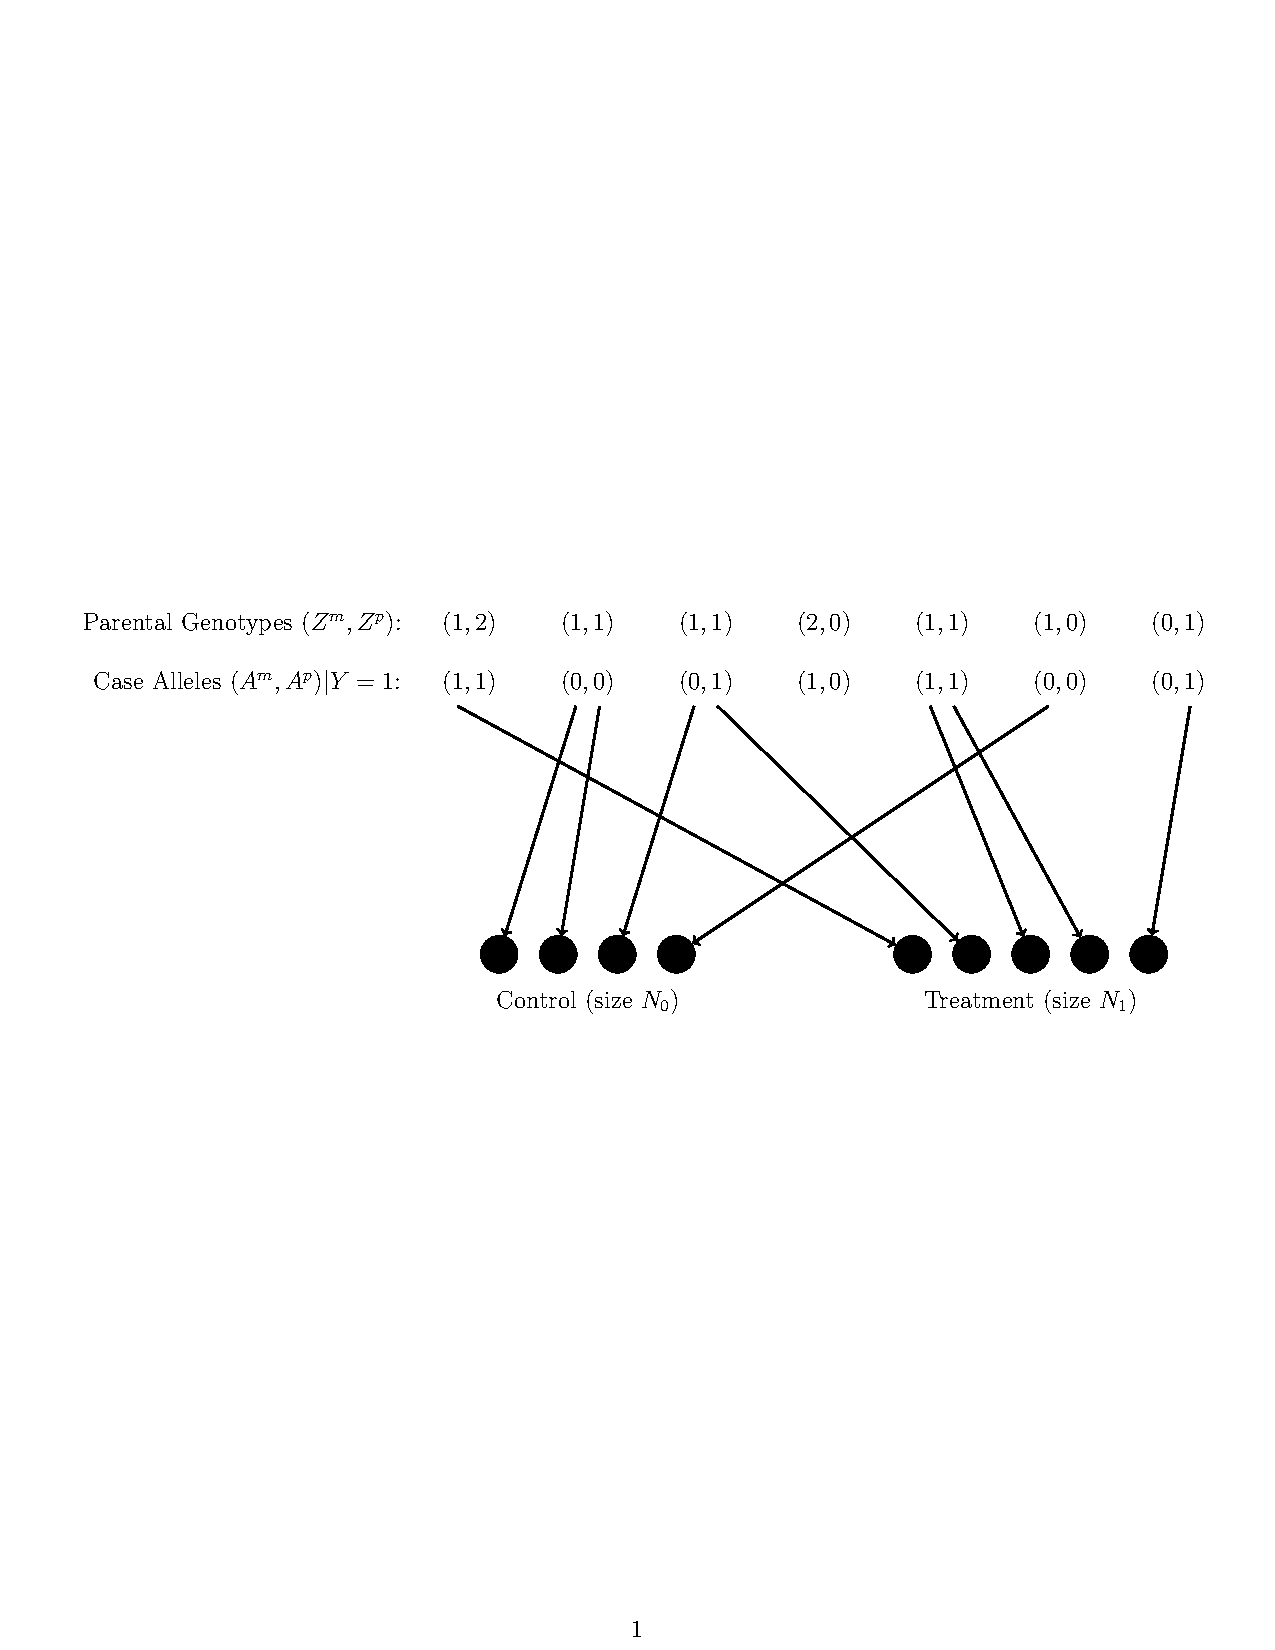
\includegraphics[clip, trim=1.2cm 10.8cm 0cm 9cm, width = 1\textwidth]{./figures/figure2.pdf} % trim by left botm right top
\caption{\textbf{Schematic of the TDT assignment procedure.} If a heterozygous parent transmits an allele 0 to the affected child, an event (denoted by a solid dot) is recorded in the control. Alternatively, if transmitting an allele 1, an event is recorded in the treatment.}
\label{fig:tdt_procedure}
\end{figure}

We show that the TDT is a test of causality via the following theorem, which relies on our causal inference framework for the TMT.  We then show below that a component of the TDT statistic is an unbiased estimator of the causal effect analogous to $d_{\tmt}$. 
%\begin{mdframed}[style=mypre]
\begin{thm} \label{thm:tdt_ace}
The null hypothesis of TDT is true if and only if $\ace \big(G\to Y\big) = 0$. 
\end{thm}
%\end{mdframed} 

\begin{proof} We first construct a parameter analogous to the TMT parameter $\delta_{\tmt}$ under the TDT setting by defining a TDT parameter $\delta_{\tdt}$, which involves a factor that accounts for the affected-only sampling. Suppose the affected children are sampled from a population where the disease prevalence given parental heterozygote is 
\begin{align*}
\eta &= \pp(Y=1|Z=1,N),\,\,\, 0< \eta <1.
\end{align*} Note that $\eta$ is not needed for the test but just for bridging the TDT and the TMT. 

\begin{defin}[TDT parameter]\label{def:tdt_param}
Define the TDT parameter $\delta_{\tdt}$ such that  
\begin{align*}
\delta_{\text{TDT}} &= \eta \E[\indicator(A^m=1)-\indicator(A^m=0)|Y=1,Z^m=1,N] ~ \\
& \qquad + \eta \E[\indicator(A^p=1)-\indicator(A^p=0)|Y=1,Z^p=1,N].
\end{align*}
\end{defin} 

\noindent A relevant difference between the TDT and the TMT for dichotomous traits is that the original TDT only samples trios with the child's trait value $Y_j=1$, whereas the causal framework for the TMT is based on trios with the child's trait value $Y_j=1$ and $Y_j=0$ randomly sampled from the underlying population. To fit the TDT under the causal framework for the TMT, we derive causal properties of the TDT with respect to the underlying population with both $Y_j=1$ and $Y_j=0$. We explain the connection between $\delta_{\tdt}$ and $\delta_{\tmt}$ as the following.

\begin{lem} \label{lem:delta_tdt} 
When the trait only takes two values, such that $Y \in \{0,1\}$, then $\delta_{\text{TDT}}=\delta_{\text{TMT}}$. 
\end{lem} 

\noindent We prove \Cref{lem:delta_tdt} in \Cref{app:delta_tdt}. It implies the equivalence between $\delta_{\tdt}$ and $\delta_{\tmt}$ for binary traits. It enables developing an estimand for $\delta_{\tdt}$ in a similar format as the TMT estimand $d_{\tmt}$. To this end, we consider the following unbiased TDT estimand. 

\begin{defin}[TDT estimand] \label{def:dtdt}
The TDT estimand is defined as:
\begin{align}
& d_{\tdt} = \frac{2}{N}(N_1-N_0) = \frac{2}{N}\sum_{j\in \cJ}(W_{1j}-W_{0j})Y_j,
\end{align}
where $Y_j = 1$ for all $j \in \cJ$.
\end{defin}
\noindent Note that $d_{\tdt} = d_{\tmt}$ when $Y_j = 1$ for all $j \in \cJ$.

\begin{lem} \label{lem:tdt_ace} 
Under the trait model in \Cref{eq:app_gtm}, $d_{\tdt}$ is unbiased for $\delta_{\tdt}$ in that 
\begin{align*}
\E[d_{\tdt}|N] &= \delta_{\tdt}.
\end{align*}
\end{lem}

\noindent We prove \Cref{lem:tdt_ace} in \Cref{app:tdt_ace}. 

To connect $d_{\tdt}$ to the original TDT test statistic, consider $d^{\ast}_{\tdt}=d_{\tdt}/2=(N_1-N_0)/N$, which is the difference between the proportion of alleles 1 ($N_1/N$) and the proportion of alleles 0 ($N_0/N$) transmitted from affected child's heterozygous parents. The theory of McNemar's statistic \citep{mcnemar1947} utilizes the following component 
\begin{align*}
\sigma^2_{d^{\ast}_{\tdt}} &= \frac{N_1/N+N_0/N}{N} = \frac{N_1+N_0}{N^2}
\end{align*} to derive a test statistic that equals $\chi^2$ with one degree of freedom as 
\begin{align*}
\chi_{\text{TDT}}^2 &= \frac{(d^{\ast}_{\tdt})^2}{\sigma^2_{d^{\ast}_{\tdt}}}=\frac{\big((N_1-N_0)/N\big)^2}{(N_1+N_0)/N^2}=\frac{(N_1-N_0)^2}{N_1+N_0}.
\end{align*} Therefore, the original TDT is equivalent to testing $H_0: \delta_{\tdt}=0$ vs. $H_1: \delta_{\tdt}\neq 0$. By \Cref{lem:delta_tdt}, $\delta_{\tdt}\neq 0$ if and only if $\delta_{\tmt}\neq 0$. By \Cref{thm:tmt_ace}, $\delta_{\tmt}\neq 0$ if and only if $\ace \big(G \to Y\big)\neq 0$. Thus $\delta_{\tdt}\neq 0$ if and only if $\ace(G\to Y)\neq 0$, which completes the proof for \Cref{thm:tdt_ace}.  \end{proof}

\subsection{Detecting causal linkage via the TMT and TDT} \label{sec:causal_linkage}

%\begin{asm}\label{asm:law_segregation}
%Under the trait model in \Cref{eq:app_gtm},
%
%\begin{align*}
%\pp(A=a|Z=1) &= \pp(A=a|Z=1, \gamma), \quad a\in \{0,1\}.
%\end{align*} 
%\end{asm}

%\begin{equation} \label{eq:app_gtm}
%\begin{aligned}
%Y &= \alpha_0\indicator(A^m+A^p=0) + \alpha_1 \indicator(A^m+A^p=1) + \alpha_2 \indicator(A^m+A^p=2) + \gamma \\
%&= \alpha_0\indicator(G=0) + \alpha_1 \indicator(G=1) + \alpha_2 \indicator(G=2) + \gamma.
%\end{aligned}
%\end{equation}
%
%\begin{align}
%Y^m(0) &= \alpha_0\indicator(A^p=0) + \alpha_1\indicator(A^p=1) + \gamma, \\
%Y^m(1) &= \alpha_1\indicator(A^p=0) + \alpha_2\indicator(A^p=1) + \gamma, \\
%\end{align}

%{eq:potentialoutcomes}
%
%{asm:law_segregation}

Here, we consider the case where a genetic marker is linked to a causal variant, due to population-level linkage disequilibrium, within-trio meiotic genetic linkage, or both. Suppose that marker $c$ is causal while non-causal marker $d$ is linked to $c$. Since $c$ is causal the trait model from \Cref{eq:app_gtm} is $Y = \alpha_{c0} \indicator(G_c=0) + \alpha_{c1} \indicator(G_c=1) + \alpha_{c2} \indicator(G_c=2) + \gamma_c$, where the assumptions required for the TMT and TDT hold. A key assumption is \Cref{asm:law_segregation}, where it is assumed that $\pp(A_c = a | Z_c = 1) = \pp(A_c = a | Z_c = 1, \gamma_c)$ for $a \in \{0,1\}$. For a causal locus, this is a plausible assumption as explained when that assumption was introduced. However, for locus $d$ where $G_c$ and $G_d$ may be dependent, the assumption when modeling $Y$ in terms of $G_d$ may be violated. 

We can write the trait model in terms of both genotypes $G_c$ and $G_d$ as
\begin{align*}
Y & = \alpha_{c0} \indicator(G_c=0) + \alpha_{c1} \indicator(G_c=1) + \alpha_{c2} \indicator(G_c=2) + \gamma_c \\
  & = \alpha_{d0} \indicator(G_d=0) + \alpha_{d1} \indicator(G_d=1) + \alpha_{d2} \indicator(G_d=2) + \gamma_d,
\end{align*} where
\begin{equation*}
\gamma_d = \alpha_{c0} \indicator(G_c=0) + \alpha_{c1} \indicator(G_c=1) + \alpha_{c2} \indicator(G_c=2) + \gamma_c.
\end{equation*}
Since $c$ is causal it follows that $\alpha_{c1} - \alpha_{c0} \not= 0$ or $\alpha_{c2} - \alpha_{c1} \not= 0$. Since $d$ is not causal, it should be the case that $\alpha_{d0} = \alpha_{d1} = \alpha_{d2}$ = 0. In order to investigate the behavior of the TMT and TDT applied to marker $d$, we need to determine if $\pp(A_d = a | Z_d = 1) = \pp(A_d = a | Z_d = 1, \gamma_d)$ for $a \in \{0,1\}$. (Note that when $Z_d \not= 1$, then the transmission from this parent is not included in the TMT or TDT.) This may not be the case since $G_c$ and $G_d$ are dependent, so $A_c$ and $A_d$ may be dependent. Further, $\gamma_d$ is a function of $A_c$ (and $G_c$). 

For a given parent, the dependence between $A_d$ and $\gamma_d$ is driven by $A_c$, so we will determine if $\pp(A_d = a | Z_d = 1) = \pp(A_d = a | Z_d = 1, A_c)$ for $a \in \{0,1\}$ by specifically calculating $\pp(A_d = a, A_c=b | Z_d = 1)$ for $a, b \in \{0,1\}$. When $Z_c = 0$, then $A_c=0$ with probability 1 and when $Z_c = 2$, then $A_c=1$ with probability 1. Thus, 
\begin{align*}\pp(A_d = a, A_c=0 | Z_d = 1, Z_c=0) & = \pp(A_d = a | Z_d = 1, Z_c=0) \\
 & = \pp(A_d = a | Z_d = 1) \\
 & = \pp(A_d = a | Z_d = 1) \pp(A_c = 0 | Z_c = 0) 
\end{align*}
for $a \in \{0, 1\}$. The analogous result holds when $Z_c = 2$. One can conclude from this that when $Z_c = 0$ or $Z_c = 2$, then the required assumption to validly test marker $d$ for causality holds for this parent-child combination. 

This leaves the case of $Z_c = 1$. A given parent has two haplotypes from among the four possible haplotypes, $\{(0,0), (0,1), (1,0), (1,1)\}$. Let $H_{cd}$ be the set of two haplotypes of the parent. Given that $Z_c = 1, Z_d = 1$, the possible haplotypes are $H_{cd} = \{(0,0), (1,1)\}$ or $H_{cd} = \{(0,1), (1,0)\}$. Let 
\begin{align*}\eta_{cd} & = \pp(H_{cd} = \{(0,0), (1,1)\} | Z_c = 1, Z_d = 1), \\
1- \eta_{cd} & = \pp(H_{cd} = \{(0,1), (1,0)\} | Z_c = 1, Z_d = 1).
\end{align*}
Also, let $\theta_{cd}$ be the meiotic recombination rate between loci $c$ and $d$. It then follows that

\begin{equation} \label{eq:jointprobs}
\begin{aligned}
\pp(A_d = 1, A_c = 1 | Z_d = 1, Z_c = 1) & = \frac{1}{2} \eta_{cd} (1 - \theta_{cd}) + \frac{1}{2} (1-\eta_{cd}) \theta_{cd} \\
 & =  \pp(A_d = 0, A_c = 0 | Z_d = 1, Z_c = 1) \\
 &  \\
\pp(A_d = 0, A_c = 1 | Z_d = 1, Z_c = 1) & = \frac{1}{2} (1-\eta_{cd}) (1 - \theta_{cd}) + \frac{1}{2} \eta_{cd} \theta_{cd} \\
 & =  \pp(A_d = 1, A_c = 0 | Z_d = 1, Z_c = 1) 
  \end{aligned}
\end{equation}

Based on \Cref{eq:jointprobs}, it is trivial to show that $\pp(A_c = a | Z_c = 1, Z_d = 1) = 1/2$ for $a \in \{0, 1\}$ regardless of the values of $\eta_{cd}$ and $\theta_{cb}$. We have also shown earlier that $\pp(A = a | Z = 1) = 1/2$ for $a \in \{0, 1\}$ at any locus. It is therefore the case that 
\begin{equation*}
\pp(A_d = a, A_c = b | Z_d = 1, Z_c = 1) = \pp(A_d = a | Z_d = 1) \pp(A_c = b | Z_c = 1)
\end{equation*}
for $a, b \in \{0, 1\}$ whenever the quantities in \Cref{eq:jointprobs} equal $1/4$, which holds if and only if either $\eta_{cd} = 1/2$ or $\theta_{ab} = 1/2$. Note that the it does not need to be the case that $\eta_{cd} = \theta_{ab} = 1/2$; only one of the parameters needs to equal $1/2$.

When markers $c$ and $d$ are in linkage equilibrium, it will be the case that $\eta_{cd} = 1/2$, and when markers $c$ and $d$ are genetically unlinked (in the meiotic sense), it will be the case that $\theta_{ab} = 1/2$. When \textit{both} of these do not hold, then the randomization at marker $d$ is probabilistically dependent with the randomization at $c$ and we say that these markers have \textit{randomization linkage}. This implies that the null hypothesis of marker $d$ is not true when marker $c$ is causal. In this case we say that $d$ is in \textit{causal linkage} with $Y$, formalized in the following definition.

\begin{defin}[Causal linkage of alleles]\label{def:causal_link}
Suppose marker $c$ is directly causal for $Y$, where $A_c$ satisfies \Cref{def:direct_causality} in that $\ace(A_c\to Y)\neq 0$. Locus $d$ is in ``causal linkage'' with the trait $Y$ if it has both linkage disequilibrium and meiotic genetic linkage with marker $c$.  We denote causal linkage by $A_d \hookrightarrow Y$.
\end{defin} 

\noindent If an allele $A$ is itself directly causal for $Y$, then this allele $A$ is trivially in causal linkage with $Y$ since it is in complete linkage with itself. Thus, $A \to Y \Rightarrow A \hookrightarrow Y$.

\begin{defin}[Causal linkage of genotypes] \label{def:causal_link_geno}
For the child's genotype $G_d=A^m_d+A^p_d$, we say $(A^m_d,A^p_d) \hookrightarrow Y$ if either $A^m_d \hookrightarrow Y$ or $A^p_d \hookrightarrow Y$.
\end{defin}

\begin{lem}\label{lem:causal_link}
For the TMT, $\delta_{\tmt}\neq 0$ at marker $d$ only if $(A^m_d,A^p_d) \hookrightarrow Y$. For the TDT, $\delta_{\tdt}\neq 0$ at marker $d$ only if $(A^m_d,A^p_d) \hookrightarrow Y$.
\end{lem}

\noindent We prove \Cref{lem:causal_link} in \Cref{app:causal_link}. It enables the identification of causal linkage by testing non-zero $\delta_{\tmt}$ via the TMT and non-zero $\delta_{\tdt}$ via the TDT. The test statistics $d_{\tmt}$ and $d_{\tdt}$ can be utilized to characterize the signal of causal linkage by genome-wide TMT or TDT profiles shown in \Cref{sec:tmt_tdt_profile}. Under simulations reflecting levels of linkage disequilibrium observed in humans, it does not appear that causal linkage is an impediment to identifying causal loci. Under the theoretical calculations done above, it can be seen that the power is greater at $c$ relative to $d$, and this is what we also observe empirically. It has been suggested that under Haldane's model of recombination one can break the genome into independent blocks, which would allow us to test for causality at the resolution of these blocks \citep{bates2020}. However, empirical evidence suggests that Haldane's model of recombination does not hold in the human genome \citep{myers2005, coop2008, kivikoski2023}. % It seems that the complex probabilistic dependence among genetic markers is a fundamental property of genetics that may not be avoidable under current study designs and technologies.

\section{Numerical Results}

\subsection{Evaluation of the TMT as a test of causality} \label{sec:tmt_empirical}

\paragraph{Simulating trio genotypes.}

We simulated trio data to evaluate the accuracy and power of the TMT. We sampled the parental genotypes $\boldsymbol{Z}$ from a structured population based on a standard admixture model \citep{PSD2000, falush2003, ochoa2021} of four intermediate sub-populations (\Cref{app:sim_trio_geno}). We followed an established pipeline \citep{ochoa2021} to simulate intermediate subpopulations while keeping the overall $F_{\text{ST}} = 0.2$. (See \Cref{fig:pop_structure} for a visualization of pairwise relatedness in the structured population through co-ancestry coefficients.) We then simulated the alleles $(A_{ij}^m,A_{ij}^p)$ by randomly drawing one transmitted allele from corresponding parental genotypes $(Z_{ij}^m,Z_{ij}^p)$, yielding the child's genotype $G_{ij}=A_{ij}^m+A_{ij}^p$.

\paragraph{Simulating child's phenotypes.}

To simulate the child's trait $\boldsymbol{Y}=\{Y_j\}$ (see the schematic in \Cref{fig:y_simulate}), we implemented a trait model with genetic effects from multiple loci in \Cref{eq:ptm_with_e}. Let $\cC$ be the index set of causal loci. The traits are generated according to:
\begin{align} 
Y_j &= \intercept + \sum_{i\in \cC}\Big( \alpha_0\indicator(G_{ij}=0) + \alpha_1\indicator(G_{ij}=1) + \alpha_2\indicator(G_{ij}=2) \Big)+\beta E_j+\epsilon_j,
\label{eq:ptm_with_e}
\end{align} 
where $(\iota,\beta)$ are scalar values, $(\alpha_0,\alpha_1,\alpha_2)$ are genetic effects per locus (made equal for all causal loci), and $\epsilon_j$ is the independent non-genetic random variation drawn from $\mathcal{N}(0,\sigma_e^2)$. The random variable $E_j$ is the non-genetic variation constructed to also be a function of the population structure. Therefore, $E_j$ is a confounder between the genotypes and the trait, and the parameter $\beta$ allows us to modulate the effect size of this confounder. Simulation details about $E_j$ are summarized in \Cref{app:sim_quant_trait}, where we also show that \Cref{eq:ptm_with_e} satisfies the trait model in \Cref{eq:app_gtm}. Note that the ratio $(\alpha_2-\alpha_1)/(\alpha_1-\alpha_0)$ can be any numerical value under the trait model in \Cref{eq:app_gtm}. When $(\alpha_2-\alpha_1)/(\alpha_1-\alpha_0)=1$, it is equivalent to an additive polygenic trait model. We display the result for $(\alpha_2-\alpha_1)/(\alpha_1-\alpha_0)=1$ in \Cref{fig:tmt_ace} and other $(\alpha_2-\alpha_1)/(\alpha_1-\alpha_0)$ values in \Cref{fig:tmt_various_parameters}. We set $\intercept=100$ and note that any value of $\intercept$ should work because $\intercept$ would be subtracted from $Y_j$ after centering by $\hat{\mu}_c$ in \Cref{eq:dtmt}.

\begin{figure}
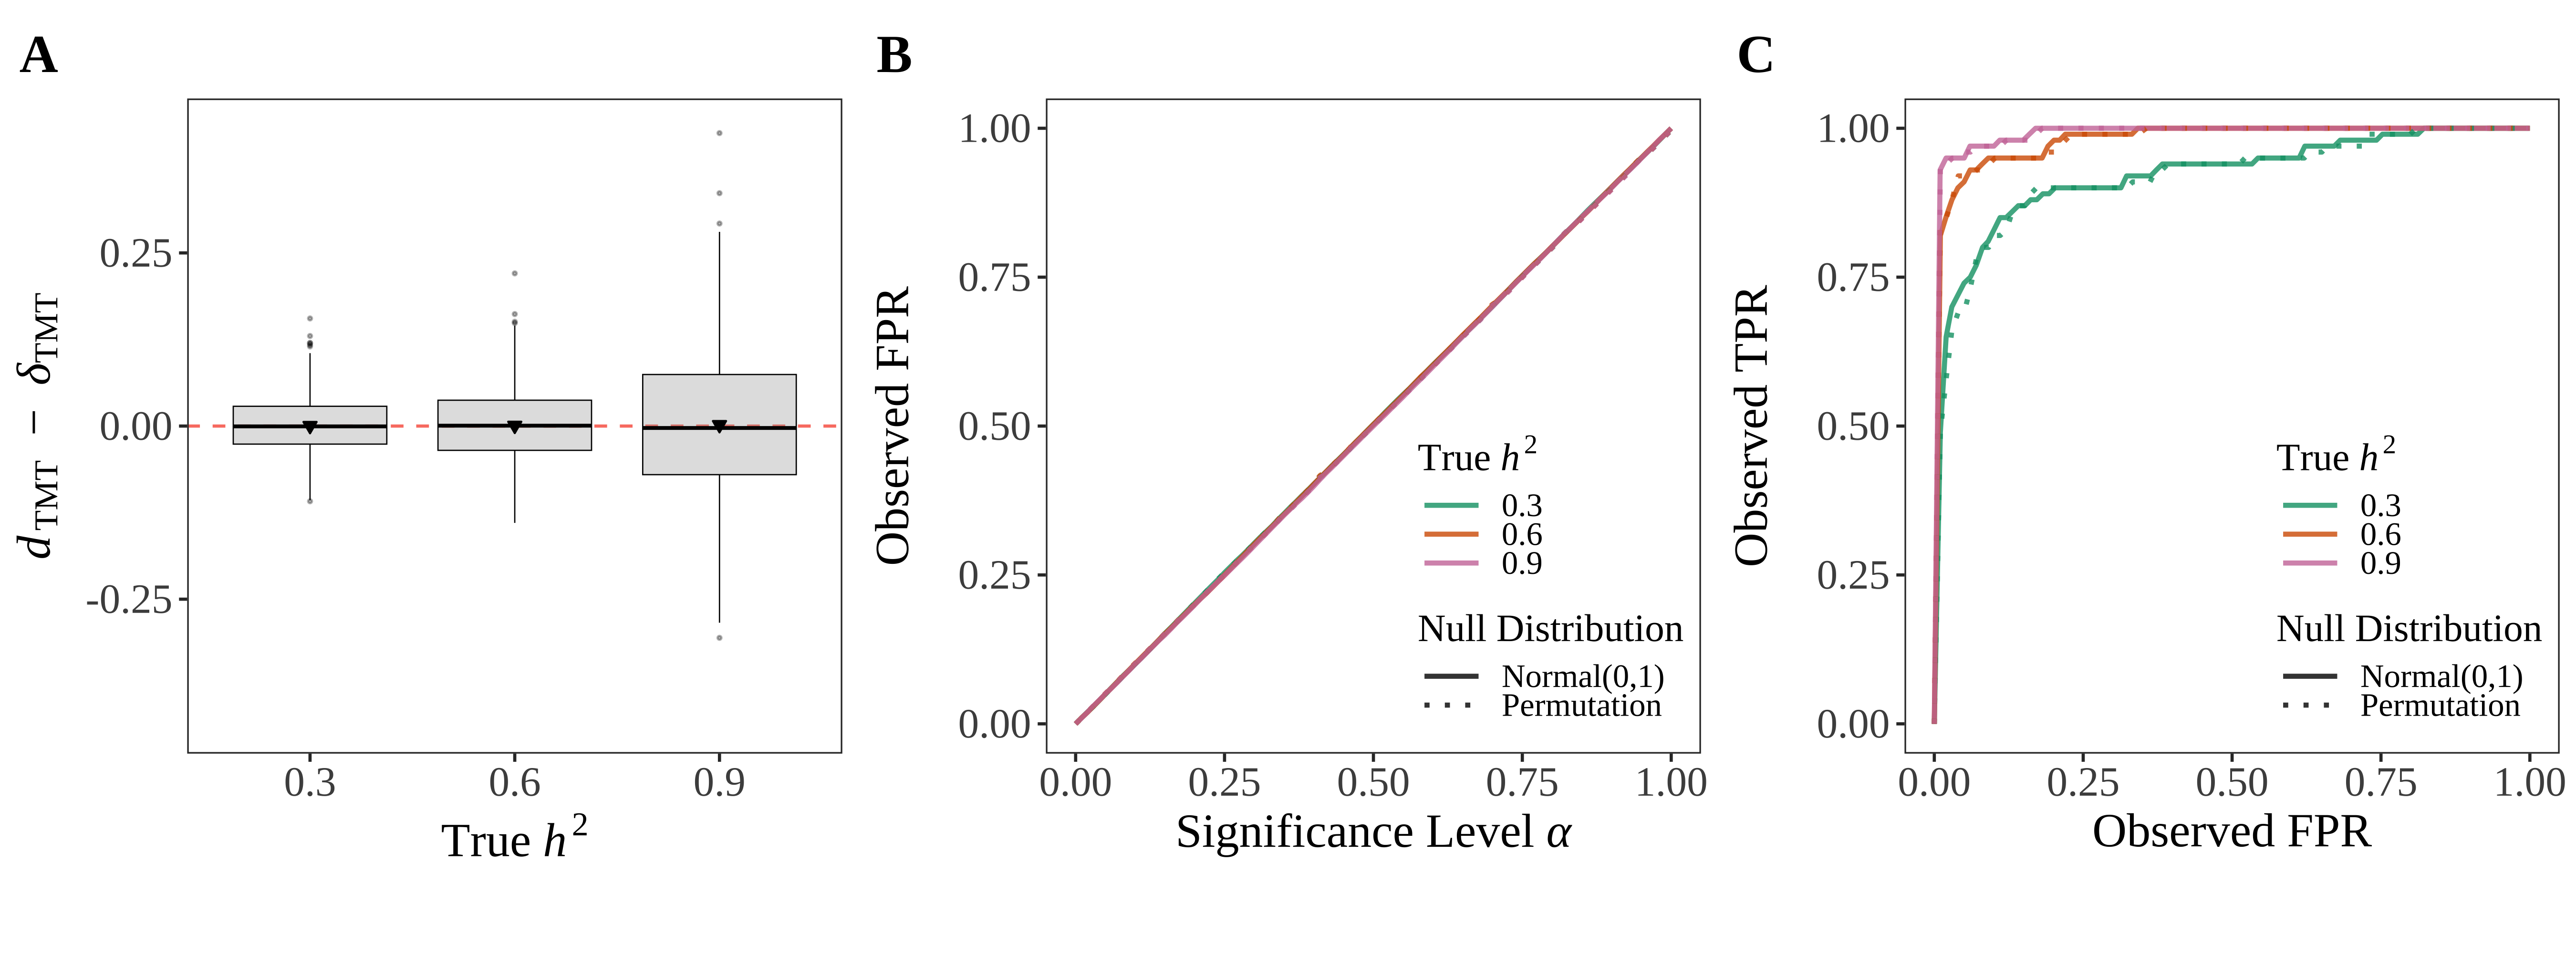
\includegraphics[clip, trim=0cm 2cm 0cm 0cm, width = 1\textwidth]{./figures/figure3.png} % trim by left botm right top
\caption{\textbf{The TMT is a valid test of causality. (A)} $d_{\tmt}$ is an unbiased estimator of $\delta_{\tmt}$. We followed \Cref{app:sim_trio_geno} to generate 5,000 trios from a structured population ($F_{ST}=0.2$) with 100,000 SNPs per individual and we randomly chose 100 loci to be causal. We simulated the child traits at the heritability levels ($h^2\in \{0.3,0.6,0.9\}$) based on \Cref{app:sim_quant_trait}. Shown are 1000 randomly chose instances of $d_{\tmt}-\delta_{\tmt}$ for each heritability level. \textbf{(B)} The TMT controls the FPR at the desired significance level per experiment. \textbf{(C)} The ROC curve from a randomly chosen simulated data set. Both the Normal$(0,1)$ (solid lines) and permutation (dotted lines) null distributions are shown.}
\label{fig:tmt_ace}
\end{figure}

%We then randomly selected one causal locus to calculate $d_{\tmt}$. To enter the second round of simulation, we kept parental genotypes and randomly drew transmitted alleles to generate a new matrix of the child's genotypes. Then we followed \Cref{app:sim_quant_trait} to simulate the child's trait. At the same causal locus for the previous round, we calculated $d_{\tmt}$ and $\delta_{\tmt}$. 

%For (B) and (C), we implemented the TMT to calculate $p$-values across all 100,000 SNPs in a single round of simulation. Given a significance level $\alpha$, we derived the observed FPR and TPR to be presented in (B) and (C). 

\paragraph{Point estimation of ACE.}

We numerically confirmed the accuracy of $d_{\tmt}$ as an unbiased estimate of the TMT parameter $\delta_{\tmt}$ to detect non-zero ACE in \Cref{def:ace} across various values of $h^2$ (\Cref{fig:tmt_ace}A). The unbiasedness of $d_{\tmt}$ is immune to the confounding effects from the population structure and non-genetic factors that are associated with the population structure. 

\paragraph{Causal FPR and the ROC curve.}

We performed the TMT at each locus and calculated $p$-values for both causal and non-causal SNPs by utilizing both the Normal$(0,1)$ theoretical null distribution and the permutation null. We then computed the false positive rate (FPR) and the true positive rate (TPR) for causal loci at various significance thresholds between 0 and 1. The TMT strictly controls the FPR at the desired significance level across all levels of $h^2$ (\Cref{fig:tmt_ace}B). The receiver operating characteristic (ROC) curve demonstrates the TMT having statistical power for detecting directly causal effects for all levels of $h^2$, especially when $h^2$ is high (\Cref{fig:tmt_ace}C). Besides the standard Normal$(0,1)$ null distribution, we also used a permutation null distribution to calculate a $p$-value by following \Cref{app:permutation_test}. The two null distributions show similar performance (\Cref{fig:tmt_ace}B and C). 

\paragraph{Validation of theoretical null distribution.}

We started from a small sample of 100 trios and permuted $\boldsymbol{Y}$ to generate the null distributions of the test statistic $\tau_{\tmt}$ from \Cref{eq:tau_tmt}. Our results validated that $\tau_{\tmt}$ follows the Normal$(0,1)$ distribution (\Cref{fig:tmt_t_null}). Considering that population-based trio studies usually contain at least a few hundred families, the Central Limit Theorem underlying the Normal$(0,1)$ null distribution for $\tau_{\tmt}$ seems to be applicable.


\subsection{Evaluation of the TDT as a test of causality} \label{sec:tdt_empirical}

\begin{figure}
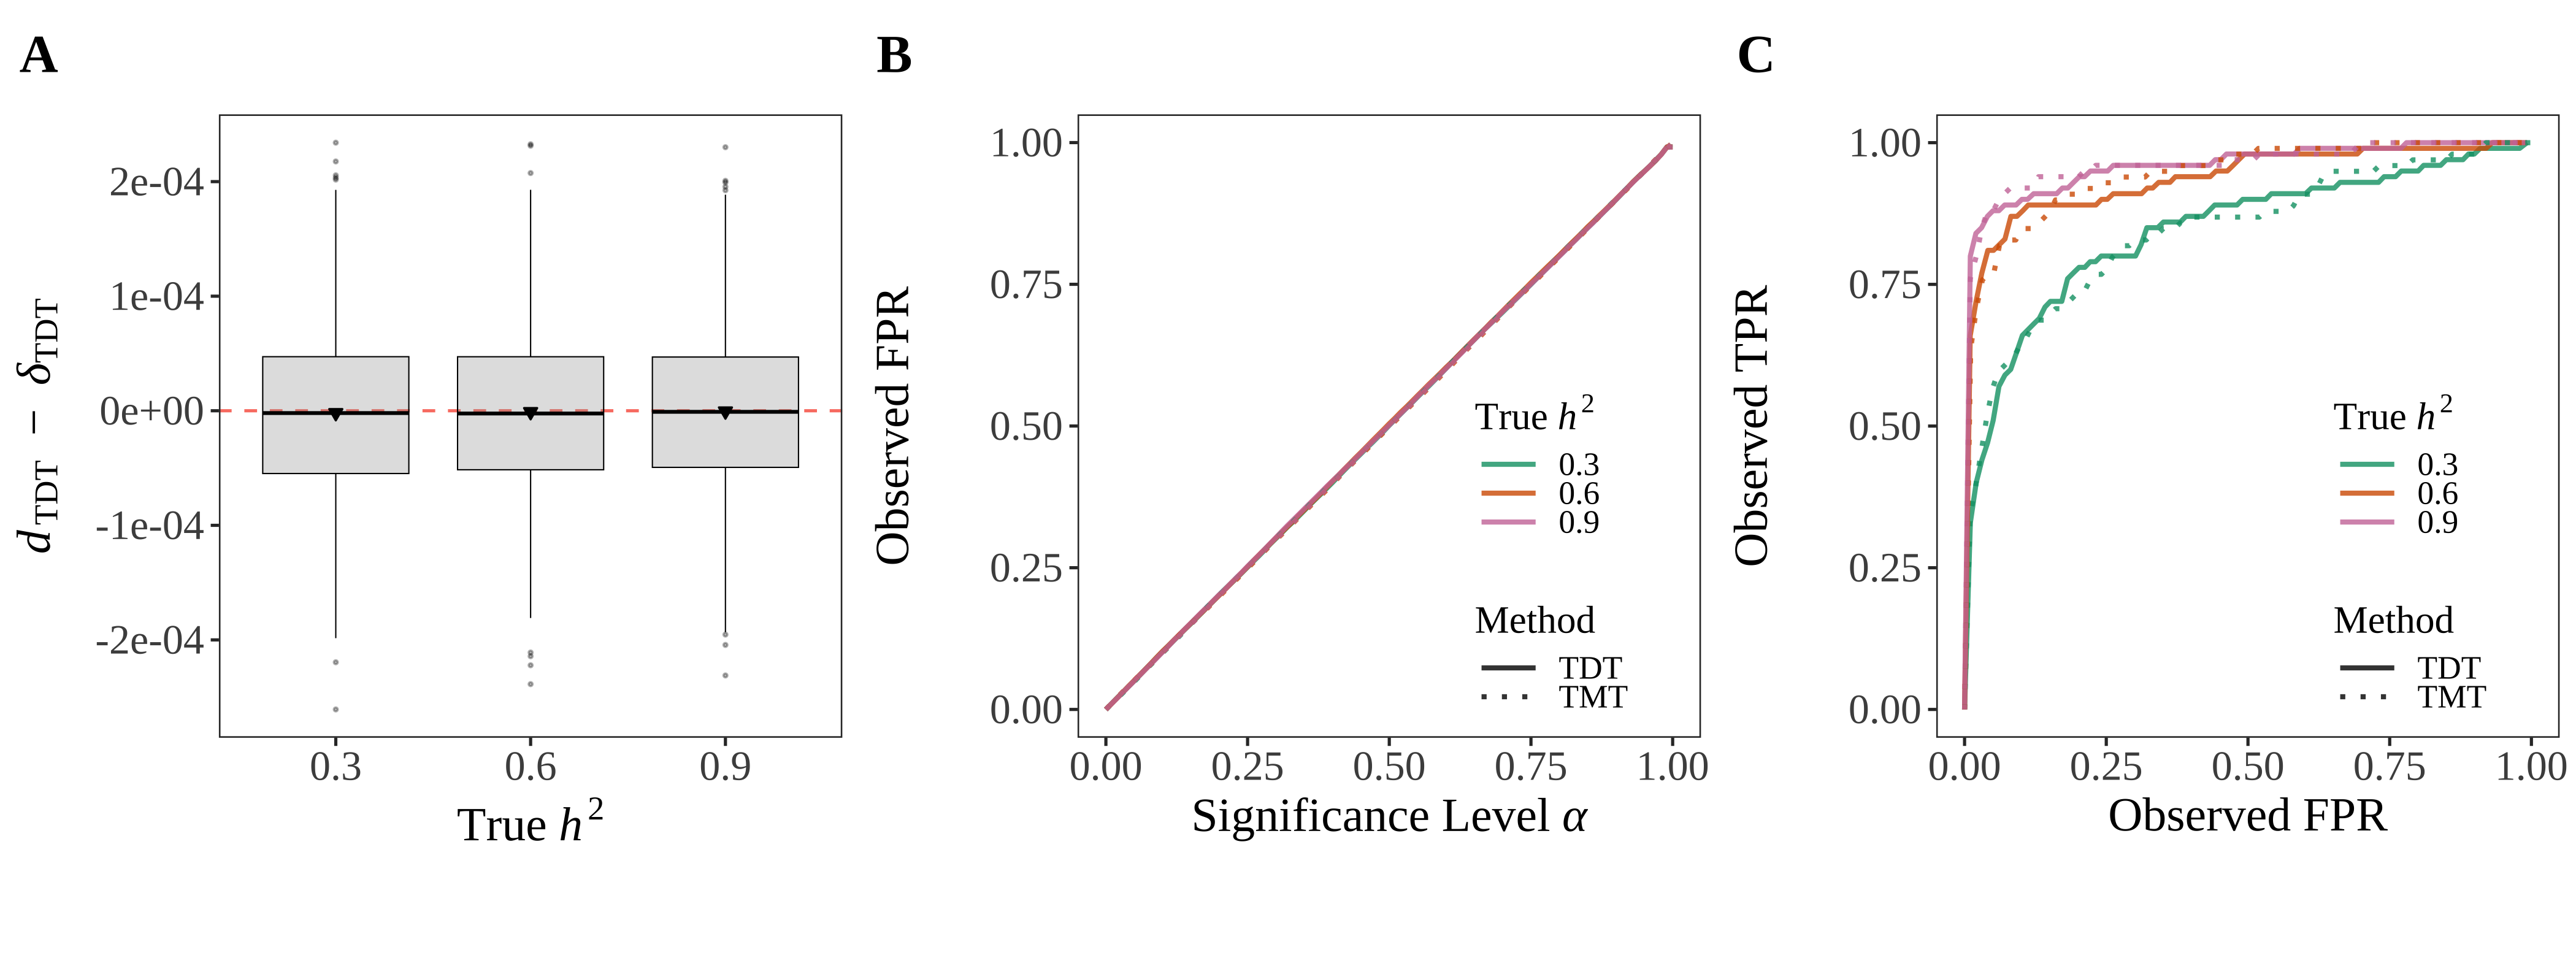
\includegraphics[clip, trim=0cm 0cm 0cm 0cm, width = 1\textwidth]{./figures/figure4.png} % trim by left botm right top
\caption{\textbf{The TDT is a valid test of causality. (A)} $d_{\tdt}$ is an unbiased estimator of $\delta_{\tdt}$. We simulated 5000 affected-only trios based on the description in the text. We then calculated $d_{\tdt}$ and performed the TDT. Each box plot shows 1000 randomly chosen instances of $d_{\tdt}-\delta_{\tdt}$ at each heritability level. \textbf{(B)} The TDT and TMT control FPR at the desired significance level. We additionally applied the TMT to 5000 randomly chosen trios composed of an equal number of normal and affected children. We calculated the FPR for the TDT and TMT across a range of thresholds as shown. \textbf{(C)} The ROC curve for a randomly chosen data set for both the TDT and TMT.}
\label{fig:tdt_ace}
\end{figure}

%Each box contains 1,000 simulations. In the first round of simulation, we followed \Cref{app:sim_trio_geno} to generate 10,000 trios from a structured population ($F_{ST}=0.2$) with 100,000 SNPs per individual and randomly chose 100 directly causal loci out of the child's genotypes. For the child's trait, we simulated a continuous latent variable at the desired heritability levels ($h^2\in \{0.3,0.6,0.9\}$) based on \Cref{eq:ptm_with_e_tdt}. We used the latent variable to generate dichotomous trait based on \Cref{app:sim_binary_trait} given a disease prevalence 0.5, resulting in 5,000 affected children and 5,000 normal ones. We then randomly selected one causal locus to calculate $d_{\tdt}$. To enter the second round of simulation, we kept parental genotypes and randomly drew transmitted alleles to generate a new matrix of the child's genotypes. Then we repeat the above pipeline to simulate the child's binary trait. At the same causal locus for the previous round, we calculated $d_{\tdt}$ and $\delta_{\tdt}$. We repeated this procedure for 1,000 times and we presented all $d_{\tdt}-\delta_{\tdt}$ as (A).

As with the TMT evaluation, we followed the trio genotypes simulation pipeline in \Cref{app:sim_trio_geno} to simulate 10,000 trios with 100,000 SNPs per individual. Among the child genotypes $\boldsymbol{G}=\{G_{ij}\}$, we randomly chose 100 directly causal loci. To simulate a dichotomous trait, we first generated a continuous latent variable $\boldsymbol{L}=\{L_j\}$ by 
\begin{align} \label{eq:ptm_with_e_tdt}
L_j &= \intercept + \sum_{i\in \cC}\Big( \alpha_0\indicator(G_{ij}=0) + \alpha_1\indicator(G_{ij}=1) + \alpha_2\indicator(G_{ij}=2) \Big)+\beta E_j+\epsilon_j,
\end{align} where the parameter configuration is the same as \Cref{eq:ptm_with_e} used for the TMT evaluation. We then used the probit model (see \Cref{app:sim_binary_trait}) to convert $L_j$ into a dichotomous trait $Y_j$ according to a chosen disease prevalence. Children with $Y_j=0$ are labeled \textit{normal} and those with $Y_j=1$ are labeled \textit{affected}.

We applied the TDT on a per locus basis for trios with affected children and we also applied the TMT to a random subset of trios to match the sample size with the TDT. We computed the FPR and TPR across the range of significance levels. The TDT statistic $d_{\tdt}$ also demonstrates it is an unbiased estimate of the ACE for binary traits (\Cref{fig:tdt_ace}A). At all significance levels, the TDT controls the FPR at the desired level (as does the TMT) across all values of $h^2$ (\Cref{fig:tdt_ace}B). The ROC curves demonstrate similar and reliable statistical power of the TDT and the TMT for idenitifying causal loci (\Cref{fig:tdt_ace}C). 

\subsection{Genome-wide TMT profile and causal linkage} \label{sec:tmt_tdt_profile}

\begin{figure}
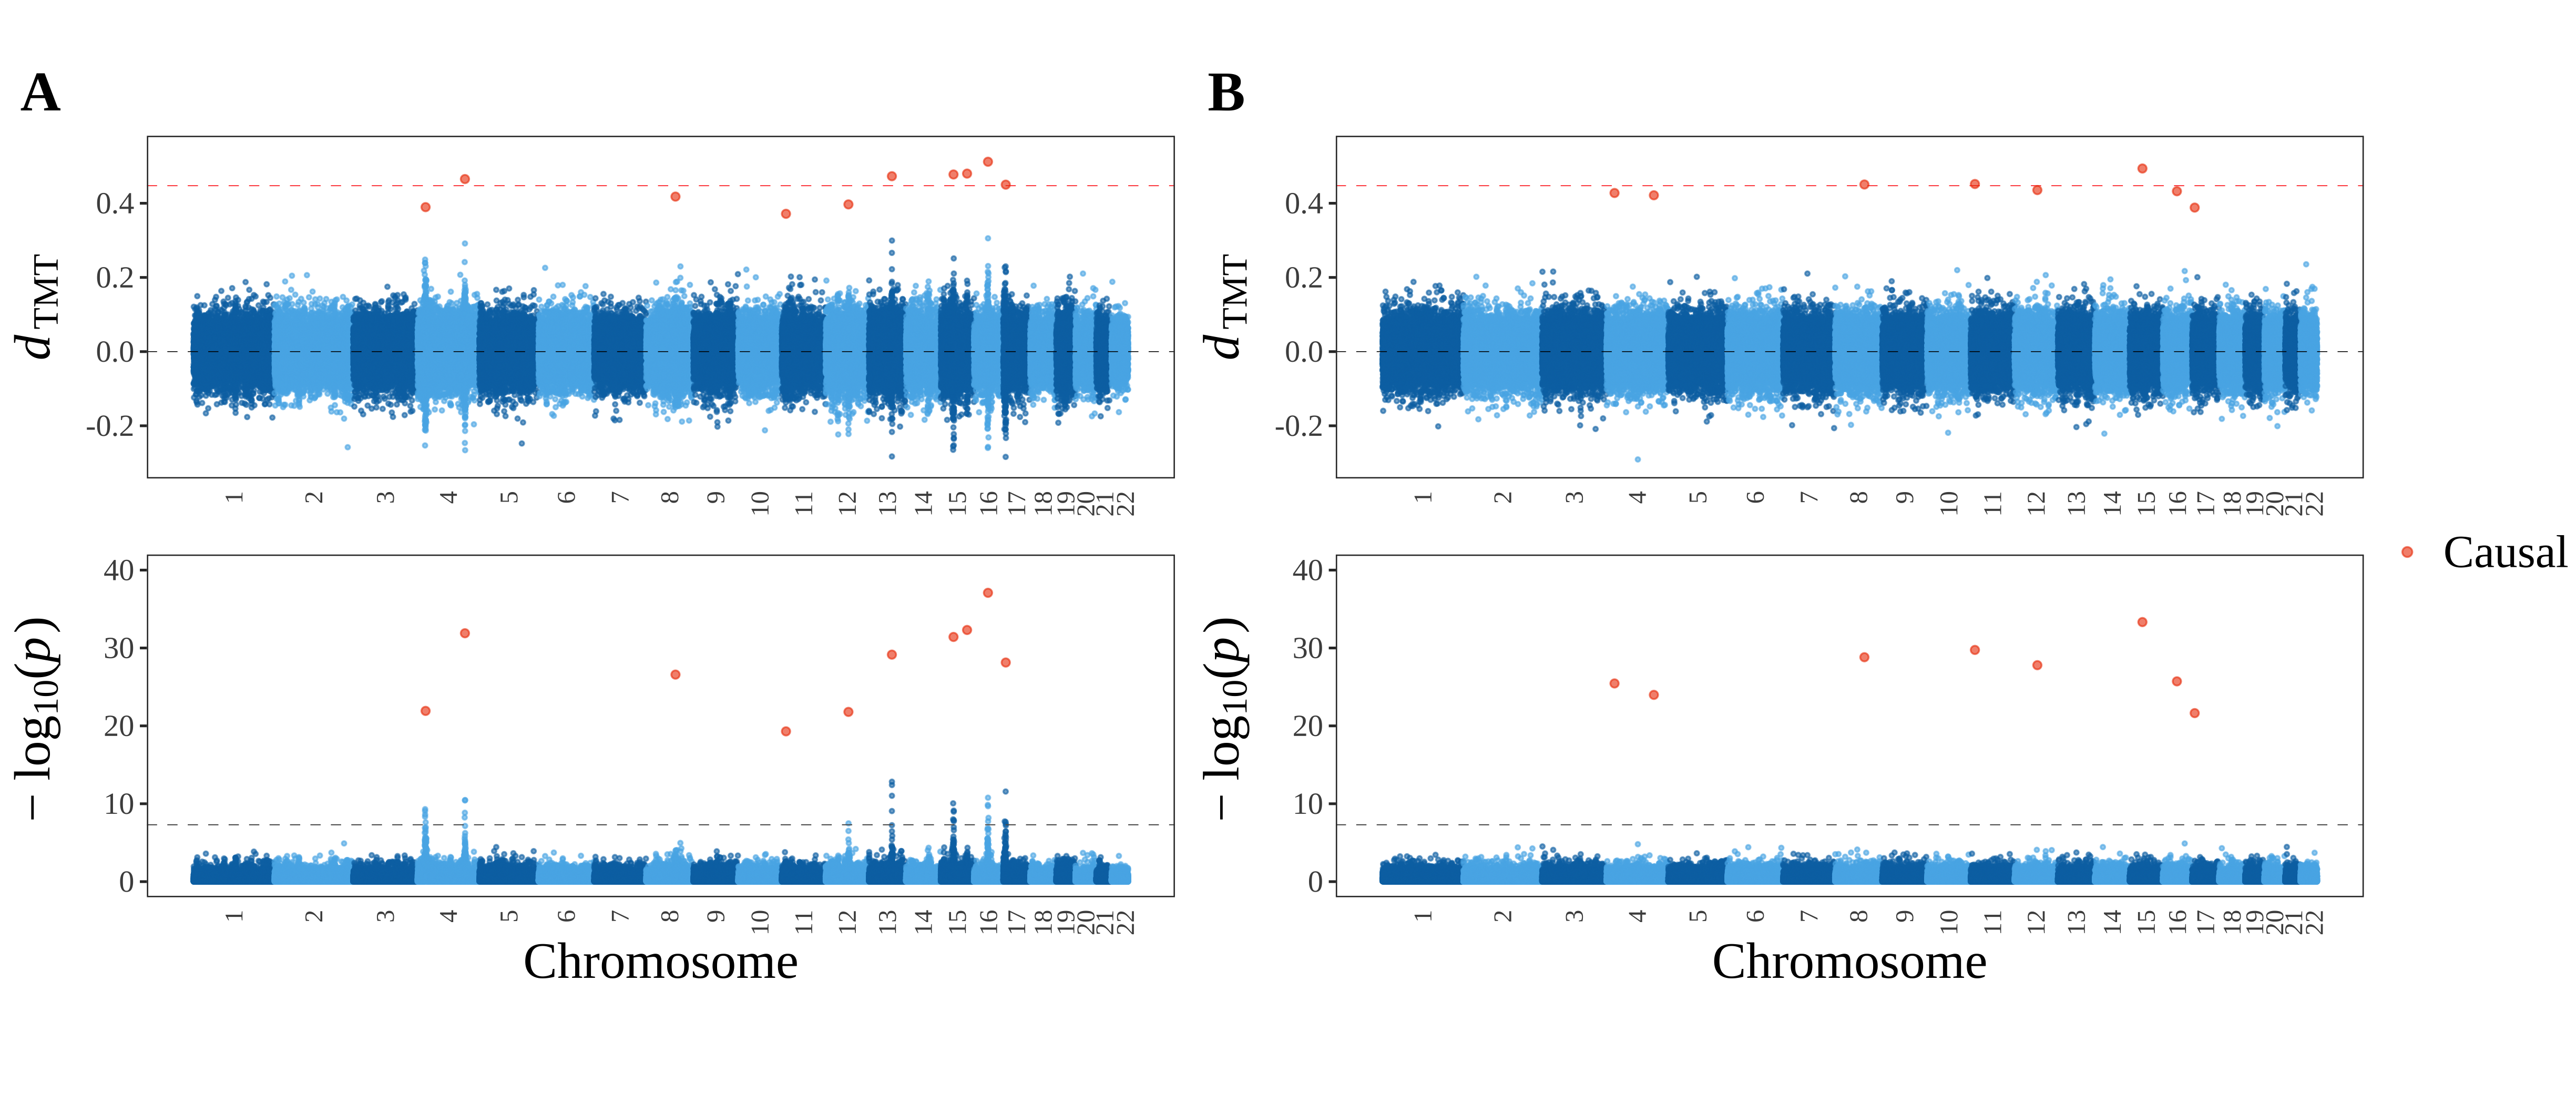
\includegraphics[clip, trim=0cm 2cm 0cm 0cm, width = 1\textwidth]{./figures/figure5.png} % trim by left botm right top
\caption{\textbf{The genome-wide TMT profile. (A)} Randomization linkage scenario. \textbf{(B)} Independent randomization scenario, where the genotypes from (A) were independently permuted to remove the randomization linkage. For both scenarios, the TMT profile is presented as $d_{\tmt}$ and $-\log_{10}$($p$) at 100,000 SNPs across 22 chromosomes simulated by \texttt{msprime}.  In the upper panel, the red dashed line is the true ACE at the causal loci and the black dashed line is for zero ACE at the non-causal loci. In the bottom panel, the gray dashed line is at $p$-value = $5\times 10^{-8}$, which is commonly used as a $p$-value threshold in GWAS.}
\label{fig:tmt_profile}
\end{figure} 

To empirically validate the TMT in the presence of causal linkage, we used the software \texttt{msprime} \citep{baumdicker2022} to simulate trio genotypes with linkage between SNPs. We generated a sample of 5,000 trios with 100,000 SNPs across 22 chromosomes per individual based on the American Admixture model \citep{browning2018} (simulation details in \Cref{app:simulate_genetic_linkage}). The level of linkage-disequilibrium (LD) in our simulated genotypes (\Cref{fig:ld}) matches previous findings observed in the human genome \citep{reich2001, dawson2002}. 

We first simulated a quantitative trait for the child phenotype to implement the TMT. Among the child genotypes $\boldsymbol{G}$, we randomly chose 10 causal SNPs denoted by set $\cC$. We generated the child phenotypes $\boldsymbol{Y}$ by the polygenic trait model $Y_j=\iota + \sum_{i\in \cC}bG_{ij} + \epsilon_j$ where we drew $\epsilon_j$ from Normal($0,\sigma^2_e$) and we set $\sigma^2_e=1$, $\iota=100$. The coefficient for causal SNPs, $b$, is determined such that $\V(\sum_{i\in \cC}bG_{ij})/\sigma^2_e=1$ (i.e., the heritability $h^2=0.5$). We displayed the TMT statistic $d_{\tmt}$ and corresponding $p$-values across all 100,000 SNPs as the genome-wide TMT profile (\Cref{fig:tmt_profile}A). To compare with linkage-equilibrium (LE), we permuted trio genotypes to remove genetic linkage, regenerated the child trait using the same parameters in the polygenic trait model above, and conducted the TMT on a per locus basis to derive $d_{\tmt}$ and $p$-values (\Cref{fig:tmt_profile}B). Under both LD and LE scenarios, the TMT shows accurate ACE estimation at the causal loci and yields a Uniform$(0,1)$ distribution of the $p$-values when the null hypothesis of non-causality is true. We also simulated a dichotomous trait and calculated the TDT statistic $d_{\tdt}$ and corresponding $p$-values to construct the genome-wide TDT profile under both LD and LE in \Cref{fig:tdt_profile}, where equivalent results were observed.


\subsection{TMT versus standard approaches in the presence of confounding}

Regression approaches, such as the ordinary least square (OLS) and linear mixed model (LMM), identify genotypes that are associated with phenotypes while making no claims of causality. The OLS approach does not account for population structure, whereas the LMM approach does. In order to guarantee that association tests from these two approaches yield correct p-value and false positive rate calculations, both approaches make a nontrivial assumption of exogeneity, which means that the non-genetic variation has zero covariance with the genetic variation. Thus, when confounding factors are present that conflate these two sources of variation, these methods may yield inaccurate results, even at the level of association. 

\begin{figure}
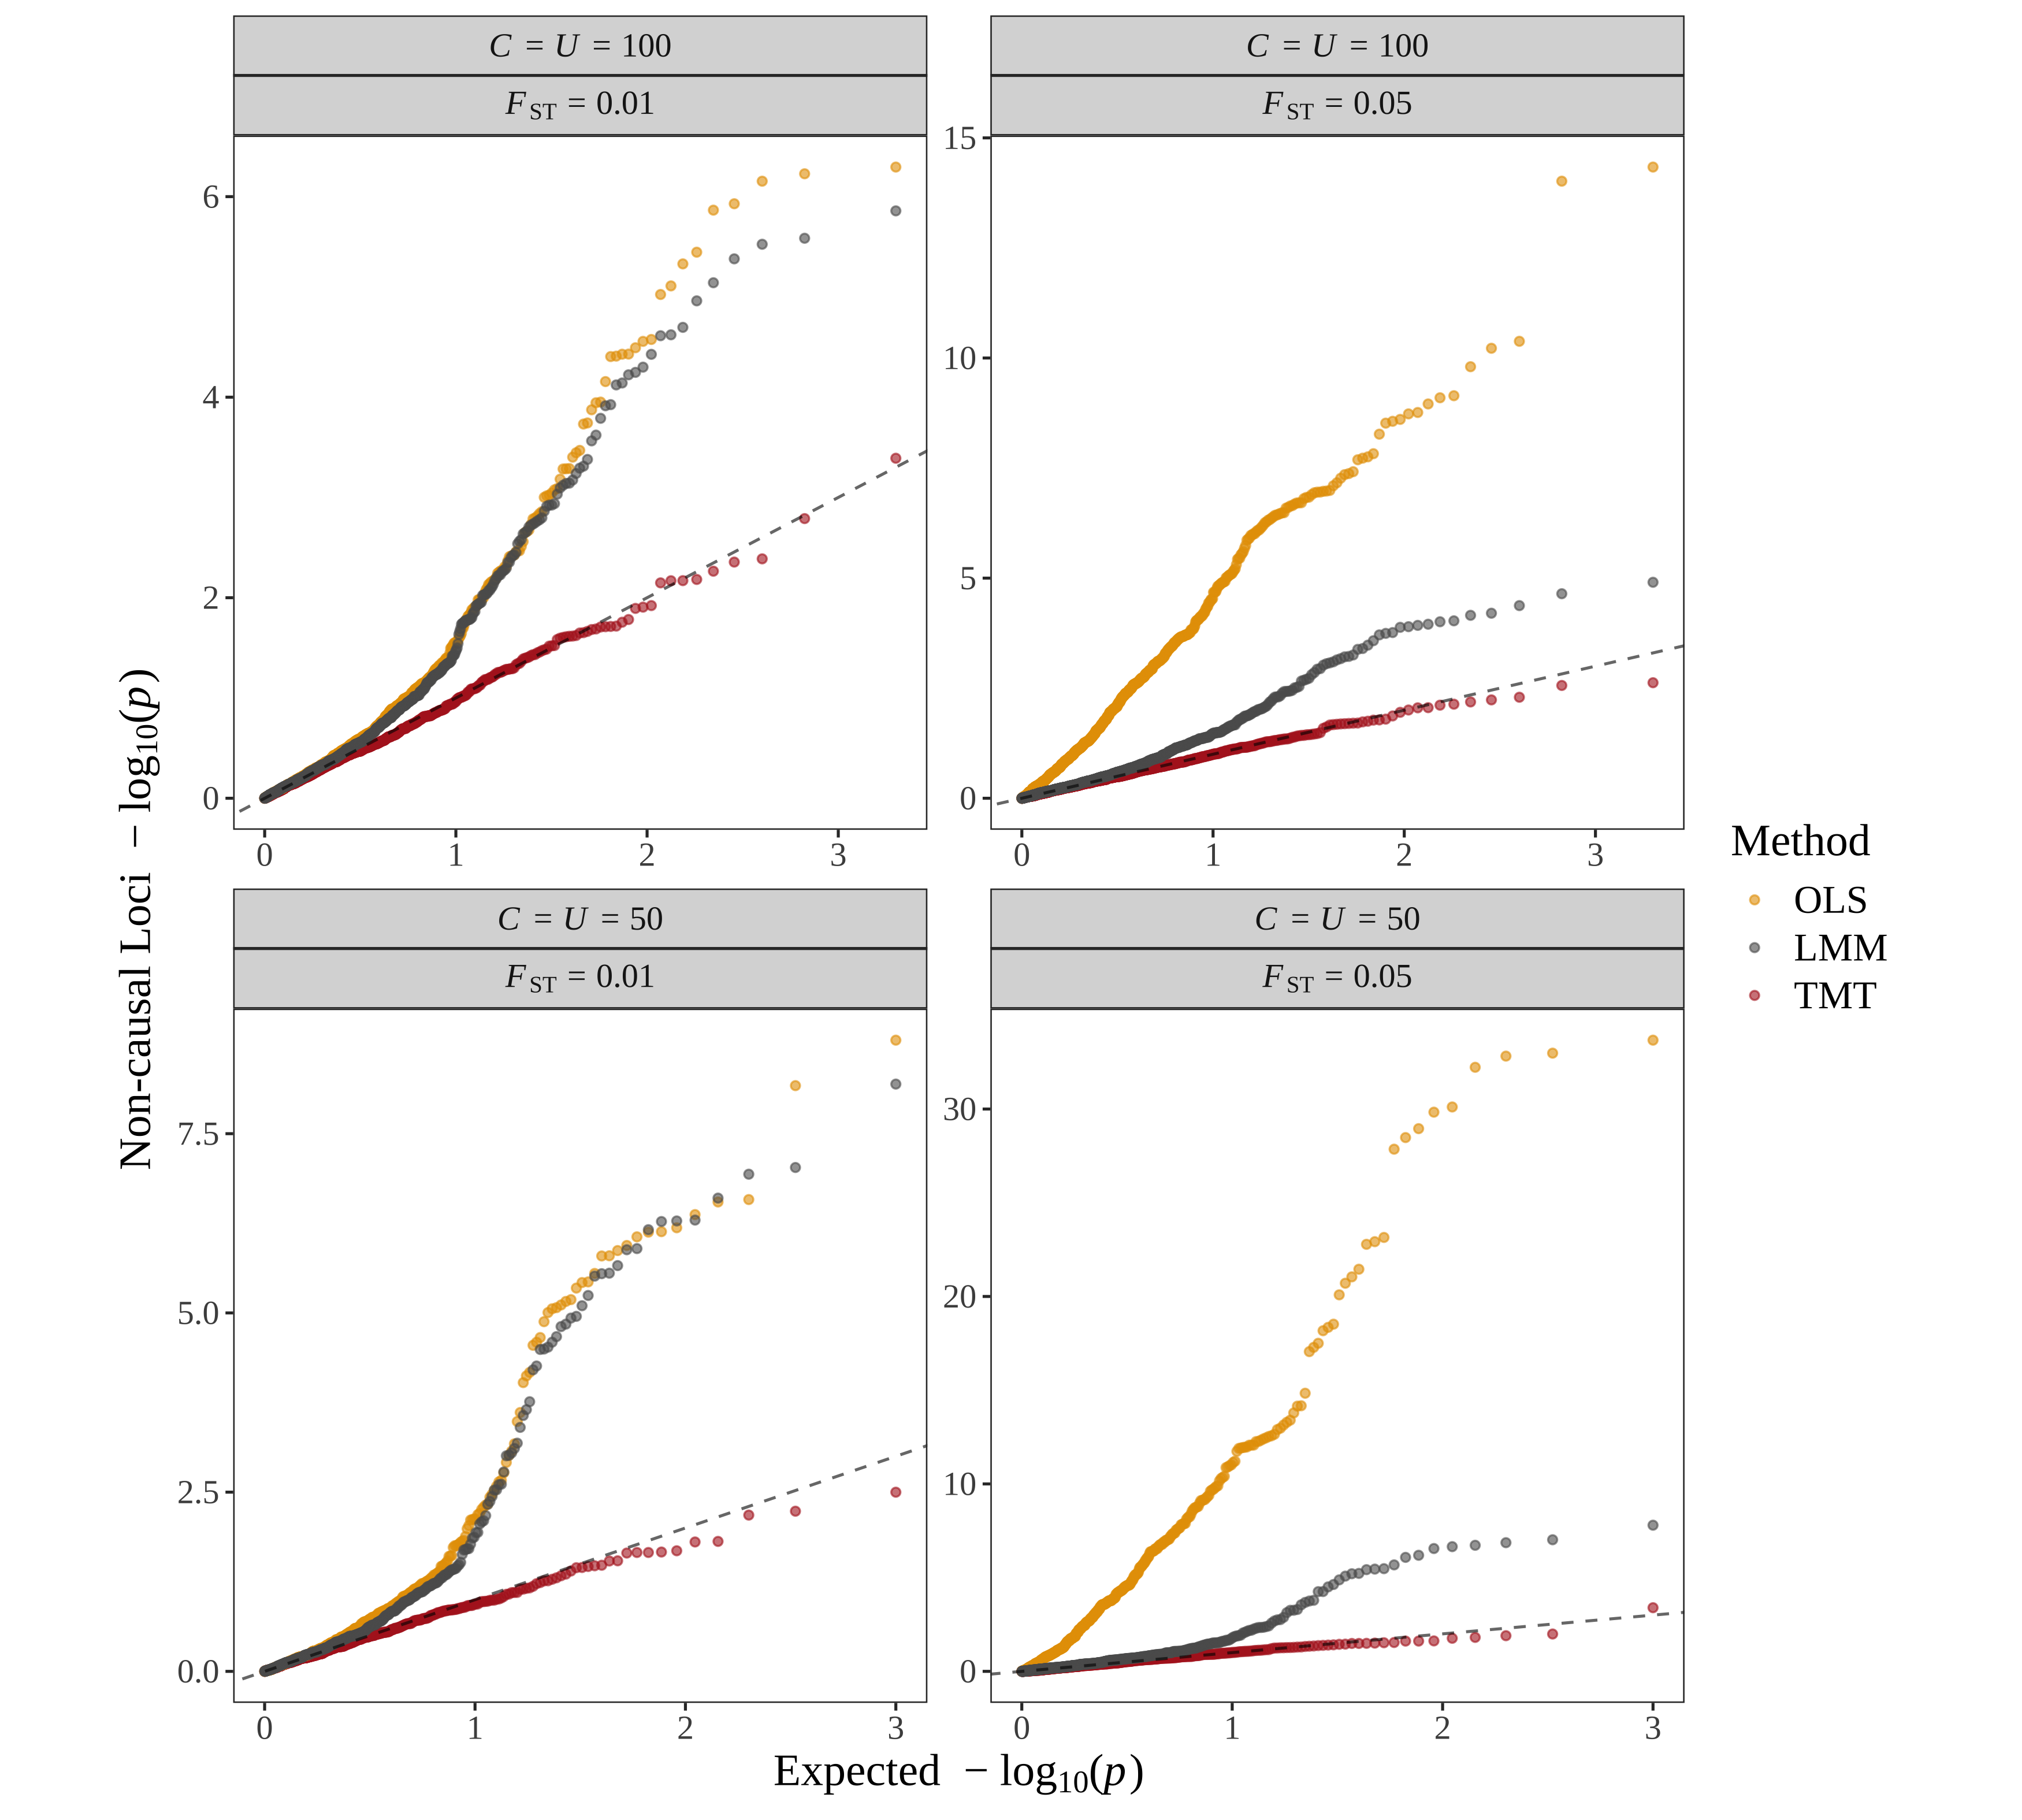
\includegraphics[clip, trim=0cm 0cm 0cm 0cm, width = 1\textwidth]{./figures/figure6.png} % trim by left botm right top
\caption{\textbf{The distribution of $-\log_{10}$($p$) at non-causal SNPs by the ordinary least square (OLS), the linear mixed model (LMM) and the TMT.} The expected $p$-values on the x-axis are drawn from Uniform(0,1). Points are sorted by their quantiles.}
\label{fig:tmt_lmm}
\end{figure} 

To assess the behavior of the TMT, OLS, and LMM approaches in the presence of exogeneity, for each child $j \in [1:J]$, we generated traits according to
\begin{align*}
Y_j &= \intercept + \sum_{i\in \cC} b_i G_{ij} + \kappa_j + \epsilon_j,
\end{align*}
where $\cC$ is the set of causal SNPs and $\kappa_j$ is confounded with a subset of non-causal (and unassociated) SNPs.  Full details are in \Cref{app:simulate_confounding}.  We implemented the TMT on a per marker basis to detect causal genotypes. We employed the LMM software \texttt{GCTA} \citep{yang2011} to detect associations. We also conducted simple linear regression between child trait and child genotypes on a per locus basis to test associations via OLS. In our simulation, the only SNPs that are associated with the trait are causal SNPs. Let $C$ be the total number of causal SNPs and $U$ the total number of non-causal confounded SNPs. \Cref{fig:tmt_lmm} displays the distribution of $p$-values at non-causal SNPs where we induced confounding and $9U$ other random non-causal and unconfounded SNPs. Since these $10U$ SNPs are non-causal (and unassociated with the trait), their $p$-values should be Uniform$(0,1)$ distributed. In our simulations, only the TMT results in Uniform$(0, 1)$ distributed $p$-values of non-causal SNPs. Both LMM and OLS report significantly small $p$-values deviating from Uniform$(0, 1)$ for non-causal SNPs.

%\subsection{TMT avoids spurious associations compared to linear regression} \label{sec:result_mmam}
%
%The TMT and TDT are approaches with some key differences compared to established GWAS methods. Here, we are assuming that traits are measured only on the children. Given this, it is possible to ignore the parental genotypes and simply perform a standard GWAS analysis on the children. We compare the TMT and TDT to these methods to understand the advantages and disadvantages, as well as how the two approaches can be used together. We employ three established GWAS methods including (i) the simple linear regression (SLR) between the trait and every single SNP \citep{plink2007}, (ii) the linear mixed-model (LMM) for quantitative trait association analysis \citep{kang2010, yang2010,yang2011}, (iii) the generalized linear mixed-model (GLMM) for binary trait association analysis \citep{chen2016}, and (iv) the genotype-conditional association test (GCATest) \citep{song2015}. 
%
%\begin{figure}[htbp] %  figure placement: here, top, bottom, or page
%   \centering
%   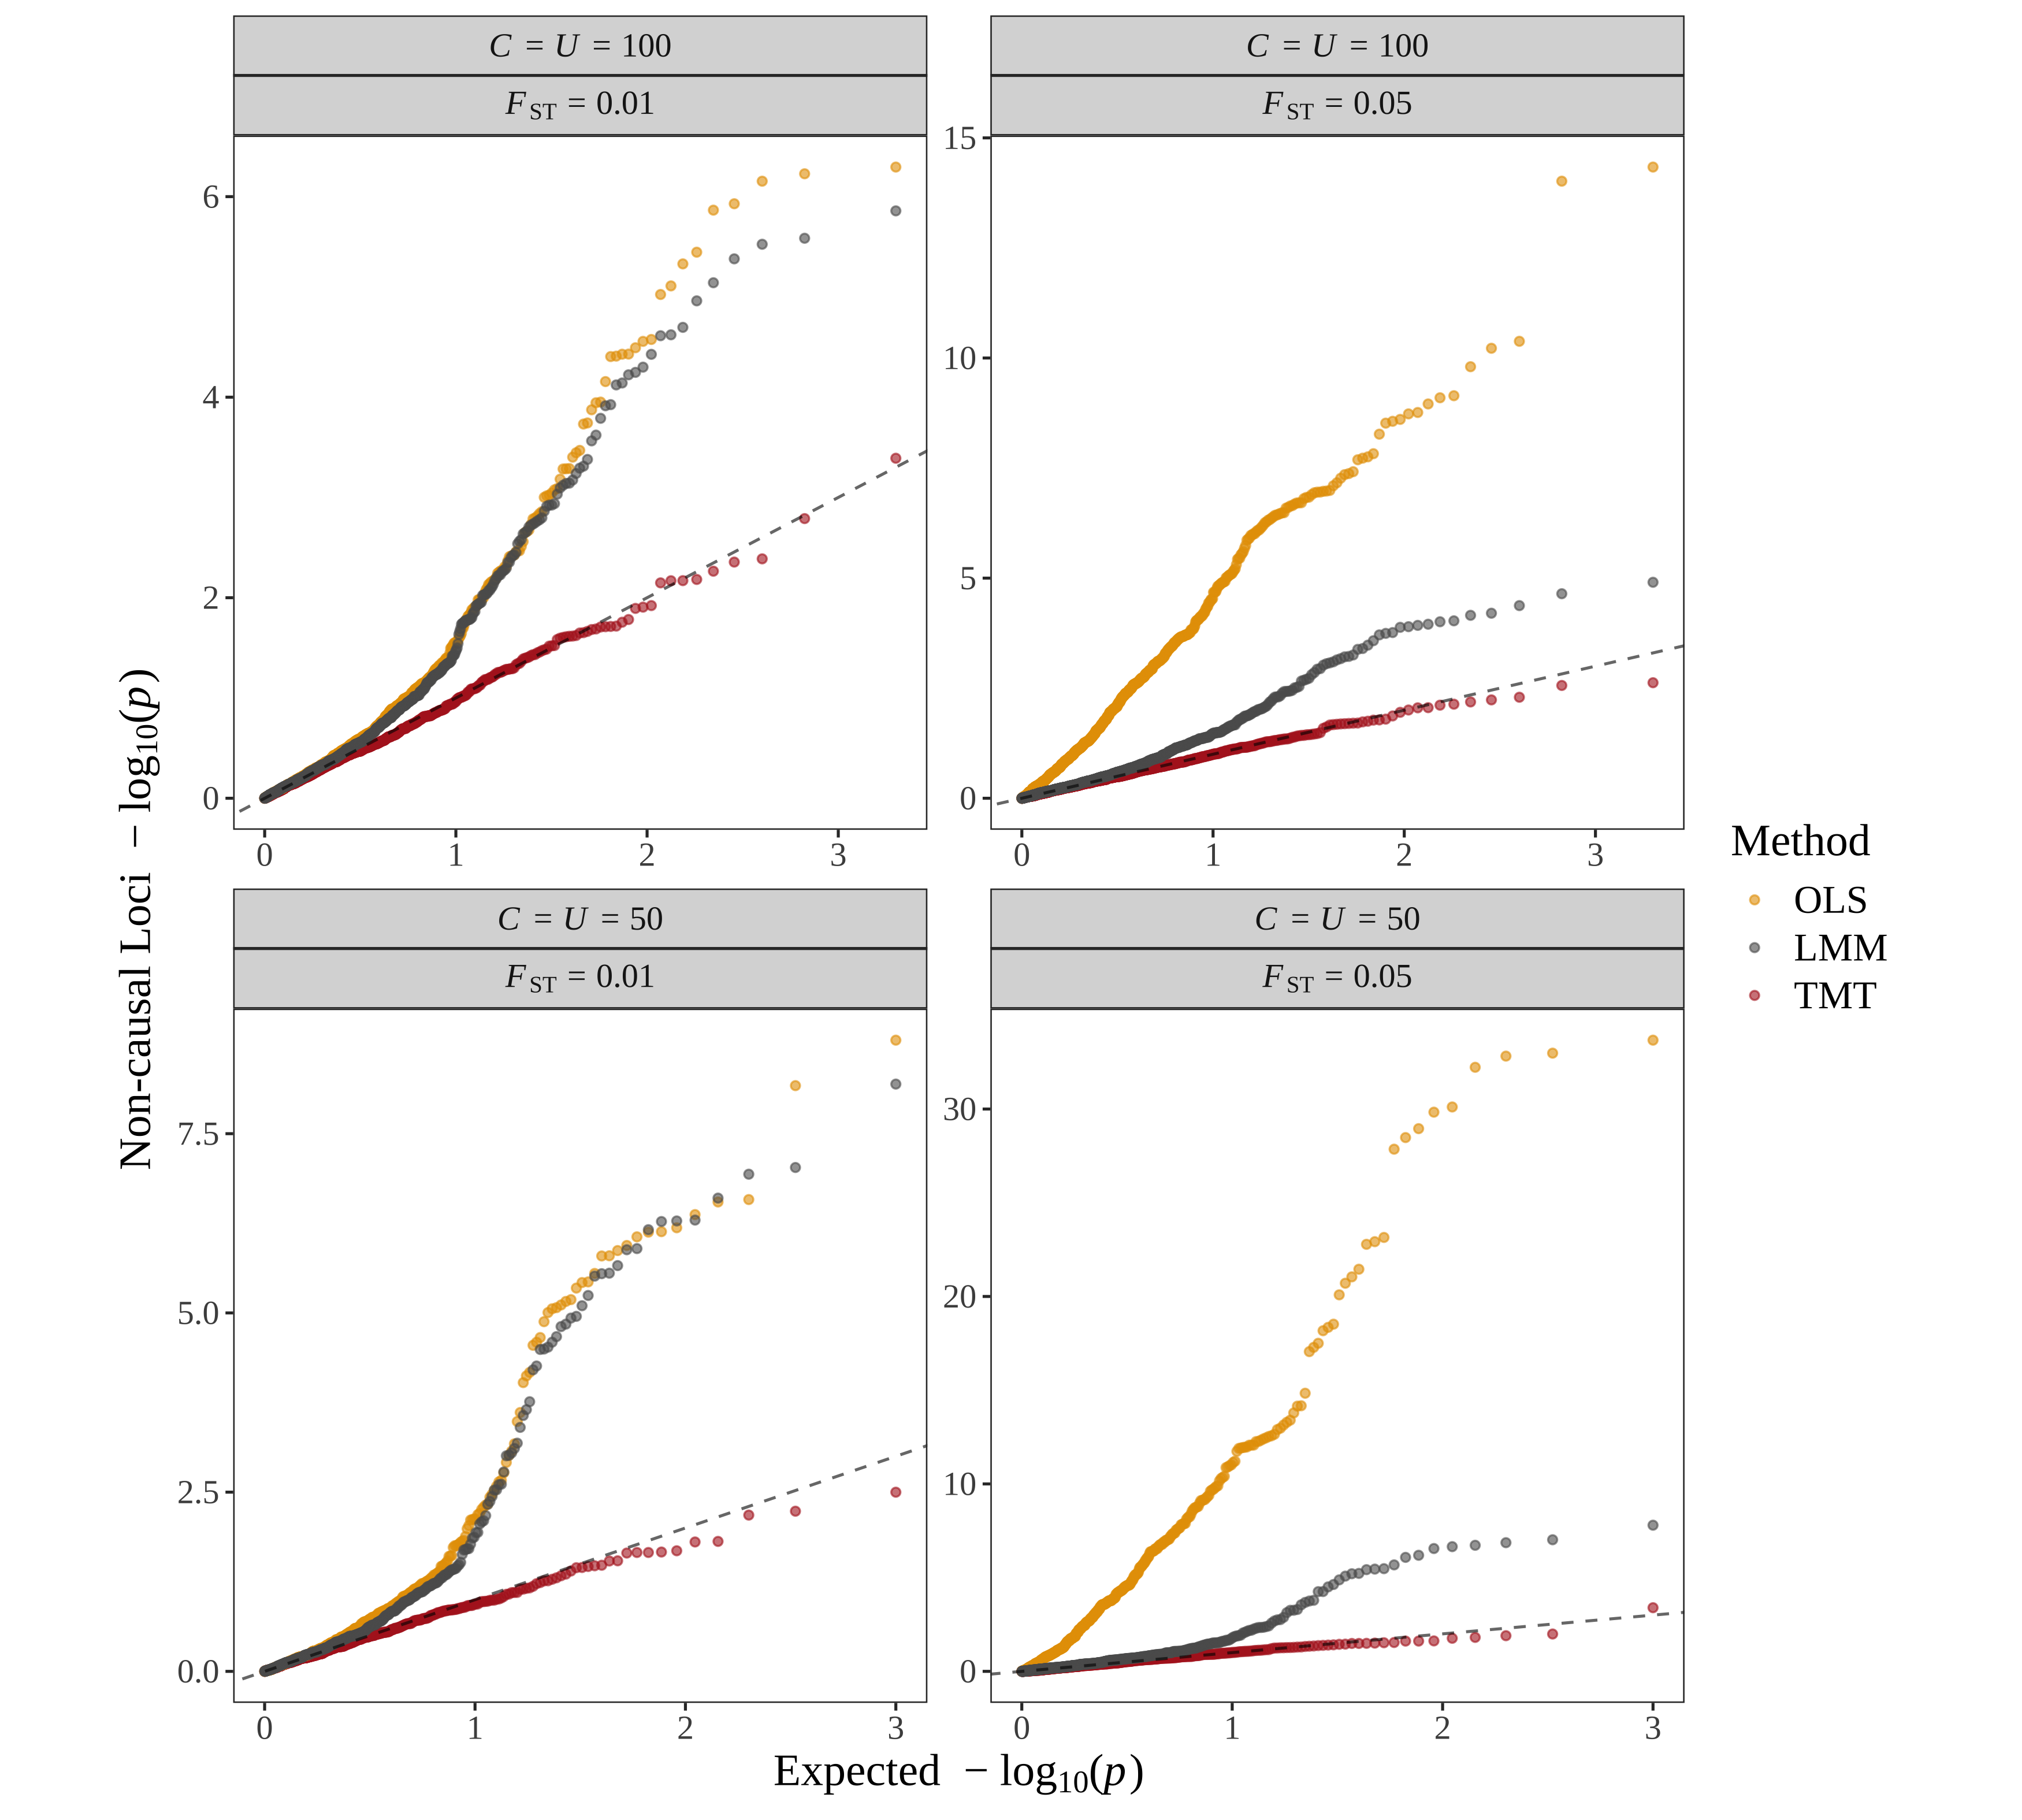
\includegraphics[clip, trim=0cm 0cm 0cm 0cm, width = 0.9\textwidth]{./figures/figure6.png} % trim by left botm right top
%   \caption{\textbf{Comparisons of TMT to established association methods. (A)} Observed false positive rate (FPR) vs expected FPR for simulated quantitative traits. \textbf{(B)} The area under the ROC curve for simulated quantitative traits.\textbf{(C)} Observed FPR vs expected FPR for simulated binary traits. \textbf{(D)} The area under the ROC curve for simulated binary traits. (A) and (C) are results of a randomly chosen simulated data set. The true $h^2$ in (A) and (C) is 0.5 but choosing other levels of desired $h^2$ produced similar results. Each box in (B) and (D) contains results for 100 simulated data sets.}
%   \label{fig:tmt_assoc}
%\end{figure}
%
%In general, the SLR does not account for population structure, which leads to false positives. The TMT and the TDT are immune to these false positives due to the randomization via conditioning on parental genotypes. Other methods control or avoid these false positives via different approaches. The LMM and the GLMM approaches utilize an estimated covariance model that takes into account population structure as measured by kinship and the polygenic background. The GCATest performs an inverse regression of genotype on trait, conditional on individual-specific allele frequencies based on a model of structure. GCATest is also robust to the polygenic background and also has theoretical guarantees that it accounts for structure. 
%
%We implemented simulations to compare the methods. For quantitative traits, we followed \Cref{app:sim_trio_geno} to simulate 5,000 trios with 100,000 SNPs per individual and used \Cref{eq:ptm_with_e} to generate child traits with 100 directly causal loci across various levels of desired heritability. For each SNP, we conducted a causal test via the TMT and association tests via the SLR, the LMM by software \texttt{GCTA} \citep{yang2011}, and the GCATest. The SLR fails to remove spurious associations and false positives, as expected (\Cref{fig:tmt_assoc}A). When the true heritability is not extremely low, the TMT, LMM, and GCATest have high area under the ROC values while the SLR does not (\Cref{fig:tmt_assoc}B). 
%
%When the true genetic effect sizes are small, making the true $h^2$ low, the LMM and GCATest obtain higher values of the area under the ROC curve than the TMT. because the trait simulation process completely satisfies the polygenic trait model assumptions in LMM. Besides, the GCATest delivers very good identifications of non-zero genetic effect sizes since the latent variables are sufficient enough to capture characteristics of the individual allele frequencies. This is guaranteed by choosing an ideal number of latent variables to be modeled, which is at least four in our simulations as we have drawn samples from four intermediate subpopulations. The LMM requires more restrictive assumptions for the trait variance components, which are also strictly satisfied in our simulations and further ensured by our consistent kinship estimation approach \citep{ochoa2021} so that the LMM almost removes the heterogeneity in the individual allele frequency, yielding an association test result that is comparable to the causal inference result by the TMT. Violating these trait variance components assumptions can decrease the power of the LMM without observable influences on the TMT and GCATest, which will be discussed in \Cref{sec:tmt_lmm}. 
%
%For binary traits, we followed \Cref{sec:tdt_empirical} to generate 5,000 trios with affected children and 5,000 trios with normal children, with 100,000 SNPs per individual. We conducted the TDT for the 5,000 affected-only trios and we implemented the other methods, including the TMT, SLR, and GCATest, for 5,000 randomly chosen trios composed of an equal number of affected and normal children . The SLR is still the only one that performs similar to a random classification (\Cref{fig:tmt_assoc}C and D). We did not implement the GLM for the above set of experiments because it would require extremely cumbersome computation. Instead, we carried out another set of experiments with similar study design but smaller sample size while implementing the GLM by the R package \texttt{GMMAT} \citep{chen2016} to compare the GLM with other methods (\Cref{fig:tdt_assoc}). The GLM by \texttt{GMMAT} and the GCATest provide comparable associations diagnoses for binary traits, whose accuracy is a natural result due to the trait simulations satisfying assumptions of GLM. These assumptions may be violated in a particular clinical study, such as the ascertained case-control studies in \Cref{sec:tmt_lmm}, where the TDT and the TMT would find promising applications.
%
%
%\subsection{TMT is robust to scenarios where the mixed-model assumptions are violated} \label{sec:tmt_lmm}
%
%\paragraph{Linkage disequilibrium between directly causal loci.}
%
%LMM assumes linkage equilibrium between loci under investigations. If a considerable proportion of directly causal loci are in linkage with each other, LMM would encounter a potential restriction of the statistical power because loci under test and their linked loci are treated as both fixed effects for the association test and also random effects for genetic relatedness measurement \citep{listgarten2012, yang2014}. In contrast, the TMT retains the statistical power because it does not necessarily require the linkage equilibrium assumption. 
%
%\begin{figure}[htbp] %  figure placement: here, top, bottom, or page
%   \centering
%   \includegraphics[clip, trim=2cm 22cm 2cm 18cm, width = 1\textwidth]{./figures/figure7.png} % trim by left botm right top
%   \caption{\textbf{Methods performances comparison when directly causal loci are linked. (A)} Changes of the average negative $\log_{10}(p$-value$)$ across causal loci as the percentage of linked loci increases. Each box plot contains results of 100 simulations for 5,000 trios out of a structured population ($F_{ST}=0.2$), 100,000 SNPs per individual, and 1,000 causal loci. \textbf{(B)} The area under the precision-recall curve for three methods.}
%   \label{fig:tmt_mmam_ld}
%\end{figure}
%
%We examined the above analysis by simulating various levels of genetic linkage between 1,000 directly causal loci among 5,000 trios with 100,000 SNPs per individual (\Cref{fig:tmt_mmam_ld}). Among these 1,000 directly causal loci, we randomly selected $c$ central SNPs with $v$ nearby linked loci per center such that $c \times v$ is as close to 1,000 as possible. Let $v/100,000 \times 100\%$ be the linked loci percentage out of all 100,000 simulated SNPs. We reported the average negative $\log_{10}(p$-values$)$ across 1,000 causal loci by the LMM, the GCATest and the TMT (\Cref{fig:tmt_mmam_ld}A). As the linked loci percentage increases, the number of highly positively correlated SNPs increases so that a directly causal locus enhances its trait contribution through its correlated SNPs besides their single-loci direct contributions, and thereby, anticipating a higher negative $\log_{10}(p$-values$)$ per causal loci. This expectation has been met by the GCATest and the TMT but not the LMM. The LMM even generates descending average negative $\log_{10}(p$-values$)$ as the linked loci percentage increases and passes a certain threshold, which leads to a decreasing trend of the area under the precision-recall curve (auPRC) while the other two methods retain high values of auPRC (\Cref{fig:tmt_mmam_ld}B). These patterns validate our analysis about the failure to retain power when using the LMM while loci under test are repeatedly treated as both fixed effects for the association test and random effects for kinship estimation. Although this problem may be overcome if excluding loci under test and its linked ones from kinship calculation, such correction requires a new round of kinship estimation per locus association test, which would introduce unrealistic computation burden to the biobank-scale data with millions of SNPs and render the GCATest and the TMT as more reasonable approaches. 
%
%
%\paragraph{Ascertained case-control studies.}
%
%Both LMM and GLM have a restrictive assumption about the trait's variance-covariance structure. For a quantitative trait, the LMM assumes a multivariate normal distribution with a particular variance-covariance structure $2\sigma_a^2\boldsymbol{\Phi}+\sigma_e^2\mathbb{I}$, where $\boldsymbol{\Phi}$ denotes the kinship matrix, $\mathbb{I}$ the identity matrix, $\sigma_a^2$ the genetic variance, and $\sigma_e^2$ the environmental variance. For a binary trait, the GLM assumes a similar variance-covariance structure after transforming the trait via a logit or probit function. One guarantee for this assumption is that individuals are randomly sampled so that the sampling procedure is independent of the phenotype. However, clinic case-control studies usually ascertain more cases than the expected disease prevalence to increase the statistical power. In such a scenario, previous works have reported loss of power when using LMM and GLM \citep{yang2014, weissbrod2015, hayeck2015} but have not elucidated the reason. One possible reason is that the case ascertainment introduces mismatch between the expected and observed values of the variance components. This hypothesis is now testable by using the TMT and the GCATest to set up a synthetic control, since the TMT and the GCATest do not require the restrictive assumption about trait variance components.
%
%\begin{figure}[htbp] %  figure placement: here, top, bottom, or page
%   \centering
%   \includegraphics[clip, trim=2cm 15cm 2cm 5cm, width = 1\textwidth]{./figures/figure8.png} % trim by left botm right top
%   \caption{\textbf{Methods performances comparisons in ascertained case-control studies. (A)} The average negative $\log_{10}(p)$-values at causal loci by the GCATest, LMM, and TMT. The ``Origin'' on the x-axis denotes no ascertainment. Each box contains results of 30 simulations for 5,000 trios from a structured population ($F_{ST}=0.2$), 10,000 SNPs per individual, and 100 causal loci. For each disease prevalence, we report average negative $\log_{10}(p$-value$)$ across all causal loci. The desired heritability is 0.5. \textbf{(B)} The residual variance generated by fitting LMM via \texttt{GCTA}. The gray dashed line marks the true value $\sigma_e^2=1$. \textbf{(C)} The distribution of residuals ${\hat{\epsilon}_j}$ generated by LMM, with the mean value deviating away from zero as the disease frequency decreases.}
%   \label{fig:tmt_lmm_acc}
%\end{figure}
%
%We simulated ascertained case-control trios to examine the above hypothesis. Our sample contains 5,000 trios with a 1:1 case-control ratio across various values of the disease prevalence. Specifically, we first followed \Cref{app:sim_trio_geno} to simulate 150,000 trios genotypes and the child phenotype $\boldsymbol{Y}=\{Y_j\}$ by $Y_j= \intercept + \sum_{i\in \cC}\beta_cG_{ij} + \epsilon_j$ with the desired heritability $h^2=\sigma_a^2/(\sigma_a^2+\sigma_e^2)=0.5$ where $\sigma_e^2=\sigma_a^2=1$, $\epsilon_j \sim N(0,\sigma_e^2)$, and $\cC$ denotes the indices set of causal loci. We set the same value $\beta_c$ as the effect size for all causal loci such that $\sigma_a^2=2\sum_{i\in \cC}\beta_c^2p_i^T(1-p_i^T)$. Per disease prevalence $\lambda$, $\lambda \in \{0.1, 0.01,0.001,0.0001,0.00001\}$, we followed a probit model to identify affected children as cases (details in \Cref{app:simulate_acc_trios}). Let $n^{\ast}$ be the total number of such cases. Among the remaining children, we randomly selected $n^{\ast}$ children into the control group so that the case-control ration is ascertained to 1:1. We repeated the above procedure until 2,500 cases and 2,500 controls were assembled. We then carried out the GCATest, the LMM, and the TMT to test significant genetic effect sizes. Let $\{\hat{\beta}_i\}$ be the best linear unbiased estimates (BLUE) of genetic effect sizes by the LMM. We computed the LMM fitted residual $\{\hat{\epsilon}_j\}$ by $\hat{\epsilon}_j=Y_j - \intercept -\sum_{i \in \cC}\hat{\beta}_iG_{ij}$, together with its observed variance $\text{Var}(\hat{\epsilon}_j)$. 
%
%We compared the statistical power of the GCATest, the LMM, and the TMT by reporting their average negative $\log_{10}$($p$-values) at the causal loci (\Cref{fig:tmt_lmm_acc}A). For small values of disease prevalence (less than 0.05\%), the LMM is less sensitive to directly causal effects than the TMT. This is because the case ascertainment has introduced a difference between the observed variance of the LMM residual $\text{Var}(\hat{\epsilon}_j)$ and the true variance value $\sigma_e^2$ (\Cref{fig:tmt_lmm_acc}B). The difference $\text{Var}(\hat{\epsilon}_j)-{\sigma}_e^2$ becomes larger for a smaller value of the disease prevalence. The LMM residual distribution is shifted away from $\mathcal{N}(0,\sigma_e^2)$ under ascertainment (\Cref{fig:tmt_lmm_acc}C), violating the LMM assumption about the trait variance-covariance structure. This is not a concern for the GCATest and the TMT as they do not require such restrictive assumption about the variance-covariance structure.

\subsection{Applying the TMT to large-scale association studies} \label{sec:biobank}

Large-scale studies, such as the UK Biobank \citep{bycroft2018} and \textit{All of Us} \citep{allofus2024}, involve hundreds of thousands of individuals. Many of the individuals in such large studies may be closely related. When studies contain closely related individuals (e.g., parent-child trios), researchers often retain only one of these individuals and exclude the others from the GWAS analysis. With the proposed TMT framework, one can instead set all closely related individuals aside and perform the GWAS on the remaining individuals. One can then follow up by validating the associations for causal effects on the related individuals using the TMT. Since the closely related individuals were not included in the initial GWAS analysis, one can even focus on a smaller set of the most significant SNPs from the GWAS analysis.

The UK Biobank has reported 107,162 related pairs (third degree or closer) \citep{bycroft2018} by examining kinship coefficients estimated with the software \texttt{KING} \citep{manichaikul2010} and discordant homozygote rates. Following the criteria from \texttt{KING}, we extracted individual pairs with kinship estimates around 1/4 (between $2^{-5/2}$ and $2^{-3/2}$) as first degree relatives but not monozygotic twins. We further filtered out individual pairs with a discordant homozygote rate greater than 0.1, which are likely  to be siblings. We classified the remaining individual pairs as parent-offspring pairs and identified families with at least one child and two parents (one male and one female). Through this procedure we identified 1,970 trio candidates, similar to previous studies \citep{bycroft2018,browning2022}. These sample sizes have reasonable power as shown in our simulations, especially on a well-selected subset of SNPs identified in a traditional GWAS as causal candidates. We expect a comparable or larger sample size of parent-child trios for the \textit{All of Us} data since it has reported a much larger size of closely related participants, specifically 215,107 pairs (second degree or closer) \citep{allofus2024}. 

As evidenced by the thousands of citations of the original TDT publications \cite{terwilliger1992, spielman1993, ewens1995}, trio studies play an important role in genetics. In dbGaP, trio studies with reasonable sample sizes are available, presenting both whole-genome sequencing data and phenotypes of interest. For example, the Pediatric Cardiac Genetics Consortium involves more than 5,000 trios, together with a disease status related to congenital heart disease; it aims to recruit 10,000 trios with affected and unaffected children \citep{pcgc2013, jin2017}. The total number of trios in these studies have similar sample sizes to our simulations. Therefore, in addition to the large-scale studies containing many trios, the proposed methods should be useful to apply to existing and forthcoming studies aimed at directly sampling trios.

% Comparing to the LMM and GLM, the TMT and the TDT are easier to be scaled to the aforementioned biobank-level data. Consider a study cohort of $\nind$ children with $\nsnp$ loci per individual. For quantitative traits, the LMM requires at least a sum of $O(\nsnp \nind^2)$ for kinship estimation, $O(\nind^3)$ for variance components estimations, and $O(\nsnp \nind^2)$ for association test \citep{yang2014}. Binary trait analysis with the GLM has a much severer computational complexity issue since the likelihood function is usually not tractable which requires multiple rounds of approximations additionally \citep{chen2016}. In contrast, the TMT and the TDT have the complexity of $O(\nsnp \nind)$, making it much more computationally efficient than the LMM and the GLM. 


\section{Discussion}\label{sec:discussion_mendel}

%What is TMT / TDT
%What did we show
%Vision of where to apply it
%Strengths
%Weaknesses
%Future work

In studies where genetic trios (two parents and a child) are sampled from a population, it is possible to measure the transmission of genetic variants from parent to child. We have shown that by leveraging the inherent randomization in this process, it is possible to construct a potential outcomes model and inference method to rigorously test for causality from genetic variant to trait in the child. We proposed the transmission mean test (TMT) in this scenario for all common trait types -- quantitative, count, or dichotomous. We showed that within our framework, the well-known transmission disequilibrium test (TDT), where trios are sampled based on a dichotomous affected trait status in the child, is also a test of causality.

We demonstrated both theoretically and empirically that the TMT and TDT are robust to a wide range of confounders, including population structure and the confounding of non-genetic variation with the genetic signal. Our theoretical analysis showed how genetic relatedness and structure of parents within and between trios do not affect the accuracy of our tests. More generally, our theoretical results clarify why the analysis of the concordance of genetic transmission and traits within and among many pedigrees is robust to common confounders. We showed how linkage disequilibrium and meiotic genetic linkage play roles in shared signal among neighboring SNPs. 

The proposed framework is based on the potential outcomes model of causality in the context of randomized studies, which is the gold standard used in randomized controlled clinical trials required by the FDA \citep{fda1998}. Mendelian randomization is a method applied to standard GWAS where unrelated individuals from a population are sampled. Despite its name, Mendelian randomization does not observe the randomization process of genetic inheritance from parent to child. Rather, it is a method that implements instrumental variable regression using a genotype as the instrument. Mendelian randomization requires several assumptions, including no population structure \citep{bochud2008}. A framework exists for the scenario where both parents and the child have phased genomes that utilizes a probabilistic independence definition of causality \citep{pearl2009} and a computationally intensive simulation based null distribution \citep{bates2020}, requiring Haldane's model of recombination \citep{lange2002}. 

Given that standard GWAS can have very large sample sizes, one may consider the relevance of trio based studies. We noted that many trio studies of a reasonable sample size are present in dbGaP. We also discussed that large studies, such as the UK Biobank \citep{bycroft2018} and \textit{All of Us} \citep{allofus2024},  contain many instances of first degree relatives, including full parent-child trios. A possible strategy is to set aside the first degree relatives and perform a standard GWAS on the remaining individuals to identify causal candidates based on associations. One can then employ the TMT on the related individuals on a reduced set of candidate SNPs to identify causal variants.  Going beyond trios to more general first degree relatives, such as siblings, future work could develop a framework where one can first predict missing parental genotypes by Mendelian imputation \citep{young2022} and then conduct the TMT based on this probabilistic imputation.

%Conditioning on the parental genotypes, the transmission-based methods deliver a causal inference framework that prevents false positives and false negatives in the presence of population structure, non-genetic factors confounded with population structure, linkage disequilibrium, and case ascertainment. The TMT and the TDT are applicable to most parent-child trio study designs. 
%
%Focusing on the theories, the current work does not involve real phenotype data but we anticipate no pains when implementing the algorithm since the transmission-based methods are likelihood-free and have linear complexity.

%A related but distinct line of work is referred to as \textit{Mendelian randomization} \citep{davey2003, lawlor2008, bochud2008, vanderweele2014}. Technically accurate terminology for this type of methods is \textit{genetic instrumental variable} since they use genetic variability as an instrumental variable to identify non-genetic factors that are causal for phenotypes of interest. As relationships between genes and phenotypes are not of primary interest of the approach of genetic instrumental variable, Mendelian randomization may be a misnomer. On the other hand, we note that transmission-based methods actually implement Mendelian randomization as their validity justified by the meiotic process as a source of experimental randomization.

%We compared the TMT and the TDT with existing association methods for phenotype-genotype relationship analysis. Besides, a philosophical difference is that the TMT and the TDT indeed implement randomization while association methods do not. As FDA recommends randomization as a normal feature of clinical trials and drug development \citep{fda1998}, it is worthwhile to consider the TMT and the TDT besides association methods to guarantee the accuracy of treatment effect evaluations.

%While the merits of parent-child trio data are significant, one clear disadvantage to trio-based methodologies is the difficulty of data acquisition. Recruiting entire families into studies, rather than just individuals, often hinders the acquisition of large-scale datasets. One circumstance in which collecting trio data is natural is in the study of childhood disease. In this setting, parents and children are simultaneously recruited to a study during hospital visits. This type of sampling strategy is appropriate for the TDT, which, in part, explains the popularity of the TDT. However, with the continuously declining cost of genetic sequencing, it is plausible that trio-data will soon be available for entire, defined populations of interest. This may occur even for datasets that do not explicitly familial relationships. In a large enough sample, trio relationships are expected to naturally occur. Furthermore, trio relationships can be identified from genetic information alone, as we have shown for the UK Biobank data in \Cref{sec:biobank}. Some studies may only have genotyped a part of family members but not the whole. In that case, one can first predict missing genotypes by a recently developed technique named Mendelian imputation \citep{young2022} and then conduct the TMT. This strategy motivates future research of extending the TMT framework for data on two or more first degree relatives. 

\subsection*{Resources}

Reproducible research documentation is available at \url{https://github.com/StoreyLab/causal-trio}. An R package \texttt{geneticTMT} that implements the proposed methods is available at \url{https://github.com/StoreyLab/geneticTMT}.

\subsection*{Acknowledgments}

This work was supported by US National Institute of Health grant R01 HG006448.

\clearpage
\printbibliography  \addcontentsline{toc}{section}{References}

\clearpage

\appendix

\addtocontents{toc}{\protect\setcounter{tocdepth}{1}}

\section*{Appendices} \addcontentsline{toc}{section}{Appendices}
\section{Theory}

\subsection{Proof of \Cref{lem:gma}} \label{app:gma}

Under the trait model in \Cref{eq:app_gtm},  
\begin{align*}
\ace (A^m \to Y) + \ace (A^p \to Y) &= \E[Y^m(1)]-\E[Y^m(0)] + \E[Y^p(1)]-\E[Y^p(0)]\nonumber \\
&= (\alpha_1-\alpha_0)\pp(A^p=0) + (\alpha_2-\alpha_1)\pp(A^p=1) ~ \nonumber \\
& \qquad + (\alpha_1-\alpha_0)\pp(A^m=0) + (\alpha_2-\alpha_1)\pp(A^m=1).
\end{align*}}Assume $0<\pp(A^m=1)<1$ and $0<\pp(A^p=1)<1$. Under \Cref{asm:genetic_model}, either $\alpha_0\leq \alpha_1 \leq \alpha_2$ or $\alpha_0\geq \alpha_1 \geq \alpha_2$. Then $\ace (A^m \to Y) + \ace (A^p \to Y)=0$ if and only if $\alpha_0\neq \alpha_1$ or $\alpha_1\neq \alpha_2$, which means $\ace(G\to Y) \neq 0$ by \Cref{def:ace_genotype}. 

\subsection{Proof of \Cref{lem:law_segregation}} \label{app:cind}

Here we show $\Big(Y^m(0),Y^m(1)\Big)\ind A^m | Z^m=1$. The proof for $\Big(Y^p(0),Y^p(1)\Big)\ind A^p | Z^p=1$ is the same. We first show that $A^p \ind A^m |Z^m=1$ through several calculations. 
{\allowdisplaybreaks 
\begin{align}
& ~~~~ \cV(A^m,A^p|Z^m=1) \nonumber \\
&= \E[A^m A^p|Z^m=1] - \E[A^m|Z^m=1]\E[A^p|Z^m=1] \nonumber \\
&= \pp(A^m=1,A^p=1|Z^m=1) - \pp(A^m=1|Z^m=1) \pp(A^p=1|Z^m=1) \nonumber \\
&= \pp(A^m=1|Z^m=1)\pp(A^p=1|A^m=1,Z^m=1) - \frac{1}{2}\pp(A^p=1|Z^m=1) \nonumber \\
&= \frac{1}{2}\pp(A^p=1|A^m=1,Z^m=1) - \frac{1}{2}\pp(A^p=1|Z^m=1). \tag{A2.a} \label{eq:a2a} 
\end{align}}
By the Law of Total Covariance,
{\allowdisplaybreaks 
\begin{align}
& ~~~~ \cV(A^m,A^p|Z^m=1)  \nonumber \\
&= \E\Big[\cV(A^m,A^p|Z^m=1,Z^p=1)\Big|Z^m=1\Big] \nonumber \\
& \qquad \qquad + \cV\Big(\E[A^m|Z^m=1,Z^p=1],\E[A^p|Z^m=1,Z^p=1]\Big|Z^m=1\Big) \nonumber \\
&= \E\Big[\E[A^mA^p|Z^m=1,Z^p=1]-\E[A^m|Z^m=1,Z^p=1]\E[A^p|Z^m=1,Z^p=1]\Big|Z^m=1\Big] \nonumber \\ 
& \qquad \qquad + \underbrace{\cV\Big(\frac{1}{2},\frac{1}{2}\Big|Z^m=1\Big)}_{=0} \nonumber \\
&= \E\Big[\frac{1}{4}-\frac{1}{2}\cdot \frac{1}{2}\Big|Z^m=1\Big] \nonumber \\
&= 0. \tag{A2.b} \label{eq:a2b}
\end{align}}
Since \Cref{eq:a2a} and \Cref{eq:a2b} are equal, this implies $\pp(A^p=1|A^m=1,Z^m=1) - \pp(A^p=1|Z^m=1) = 0$. Similarly, $\pp(A^p=b|A^m=a,Z^m=1) = \pp(A^p=b|Z^m=1)$ for $a,b\in \{0,1\}$. So 
\begin{align}
& A^m \ind A^p |Z^m=1. \tag{A2.c} \label{eq:a2c}
\end{align} 
By \Cref{asm:law_segregation}, 
\begin{align}
\pp(A^m=a|Z^m=1) &= \frac{1}{2}=\pp(A^m=a|Z^m=1,\gamma), \quad a\in \{0,1\}, \tag{A2.d}. \label{eq:a2d}
\end{align} 
Under the trait model in \Cref{eq:app_gtm}, $Y^m(0)$ and $Y^m(1)$ are functions of $A^p$ and $\gamma$. By \Cref{eq:a2c} and \Cref{eq:a2d}, we have shown that $A^p$ and $\gamma$ are independent of $A^m$ conditional on $Z^m=1$. Thus, $\big(Y^m(0),Y^m(1)\big)|Z^m=1$ and $A^m|Z^m=1$ are independent.

% \paragraph{Alternative approach.} We first show that $A^p \ind A^m |Z^m=1$. Notice that $\E[A^m|Z^m=1] = 1/2$ and

% {\allowdisplaybreaks 
% \begin{align*}
% \pp(A^p=1|Z^m=1) &= \pp(A^p=1,A^m=1|Z^m=1) + \pp(A^p=1,A^m=0|Z^m=1) \nonumber \\
% &= \pp(A^m=1|Z^m=1)\pp(A^p=1|A^m=1,Z^m=1) \nonumber \\
% & \qquad \qquad  + \pp(A^m=0|Z^m=1)\pp(A^p=1|A^m=0, Z^m=1) \nonumber \\
% &= \frac{1}{2}\pp(A^p=1|A^m=1,Z^m=1) + \frac{1}{2}\pp(A^p=1|A^m=0,Z^m=1) \nonumber \\
% &= \frac{1}{2}\Big(\pp(A^p=1|A^m=1,Z^m=1) + \pp(A^p=1|A^m=0,Z^m=1)\Big).
% \end{align*}}Let $\lambda = \pp(A^p=1|A^m=1,Z^m=1) + \pp(A^p=1|A^m=0,Z^m=1)$. Then $A^m|Z^m=1$ follows Bernoulli(1/2) while $A^p|Z^m=1$ follows $\text{Bernoulli}(\lambda/2)$ where $\lambda/2$ is not always $1/2$. So $A^p \ind A^m |Z^m=1$. Under the trait model in \Cref{eq:app_gtm}, $Y^m(0)$ and $Y^m(1)$ are functions of $A^p$ and $\gamma$. By \Cref{asm:gamma_z}, $\gamma \ind A^m \big|Z^m=1$. Then $\big(Y^m(0),Y^m(1)\big)|Z^m=1$ are independent of $A^m|Z^m=1$.

\subsection{Proof of \Cref{lem:dtmtnc_unbiased}} \label{app:dtmtnc_unbiased}

{\allowdisplaybreaks 
\begin{align}
& ~~~~ \E[\dtmtnc | N] = \E \left[ \left. \frac{2}{N}\left(\sum_{j=1}^J Y_jW_{1j} - \sum_{j=1}^JY_jW_{0j}\right) \right| N \right] \nonumber \\
\ & = \frac{2}{N} \sum_{j\in \cJ}\E[W_{1j}Y_j|N] - \frac{2}{N}\sum_{j\in \cJ}\E[W_{0j}Y_j|N] \nonumber \\
\ & = \frac{2}{N}\nind \E[W_1Y|N] - \frac{2}{N}\nind \E[W_0Y|N] \nonumber \\
\ &= \frac{2\nind}{N} \E\Big[\indicator(A^m=1,Z^m=1)Y + \indicator(A^p=1,Z^p=1)Y\Big|N\Big] \nonumber \\
\ & \qquad - \frac{2\nind}{N} \E\Big[\indicator(A^m=0,Z^m=1)Y + \indicator(A^p=0,Z^p=1)Y\Big|N\Big] \nonumber \\
\ & = \frac{2\nind}{N} \E\Big[\indicator(A^m=1,Z^m=1)\big(Y^m(0)\indicator(A^m=0)+Y^m(1)\indicator(A^m=1)\big) \Big|N\Big] \nonumber \\ 
\ & \qquad + \frac{2\nind}{N} \E\Big[\indicator(A^p=1,Z^p=1)\big(Y^p(0)\indicator(A^p=0)+Y^p(1)\indicator(A^p=1)\big) \Big|N\Big] \nonumber \\
\ & \qquad - \frac{2\nind}{N} \E\Big[\indicator(A^m=0,Z^m=1)\big(Y^m(0)\indicator(A^m=0)+Y^m(1)\indicator(A^m=1)\big) \Big|N\Big] \nonumber \\
\ & \qquad - \frac{2\nind}{N} \E\Big[\indicator(A^p=0,Z^p=1)\big(Y^p(0)\indicator(A^p=0)+Y^p(1)\indicator(A^p=1)\big) \Big|N\Big] \nonumber \\
\ & = \frac{2\nind}{N} \E\Big[\indicator(A^m=1,Z^m=1)Y^m(1) \Big|N\Big] \nonumber \\ 
\ & \qquad + \frac{2\nind}{N} \E\Big[\indicator(A^p=1,Z^p=1)Y^p(1) \Big|N\Big] \nonumber \\
\ & \qquad - \frac{2\nind}{N} \E\Big[\indicator(A^m=0,Z^m=1)Y^m(0) \Big|N\Big] \nonumber \\
\ & \qquad - \frac{2\nind}{N} \E\Big[\indicator(A^p=0,Z^p=1)Y^p(0) \Big|N\Big] \nonumber \\
\ & = \frac{2\nind}{N} \E\Big[\E\big[\indicator(A^m=1)\indicator(Z^m=1)Y^m(1)\big|Z^m=1, N\big]\Big|N \Big] \nonumber \\
\ & \qquad + \frac{2\nind}{N} \E\Big[\E\big[\indicator(A^p=1)\indicator(Z^p=1)Y^p(1)\big|Z^p=1, N\big]\Big|N \Big] \nonumber \\
\ & \qquad - \frac{2\nind}{N} \E\Big[\E\big[\indicator(A^m=0)\indicator(Z^m=1)Y^m(0)\big|Z^m=1, N\big]\Big|N \Big] \nonumber \\
\ & \qquad - \frac{2\nind}{N} \E\Big[\E\big[\indicator(A^p=0)\indicator(Z^p=1)Y^p(0)\big|Z^p=1, N\big]\Big|N \Big] \nonumber \\
\ & = \frac{2\nind}{N} \E\Big[\indicator(Z^m=1)\E\big[\indicator(A^m=1)Y^m(1)\big|Z^m=1, N\big]\Big|N \Big] \nonumber \\
\ & \qquad + \frac{2\nind}{N} \E\Big[\indicator(Z^p=1)\E\big[\indicator(A^p=1)Y^p(1)\big|Z^p=1, N\big]\Big|N \Big] \nonumber \\
\ & \qquad - \frac{2\nind}{N} \E\Big[\indicator(Z^m=1)\E\big[\indicator(A^m=0)Y^m(0)\big|Z^m=1, N\big]\Big|N \Big] \nonumber \\
\ & \qquad - \frac{2\nind}{N} \E\Big[\indicator(Z^p=1)\E\big[\indicator(A^p=0)Y^p(0)\big|Z^p=1, N\big]\Big|N \Big] \tag{A3.a} \label{eq:a1} \\
\ & = \frac{2\nind}{N} \pp\big(Z^m=1\big|N\big) \E\big[\indicator(A^m=1)Y^m(1)\big|Z^m=1, N\big] \nonumber \\
\ & \qquad + \frac{2\nind}{N} \pp\big(Z^p=1\big|N\big) \E\big[\indicator(A^p=1)Y^p(1)\big|Z^p=1,N\big] \nonumber \\
\ & \qquad - \frac{2\nind}{N} \pp\big(Z^m=1\big|N\big) \E\big[\indicator(A^m=0)Y^m(0)\big|Z^m=1,N\big] \nonumber \\
\ & \qquad - \frac{2\nind}{N} \pp\big(Z^p=1\big|N\big) \E\big[\indicator(A^p=0)Y^p(0)\big|Z^p=1,N\big] \tag{A3.b} \label{eq:a2} \\
\ & = \frac{2\nind}{N} \pp\big(Z^m=1\big|N\big) \E\big[\indicator(A^m=1)\big|Z^m=1,N\big] \E\big[Y^m(1)\big|Z^m=1, N\big] \nonumber \\
\ & \qquad + \frac{2\nind}{N} \pp\big(Z^p=1\big|N\big) \E\big[\indicator(A^p=1)\big|Z^p=1,N\big]\E\big[Y^p(1)\big|Z^p=1,N\big] \nonumber \\
\ & \qquad - \frac{2\nind}{N} \pp\big(Z^m=1\big|N\big) \E\big[\indicator(A^m=0)\big|Z^m=1,N\big]\E\big[Y^m(0)\big|Z^m=1,N\big] \nonumber \\
\ & \qquad - \frac{2\nind}{N} \pp\big(Z^p=1\big|N\big) \E\big[\indicator(A^p=0)\big|Z^p=1,N\big]\E\big[Y^p(0)\big|Z^p=1,N\big] \tag{A3.c} \label{eq:a3} \\
\ & = \frac{2\nind}{N} \pp\big(Z^m=1\big|N\big) \pp\big(A^m=1\big|Z^m=1,N\big) \E\big[Y^m(1)\big|Z^m=1, N\big] \nonumber \\
\ & \qquad + \frac{2\nind}{N} \pp\big(Z^p=1\big|N\big) \pp\big(A^p=1\big|Z^p=1,N\big)\E\big[Y^p(1)\big|Z^p=1,N\big] \nonumber \\
\ & \qquad - \frac{2\nind}{N} \pp\big(Z^m=1\big|N\big) \pp\big(A^m=0\big|Z^m=1,N\big)\E\big[Y^m(0)\big|Z^m=1,N\big] \nonumber \\
\ & \qquad - \frac{2\nind}{N} \pp\big(Z^p=1\big|N\big) \pp\big(A^p=0\big|Z^p=1,N\big)\E\big[Y^p(0)\big|Z^p=1,N\big] \tag{A3.d} \label{eq:a4} \\
\ &= \frac{2\nind}{N}\cdot \frac{N}{2\nind}\cdot \frac{1}{2}\E\big[Y^m(1)\big|Z^m=1,N\big] + \frac{2\nind}{N}\cdot \frac{N}{2\nind}\cdot \frac{1}{2} \E\big[Y^p(1)\big|Z^p=1,N\big] \nonumber \\
\ & \qquad - \frac{2\nind}{N}\cdot \frac{N}{2\nind}\cdot \frac{1}{2}\E\big[Y^m(0)\big|Z^m=1,N\big] - \frac{2\nind}{N}\cdot \frac{N}{2\nind}\cdot \frac{1}{2} \E\big[Y^p(0)\big|Z^p=1,N\big] \tag{A3.e} \label{eq:a5} \\
\ & = \frac{1}{2}\E\big[Y^m(1)-Y^m(0)\big|Z^m=1,N\big]+\frac{1}{2}\E\big[Y^p(1)-Y^p(0)\big|Z^p=1,N\big] \nonumber \\
\ & = \delta_{\tmt}. \nonumber
\end{align}} 
\Cref{eq:a1} is equal to \Cref{eq:a2} by the Law of Total Probability. \Cref{eq:a2} is equal to \Cref{eq:a3} by \Cref{lem:law_segregation} in that $Y(0),Y(1) \ind A \, \big| \, Z=1.$ \Cref{eq:a4} is equal to \Cref{eq:a5} since $\pp(Z^m_j=1 | N) = \pp(Z^p_j=1 | N) = N/(2J)$, which follows because all parents are exchangeable and there are $2J$ parents. 

\subsection{Proof of \Cref{lem:muc} Part A} \label{app:muc_unbiased}

{\allowdisplaybreaks 
\begin{align}
\E[\hat{\mu}_c | N] & = \E \left[ \left. \frac{1}{N}\left(\sum_{j\in \cJ} Y_jW_{1j} + \sum_{j\in \cJ}Y_jW_{0j}\right) \right| N \right] \nonumber \\
\ & = \frac{1}{N}\sum_{j\in \cJ} \E[W_{0j}Y_j|N]+\frac{1}{N}\sum_{j\in \cJ} \E[W_{1j}Y_j|N] \nonumber \\
\ & = \frac{1}{N} \nind \E[W_0Y|N]+\frac{1}{N} \nind \E[W_1Y|N] \nonumber \\
\ & = \frac{\nind}{N} \E\Big[\indicator(A^m=0,Z^m=1)Y + \indicator(A^p=0,Z^p=1)Y\Big|N\Big] \nonumber \\
\ & \qquad + \frac{\nind}{N} \E\Big[\indicator(A^m=1,Z^m=1)Y + \indicator(A^p=1,Z^p=1)Y\Big|N\Big] \nonumber \\
\ & = \frac{\nind}{N} \E\Big[\indicator(A^m=0,Z^m=1)\big(Y^m(0)\indicator(A^m=0)+Y^m(1)\indicator(A^m=1)\big) \Big|N\Big] \nonumber \\ 
\ & \qquad + \frac{\nind}{N} \E\Big[\indicator(A^p=0,Z^p=1)\big(Y^p(0)\indicator(A^p=0)+Y^p(1)\indicator(A^p=1)\big) \Big|N\Big] \nonumber \\
\ & \qquad + \frac{\nind}{N} \E\Big[\indicator(A^m\!=1,Z^m\!=1)\big(Y^m(0)\indicator(A^m\!=0)+Y^m(1)\indicator(A^m\!=1)\big) \Big|N\Big] \nonumber \\
\ & \qquad + \frac{\nind}{N} \E\Big[\indicator(A^p=1,Z^p=1)\big(Y^p(0)\indicator(A^p=0)+Y^p(1)\indicator(A^p=1)\big) \Big|N\Big] \nonumber \\
\ & = \frac{\nind}{N} \E\Big[\indicator(A^m=0,Z^m=1)Y^m(0) \Big|N\Big] \nonumber \\ 
\ & \qquad + \frac{\nind}{N} \E\Big[\indicator(A^p=0,Z^p=1)Y^p(0) \Big|N\Big] \nonumber \\
\ & \qquad + \frac{\nind}{N} \E\Big[\indicator(A^m=1,Z^m=1)Y^m(1) \Big|N\Big] \nonumber \\
\ & \qquad + \frac{\nind}{N} \E\Big[\indicator(A^p=1,Z^p=1)Y^p(1) \Big|N\Big] \nonumber \\
\ & = \frac{\nind}{N} \E\Big[\E\big[\indicator(A^m=0)\indicator(Z^m=1)Y^m(0)\big|Z^m=1, N\big]\Big|N \Big] \nonumber \\
\ & \qquad + \frac{\nind}{N} \E\Big[\E\big[\indicator(A^p=0)\indicator(Z^p=1)Y^p(0)\big|Z^p=1, N\big]\Big|N \Big] \nonumber \\
\ & \qquad + \frac{\nind}{N} \E\Big[\E\big[\indicator(A^m=1)\indicator(Z^m=1)Y^m(1)\big|Z^m=1, N\big]\Big|N \Big] \nonumber \\
\ & \qquad + \frac{\nind}{N} \E\Big[\E\big[\indicator(A^p=1)\indicator(Z^p=1)Y^p(1)\big|Z^p=1, N\big]\Big|N \Big] \nonumber \\
\ & = \frac{\nind}{N} \E\Big[\indicator(Z^m=1)\E\big[\indicator(A^m=0)Y^m(0)\big|Z^m=1, N\big]\Big|N \Big] \nonumber \\
\ & \qquad + \frac{\nind}{N} \E\Big[\indicator(Z^p=1)\E\big[\indicator(A^p=0)Y^p(0)\big|Z^p=1, N\big]\Big|N \Big] \nonumber \\
\ & \qquad + \frac{\nind}{N} \E\Big[\indicator(Z^m=1)\E\big[\indicator(A^m=1)Y^m(1)\big|Z^m=1, N\big]\Big|N \Big] \nonumber \\
\ & \qquad + \frac{\nind}{N} \E\Big[\indicator(Z^p=1)\E\big[\indicator(A^p=1)Y^p(1)\big|Z^p=1, N\big]\Big|N \Big] \tag{A4.a} \label{eq:b1} \\
\ & = \frac{\nind}{N} \pp\big(Z^m=1\big|N\big) \E\big[\indicator(A^m=0)Y^m(0)\big|Z^m=1, N\big] \nonumber \\
\ & \qquad + \frac{\nind}{N} \pp\big(Z^p=1\big|N\big) \E\big[\indicator(A^p=0)Y^p(0)\big|Z^p=1,N\big] \nonumber \\
\ & \qquad + \frac{\nind}{N} \pp\big(Z^m=1\big|N\big) \E\big[\indicator(A^m=1)Y^m(1)\big|Z^m=1,N\big] \nonumber \\
\ & \qquad + \frac{\nind}{N} \pp\big(Z^p=1\big|N\big) \E\big[\indicator(A^p=1)Y^p(1)\big|Z^p=1,N\big] \tag{A4.b} \label{eq:b2} \\
\ & = \frac{\nind}{N} \pp\big(Z^m=1\big|N\big) \E\big[\indicator(A^m=0)\big|Z^m=1,N\big] \E\big[Y^m(0)\big|Z^m=1, N\big] \nonumber \\
\ & \qquad + \frac{\nind}{N} \pp\big(Z^p=1\big|N\big) \E\big[\indicator(A^p=0)\big|Z^p=1,N\big]\E\big[Y^p(0)\big|Z^p=1,N\big] \nonumber \\
\ & \qquad + \frac{\nind}{N} \pp\big(Z^m=1\big|N\big) \E\big[\indicator(A^m=1)\big|Z^m=1,N\big]\E\big[Y^m(1)\big|Z^m=1,N\big] \nonumber \\
\ & \qquad + \frac{\nind}{N} \pp\big(Z^p=1\big|N\big) \E\big[\indicator(A^p=1)\big|Z^p=1,N\big]\E\big[Y^p(1)\big|Z^p=1,N\big] \tag{A4.c} \label{eq:b3}\\
\ & = \frac{\nind}{N} \pp\big(Z^m=1\big|N\big) \pp\big(A^m=0\big|Z^m=1,N\big) \E\big[Y^m(0)\big|Z^m=1, N\big] \nonumber \\
\ & \qquad + \frac{\nind}{N} \pp\big(Z^p=1\big|N\big) \pp\big(A^p=0\big|Z^p=1,N\big)\E\big[Y^p(0)\big|Z^p=1,N\big] \nonumber \\
\ & \qquad + \frac{\nind}{N} \pp\big(Z^m=1\big|N\big) \pp\big(A^m=1\big|Z^m=1,N\big)\E\big[Y^m(1)\big|Z^m=1,N\big] \nonumber \\
\ & \qquad + \frac{\nind}{N} \pp\big(Z^p=1\big|N\big) \pp\big(A^p=1\big|Z^p=1,N\big)\E\big[Y^p(1)\big|Z^p=1,N\big] \tag{A4.d} \label{eq:b4}\\
\ &= \frac{\nind}{N}\cdot \frac{N}{2\nind}\cdot \frac{1}{2}\E\big[Y^m(0)\big|Z^m=1,N\big] + \frac{\nind}{N}\cdot \frac{N}{2\nind}\cdot \frac{1}{2} \E\big[Y^p(0)\big|Z^p=1,N\big] \nonumber \\
\ & \qquad + \frac{\nind}{N}\cdot \frac{N}{2\nind}\cdot \frac{1}{2}\E\big[Y^m(1)\big|Z^m=1,N\big] + \frac{\nind}{N}\cdot \frac{N}{2\nind}\cdot \frac{1}{2} \E\big[Y^p(1)\big|Z^p=1,N\big] \tag{A4.e} \label{eq:b5} \\
\ & = \frac{1}{2}\Big\{\frac{1}{2}\big(\E\big[Y^m(0)\big|Z^m=1,N\big]+\E\big[Y^p(0)\big|Z^p=1,N\big]\big) \nonumber \\
\ & \qquad \qquad + \frac{1}{2}\big(\E\big[Y^m(1)\big|Z^m=1,N\big]+\E\big[Y^p(1)\big|Z^p=1,N\big]\big)\Big\} \nonumber \\
\ & = \frac{1}{2}\Big\{\mu_0 + \mu_1 \Big\} = \mu_c \nonumber
\end{align}}This completes the proof for \Cref{lem:muc}. \Cref{eq:b1} is equal to \Cref{eq:b2} by the Law of Total Probability. \Cref{eq:b2} is equal to \Cref{eq:b3} by \Cref{lem:law_segregation} in that $Y(0),Y(1) \ind A \, \big| \, Z=1$. \Cref{eq:b4} is equal to \Cref{eq:b5} because $\pp(Z^m_j=1 | N) = \pp(Z^p_j=1 | N) = N/(2J)$, , which follows because all parents are exchangeable and there are $2J$ parents. 

\subsection{Proof of \Cref{lem:muc} Part B} \label{app:dtmt_unbiased_centered}

{\allowdisplaybreaks 
\begin{align} 
\label{eq:e_dtmtpc_dtmtnc}
& ~~~~ \frac{2\nind}{N}\E[(W_{1j}-W_{0j})\mu_c|N] \nonumber \\
& = \frac{2\nind}{N}\mu_c \E\Big[\indicator(A^m_j=1,Z^m_j=1)-\indicator(A^m_j=0,Z^m_j=1) \nonumber \\
& \qquad \qquad + \indicator(A^p_j=1,Z^p_j=1)-\indicator(A^p_j=0,Z^p_j=1) \Big| N\Big] \nonumber \\
& = \frac{2\nind}{N}\mu_c \E\Big[A^m_j\indicator(Z^m_j=1)-(1-A^m_j)\indicator(Z^m_j=1) \nonumber \\
& \qquad \qquad + A^p_j\indicator(Z^p_j=1)-(1-A^p_j)\indicator(Z^p_j=1) \Big| N\Big] \nonumber \\
& = \frac{2\nind}{N}\mu_c \E\Big[(2A^m_j-1)\indicator(Z^m_j=1) + (2A^p_j-1)\indicator(Z^p_j=1)\Big|N\Big] \nonumber \\
& = \frac{2\nind}{N}\mu_c \Big(\E[2A^m_j-1|Z^m_j=1, Z^p\neq 1,N]\pp(Z^m_j=1,Z^p_j\neq 1|N) ~ \nonumber \\
& \qquad \qquad \qquad + \E[2A^p_j-1|Z^m_j\neq 1, Z^p_j=1,N]\pp(Z^m_j\neq 1, Z^p_j=1|N) ~ \nonumber \\
& \qquad \qquad \qquad + \E[2A^m_j+2A^p_j-2|Z^m_j=1,Z^p_j=1,N]\pp(Z^m_j=1,Z^p_j=1|N)\Big) \nonumber \\
& =  \frac{2\nind}{N}\mu_c\Big(0\cdot \pp(Z^m_j=1,Z^p_j\neq 1|N) + 0\cdot \pp(Z^m_j\neq 1, Z^p_j=1|N) ~ \nonumber \\
& \qquad \qquad \qquad + 0 \cdot \pp(Z^m_j=1,Z^p_j=1|N)\Big) \nonumber \\
& = 0 \tag{A5.a}
\end{align} 
To show $\frac{2\nind}{N}\E[(W_{1j}-W_{0j})\hat{\mu}_c|N] = 0$, first define 
\begin{align*}& N_0 = \sum_{k\in \cJ}\indicator(A^m_k+A^p_k=0,Z^m_k=1) + \indicator(A^m_k+A^p_k=0,Z^p_k=1), \\
& N_1 = \sum_{k\in \cJ}\indicator(A^m_k+A^p_k=1,Z^m_k=1) + \indicator(A^m_k+A^p_k=1,Z^p_k=1), \\
& N_2 = \sum_{k\in \cJ}\indicator(A^m_k+A^p_k=2,Z^m_k=1) + \indicator(A^m_k+A^p_k=2,Z^p_k=1).
\end{align*} Notice that $N_0+N_1+N_2=N$. Recall that 
\begin{align*}W_{1j} & = \indicator(A^m_j=1,Z^m_j=1) + \indicator(A^p_j=1,Z^p_j=1), \\
W_{0j} & = \indicator(A^m_j=0,Z^m_j=1) + \indicator(A^p_j=0,Z^p_j=1).
\end{align*} Then 
{\allowdisplaybreaks 
\begin{align}
& ~~~~ \frac{2\nind}{N}\E[(W_{1j}-W_{0j})\hat{\mu}_c|N] \nonumber \\
& = \frac{2\nind}{N}\E\Big[(W_{1j}-W_{0j})\frac{1}{N}\sum_{k\in \cJ}(W_{0k}+W_{1k})Y_k\Big|N\Big] \nonumber \\
& = \frac{2\nind}{N^2}\E\Big[(W_{1j}-W_{0j})\sum_{k\in \cJ}(W_{0k}+W_{1k})(Y_k-\gamma_k) \Big|N\Big] \tag{A5.b} \label{eq:c2} \\
& \qquad \qquad + \frac{2\nind}{N^2} \E\Big[(W_{1j}-W_{0j})\sum_{k\in \cJ}(W_{0k}+W_{1k})\gamma_k \Big|N\Big]. \tag{A5.c} \label{eq:c3}
\end{align}}For \Cref{eq:c2}, it equals 
{\allowdisplaybreaks 
\begin{align}
& ~~~~ \frac{2\nind}{N^2}\E\Big[(W_{1j}-W_{0j})\sum_{k\in \cJ}\big(\indicator(Z^m_k=1)+\indicator(Z^p_k=1)\big)(Y_k-\gamma_k)\Big|N\Big] \nonumber \\
& = \frac{2\nind}{N^2}\E\Big[(W_{1j}-W_{0j})\sum_{k\in \cJ}\left(
         \begin{array}{l}
         \alpha_0 \indicator(A^m_k+A^p_k=0)\big(\indicator(Z^m_k=1)+ \indicator(Z^p_k=1)\big) \\
         + \alpha_1 \indicator(A^m_k+A^p_k=1)\big(\indicator(Z^m_k=1)+ \indicator(Z^p_k=1)\big) \\
         + \alpha_2 \indicator(A^m_k+A^p_k=2)\big(\indicator(Z^m_k=1)+ \indicator(Z^p_k=1)\big) \\
         \end{array}\right) \Big|N\Big]  \nonumber \\
&= \frac{2\nind}{N^2} \E\Big[(W_{1j}-W_{0j})(\alpha_0 N_0 + \alpha_1 N_1 + \alpha_2 N_2)\Big|N\Big] \nonumber \\
& = \frac{2\nind}{N^2} \E\Big[\E\big[(W_{1j}-W_{0j})(\alpha_0 N_0 + \alpha_1 N_1 + \alpha_2 N_2)\big|N_0,N_1,N_2\big]\Big|N\Big] \nonumber \\
& = \frac{2\nind}{N^2} \E\Big[\E\big[W_{1j}-W_{0j}|N_0,N_1,N_2\big] \cdot (\alpha_0 N_0 + \alpha_1 N_1 + \alpha_2 N_2)\Big|N\Big]. \nonumber 
\end{align}} 
Note that 
{\allowdisplaybreaks \begin{align*}
& ~~~~ \E\Big[W_{1j}-W_{0j}\Big|N_0,N_1,N_2\Big] \nonumber \\
& = \E\Big[\indicator(A^m_j=1,Z^m_j=1)+\indicator(A^p_j=1,Z^p_j=1) ~ \nonumber \\
& \qquad - \indicator(A^m_j=0,Z^m_j=1) - \indicator(A^p_j=0,Z^p_j=1) \Big|N_0,N_1,N_2\Big] \nonumber \\
& = \E\Big[A^m_j\indicator(Z^m_j=1)+A^p_j\indicator(Z^p_j=1) ~ \nonumber \\
& \qquad -(1-A^m_j)\indicator(Z^m_j=1)-(1-A^p_j)\indicator(Z^p_j=1)\Big|N_0,N_1,N_2\Big] \nonumber \\
& = \E\Big[(2A^m_j-1)\indicator(Z^m_j=1)+(2A^p_j-1)\indicator(Z^p_j=1)\Big|N_0,N_1,N_2\Big] \nonumber \\
& = \E[2A^m_j-1|Z^m_j=1,Z^p_j\neq 1,N_0,N_1,N_2]\pp(Z^m_j=1,Z^p_j\neq 1|N_0,N_1,N_2) ~ \nonumber \\
& \qquad + \E[2A^p_j-1|Z^m_j\neq 1,Z^p_j=1,N_0,N_1,N_2]\pp(Z^m_j\neq 1,Z^p_j=1|N_0,N_1,N_2) ~ \nonumber \\
& \qquad + \E[2A^m_j+2A^p_j-2|Z^m_j=1,Z^p_j=1,N_0,N_1,N_2]\pp(Z^m_j=1,Z^p_j=1|N_0,N_1,N_2) \nonumber \\
& = 0\cdot \pp(Z^m_j=1,Z^p_j\neq 1 |N_0,N_1,N_2)~ \nonumber \\
& \qquad + 0\cdot \pp(Z^m_j\neq 1,Z^p_j=1|N_0,N_1,N_2) ~ \nonumber \\
& \qquad + 0\cdot \pp(Z^m_j=1,Z^p_j=1|N_0,N_1,N_2) \nonumber \\
& = 0, \nonumber
\end{align*}}
and thus, 
{\allowdisplaybreaks 
\begin{align*}
\text{\Cref{eq:c2}} &= \frac{2\nind}{N^2} \E\Big[0\cdot (\alpha_0 N_0 + \alpha_1 N_1 + \alpha_2 N_2)\Big|N\Big] = 0.
\end{align*}}For \Cref{eq:c3}, it equals 
{\allowdisplaybreaks 
\begin{align}
& ~~~~ \frac{2\nind}{N^2}\E\Big[(W_{1j}-W_{0j})\sum_{k\in \cJ}(W_{0k}+W_{1k})\gamma_k\Big|N\Big] \nonumber \\
& = \frac{2\nind}{N^2}\sum_{k\in \cJ} \E\Big[(W_{1j}-W_{0j})(W_{0k}+W_{1k})\gamma_k \Big|N\Big] \nonumber \\
& = \frac{2\nind}{N^2}\sum_{k\in \cJ} \E\Big[\big(W_{1j}-W_{0j}\big)\big(\indicator(Z^m_k=1)+\indicator(Z^p_k=1)\big)\gamma_k \Big|N\Big] \nonumber \\
& = \frac{2\nind}{N^2}\sum_{k\in \cJ} \E\Big[(W_{1j}-W_{0j})\indicator(Z^m_k=1)\gamma_k\Big|N\Big] \tag{A5.d} \label{eq:c4} \\
& \qquad \qquad + \frac{2\nind}{N^2}\sum_{k\in \cJ} \E\Big[(W_{1j}-W_{0j})\indicator(Z^p_k=1)\gamma_k\Big|N\Big]. \tag{A5.e} \label{eq:c5} 
\end{align}}For \Cref{eq:c4}, notice that 
{\allowdisplaybreaks 
\begin{align}
& ~~~~ \E\Big[(W_{1j}-W_{0j})\indicator(Z^m_k=1)\gamma_k\Big|N\Big] \nonumber \\
& = \E\Big[\big((2A^m_j-1)\indicator(Z^m_j=1)+(2A^p_j-1)\indicator(Z^p_j=1)\big)\indicator(Z^m_k=1)\gamma_k \Big|N\Big] \nonumber \\
& = \E\Big[(2A^m_j-1)\indicator(Z^m_j=1)\indicator(Z^m_k=1)\gamma_k \Big|N\Big] \nonumber \\
& \qquad + \E\Big[(2A^p_j-1)\indicator(Z^p_j=1)\indicator(Z^m_k=1)\gamma_k \Big|N\Big] \nonumber \\
& = \E\Big[(2A^m_j-1)\gamma_k\Big|Z^m_j=1,Z^m_k=1,N\Big]\pp\Big(Z^m_j=1,Z^m_k=1\Big|N\Big) \nonumber \\
& \qquad + \E\Big[(2A^p_j-1)\gamma_k\Big|Z^p_j=1,Z^m_k=1,N\Big]\pp\Big(Z^p_j=1,Z^m_k=1\Big|N\Big). \tag{A5.f} \label{eq:c6}
\end{align}}
By the Law of Segregation, 
{\allowdisplaybreaks \begin{align*}
\pp(A^m_j=1|Z^m_j=1,Z^m_k=1,N,\gamma_k) &= \frac{1}{2} = \pp(A^m_j=1|Z^m_j=1,Z^m_k=1,N), \nonumber \\
\pp(A^m_j=0|Z^m_j=1,Z^m_k=1,N,\gamma_k) &= \frac{1}{2} = \pp(A^m_j=0|Z^m_j=1,Z^m_k=1,N), \nonumber \\
\pp(A^p_j=1|Z^p_j=1,Z^m_k=1,N,\gamma_k) &= \frac{1}{2} = \pp(A^p_j=1|Z^p_j=1,Z^m_k=1,N), \nonumber \\
\pp(A^p_j=0|Z^p_j=1,Z^m_k=1,N,\gamma_k) &= \frac{1}{2} = \pp(A^p_j=0|Z^p_j=1,Z^m_k=1,N).
\end{align*}}
Then \Cref{eq:c6} equals
{\allowdisplaybreaks \begin{align*}
&~~~ \E[2A^m_j-1|Z^m_j=1,Z^m_k=1,N]\cdot \E[\gamma_k|Z^m_j=1,Z^m_k=1,N] \cdot \pp(Z^m_j=1,Z^m_k=1|N) \nonumber \\
& \qquad + \E[2A^p_j-1|Z^m_j=1,Z^m_k=1,N]\cdot \E[\gamma_k|Z^p_j=1,Z^m_k=1,N] \cdot \pp(Z^p_j=1,Z^m_k=1|N) \nonumber \\
& = 0 \cdot \E[\gamma_k|Z^m_j=1,Z^m_k=1,N] \cdot \pp(Z^m_j=1,Z^m_k=1|N) \nonumber \\
& \qquad + 0 \cdot \E[\gamma_k|Z^p_j=1,Z^m_k=1,N] \cdot \pp(Z^p_j=1,Z^m_k=1|N) \nonumber \\
& = 0,
\end{align*}}and thus $\text{\Cref{eq:c4}}=0$. Similarly, $\text{\Cref{eq:c5}}=0$. Then $\text{\Cref{eq:c3}}=\text{\Cref{eq:c4}} + \text{\Cref{eq:c5}} = 0$. Therefore, \Cref{eq:muc_c} in \Cref{lem:muc} holds in that  
{\allowdisplaybreaks \begin{align*}
& \frac{2\nind}{N}\E[(W_{1j}-W_{0j})\hat{\mu}_c|N] = \text{\Cref{eq:c2}} + \text{\Cref{eq:c3}} = 0.
\end{align*}}

\subsection{Proof of \Cref{lem:unbiased_dtmt_estimand}} \label{app:unbiased_dtmt_estimand}

{\allowdisplaybreaks
\begin{align*}
\E[\dtmtnc|N] - \E[\dtmtpc|N] &= \E\Big[\frac{2}{N}\sum_{j\in \cJ}(W_{1j}-W_{0j})Y_j\Big|N\Big] ~ \nonumber \\
& \qquad - \E\Big[\frac{2}{N}\sum_{j\in \cJ}(W_{1j}-W_{0j})(Y_j-\mu_c)\Big|N\Big] \nonumber \\
&= \E\Big[\frac{2}{N}\sum_{j\in \cJ}(W_{1j}-W_{0j})\mu_c\Big|N\Big] \nonumber \\
&= 0 \qquad (\text{by \Cref{eq:muc_b} in \Cref{lem:muc}}) \nonumber \\
\E[\dtmtnc|N] - \E[d_{\tmt}|N] &= \E\Big[\frac{2}{N}\sum_{j\in \cJ}(W_{1j}-W_{0j})Y_j\Big|N\Big] ~ \nonumber \\
& \qquad - \E\Big[\frac{2}{N}\sum_{j\in \cJ}(W_{1j}-W_{0j})(Y_j-\hat{\mu}_c)\Big|N\Big] \nonumber \\
&= \E\Big[\frac{2}{N}\sum_{j\in \cJ}(W_{1j}-W_{0j})\hat{\mu}_c\Big|N\Big] \nonumber \\
&= 0 \qquad (\text{by \Cref{eq:muc_c} in \Cref{lem:muc}})
\end{align*}}Thus, $\E \left[ d_{\tmt} | N \right] = \E \left[ \dtmtpc | N \right] = \E \left[ \dtmtnc | N \right]$. By \Cref{lem:dtmtnc_unbiased}, $\E[\dtmtnc | N]=\delta_{\tmt}$. Therefore, $\E \left[ d_{\tmt} | N \right] = \E \left[ \dtmtpc | N \right] = \delta_{\tmt}$.


\subsection{Proof of \Cref{lem:cov_g_convergence}} \label{app:cov_aj_ak}

For the parental transmitted allele, $A$, under \Cref{asm:nj}, 
\begin{align*}\E[A|N] &= \pp(A=1|N) \nonumber \\
&= \pp(A=1|Z=1,N)\pp(Z=1|N) + \pp(A=1|Z=2,N)\pp(Z=2|N) \nonumber \\
&= \frac{1}{2}\pp(Z=1|N) + \pp(Z=2|N) \nonumber \\
&\to \frac{1}{2}\pp(Z=1) + \pp(Z=2)
\end{align*} with probability 1 when $\nind \to \infty$. Notice that 
\begin{align} 
\E[A] &= \pp(A=1) = \pp(A=1|Z=1)\pp(Z=1) + \pp(A=1|Z=2)\pp(Z=2) \nonumber \\
&= \frac{1}{2}\pp(Z=1) + \pp(Z=2). \tag{A7.a} \label{eq:d1}
\end{align} 
Therefore, $\E[A|N] \to \E[A]$ with probability 1 when $\nind \to \infty$. Also, 
{\allowdisplaybreaks 
\begin{align*}
\E[A_jA_k|N] &= \pp(A_j=1,A_k=1|N) \nonumber \\
&= \pp(A_j=1,A_k=1|Z_j=1,Z_k=1,N)\pp(Z_j=1,Z_k=1|N) \nonumber \\
& \qquad + \pp(A_j=1,A_k=1|Z_j=2,Z_k=2,N)\pp(Z_j=2,Z_k=2|N) \nonumber \\
& \qquad + \pp(A_j=1,A_k=1|Z_j=2,Z_k=1,N)\pp(Z_j=2,Z_k=1|N) \nonumber \\
& \qquad + \pp(A_j=1,A_k=1|Z_j=1,Z_k=2,N)\pp(Z_j=1,Z_k=2|N) \nonumber \\
&= \frac{1}{4}\pp(Z_j=1,Z_k=1|N) + \pp(Z_j=2,Z_k=2|N) \nonumber \\
& \qquad + \frac{1}{2}\pp(Z_j=2,Z_k=1|N) + \frac{1}{2}\pp(Z_j=1,Z_k=2|N) \nonumber \\
&\to  \frac{1}{4}\pp(Z_j=1,Z_k=1) + \pp(Z_j=2,Z_k=2) \nonumber \\
& \qquad + \frac{1}{2}\pp(Z_j=2,Z_k=1) + \frac{1}{2}\pp(Z_j=1,Z_k=2)
\end{align*}}with probability 1 when $\nind \to \infty$. Notice that 
{\allowdisplaybreaks 
\begin{align}
\E[A_jA_k] &= \pp(A_j=1,A_k=1) \nonumber \\
&= \pp(A_j=1,A_k=1|Z_j=1,Z_k=1)\pp(Z_j=1,Z_k=1) \nonumber \\
& \qquad + \pp(A_j=1,A_k=1|Z_j=2,Z_k=2)\pp(Z_j=2,Z_k=2) \nonumber \\
& \qquad + \pp(A_j=1,A_k=1|Z_j=2,Z_k=1)\pp(Z_j=2,Z_k=1) \nonumber \\
& \qquad + \pp(A_j=1,A_k=1|Z_j=1,Z_k=2)\pp(Z_j=1,Z_k=2) \nonumber \\
&= \frac{1}{4}\pp(Z_j=1,Z_k=1) + \pp(Z_j=2,Z_k=2) \nonumber \\
& \qquad + \frac{1}{2}\pp(Z_j=2,Z_k=1) + \frac{1}{2}\pp(Z_j=1,Z_k=2). \tag{A7.b} \label{eq:d2}
\end{align}}Then $\E[A_jA_k|N] \to \E[A_jA_k]$ with probability 1 as $\nind \to \infty$. So far we have shown: 
\begin{align*}& \E[A_j|N] \to \E[A_j], \qquad \E[A_k|N] \to \E[A_k], \qquad \E[A_jA_k|N] \to \E[A_jA_k],
\end{align*} with probability 1 as $\nind \to \infty$. Then by Slutsky's Theorem, 
\begin{align*}\E[A_j|N]\E[A_k|N] &\to \E[A_j]\E[A_k]
\end{align*} as $\nind \to \infty$. Together, we derive 
\begin{align*}\cV(A_j,A_k|N) &= \E[A_jA_k|N] - \E[A_j|N]\E[A_k|N] \nonumber \\
&\to \E[A_jA_k] - \E[A_j]\E[A_k] = \cV(A_j,A_k)
\end{align*} as $\nind \to \infty$. Now we show $\cV(A_j,A_k)\geq 0$. By \Cref{eq:d1} and \Cref{eq:d2}, 
{\allowdisplaybreaks \begin{align*}
\cV(A_j,A_k) &= \E[A_jA_k]-\E[A_j]\E[A_k] \nonumber \\
&= \Big[\begin{array}{l}
   \frac{1}{4}\pp(Z_j=1,Z_k=1) + \pp(Z_j=2,Z_k=2) \\
   \quad + \frac{1}{2}\pp(Z_j=2,Z_k=1) + \frac{1}{2}\pp(Z_j=1,Z_k=2)
   \end{array}\Big] ~ \nonumber \\
& \qquad - \Big[\frac{1}{2}\pp(Z_j=1)+\pp(Z_j=2)\Big]\Big[\frac{1}{2}\pp(Z_k=1)+\pp(Z_k=2)\Big] \nonumber \\
&= \frac{1}{4}\Big[\begin{array}{l}
   \pp(Z_j=1,Z_k=1) + 4\pp(Z_j=2,Z_k=2) \\
   \quad + 2\pp(Z_j=2,Z_k=1) + 2\pp(Z_j=1,Z_k=2)
   \end{array}\Big] ~ \nonumber \\
& \qquad - \frac{1}{4}\Big[\pp(Z_j=1)+2\pp(Z_j=2)\Big]\Big[\pp(Z_k=1)+2\pp(Z_k=2)\Big] \nonumber \\
&= \frac{1}{4}\E[Z_jZ_k] - \frac{1}{4}\E[Z_j]\E[Z_k] \nonumber \\
&= \frac{1}{4}\cV(Z_j,Z_k) \geq 0.
\end{align*}}


\subsection{Proof of \Cref{lem:vir_cov}} \label{app:cov_between_family}

Let $W_{0j}=W^m_{0j}+W^p_{0j}$ and $W_{1j}=W^m_{1j}+W^p_{1j}$ where 
\begin{align*}& W^m_{0j} = \indicator(A^m_j=0,Z^m_j=1),  \ \ W^p_{0j} = \indicator(A^p_j=0,Z^p_j=1), \nonumber \\ 
& W^m_{1j} = \indicator(A^m_j=1,Z^m_j=1),  \ \ W^p_{1j} = \indicator(A^p_j=1,Z^p_j=1).
\end{align*} Then 
\begin{align}
\cV(D_j,D_k|N) &= \cV \left( \left. \begin{array}{l}
                          \big(W^m_{1j}+W^p_{1j}-W^m_{0j}-W^p_{0j}\big)\big(Y_j-\mu_c\big), \\
                          \big(W^m_{1k}+W^p_{1k}-W^m_{0k}-W^p_{0k}\big)\big(Y_k-\mu_c\big)
                          \end{array} \right| N \right) \nonumber \\
&= \cV\Big(\big(W_{1j}^m-W_{0j}^m\big)\big(Y_j-\mu_c\big),\big(W_{1k}^m-W_{0k}^m\big)\big(Y_k-\mu_c\big)\Big|N\Big) \nonumber \\
& \qquad + \cV\Big(\big(W_{1j}^p-W_{0j}^p\big)\big(Y_j-\mu_c\big),\big(W_{1k}^p-W_{0k}^p\big)\big(Y_k-\mu_c\big)\Big|N\Big) \nonumber \\
& \qquad + \cV\Big(\big(W_{1j}^m-W_{0j}^m\big)\big(Y_j-\mu_c\big),\big(W_{1k}^p-W_{0k}^p\big)\big(Y_k-\mu_c\big)\Big|N\Big) \nonumber \\
& \qquad + \cV\Big(\big(W_{1j}^p-W_{0j}^p\big)\big(Y_j-\mu_c\big),\big(W_{1k}^m-W_{0k}^m\big)\big(Y_k-\mu_c\big)\Big|N\Big). \tag{A8.a} \label{eq:e1}
\end{align} 
\Cref{eq:e1} involves four covariances whose calculations follow the same algebra. For the first covariance 
{\allowdisplaybreaks 
\begin{align*}
&~~~ \cV\Big(\big(W_{1j}^m-W_{0j}^m\big)\big(Y_j-\mu_c\big),\big(W_{1k}^m-W_{0k}^m\big)\big(Y_k-\mu_c\big)\Big|N\Big) \nonumber \\
&= \cV\Big(\Big[ \begin{array}{l}
               \indicator(A^m_j=1,Z^m_j=1) \\
               \quad - \indicator(A^m_j=0,Z^m_j=1)
               \end{array}\Big] \Big[\begin{array}{l}
               \big(Y^m_j(1)-\mu_c\big)\indicator(A^m_j=1) \\
               \quad + \big(Y^m_j(0)-\mu_c\big)\indicator(A^m_j=0)
               \end{array}\Big] , ~ \nonumber \\
& \qquad \qquad  \Big[ \begin{array}{l}
               \indicator(A^m_k=1,Z^m_k=1) \\
               \quad - \indicator(A^m_k=0,Z^m_k=1)
               \end{array}\Big] \Big[\begin{array}{l}
               \big(Y^m_k(1)-\mu_c\big)\indicator(A^m_k=1) \\
               \quad + \big(Y^m_k(0)-\mu_c\big)\indicator(A^m_k=0)
               \end{array}\Big] \Big|N \Big) \nonumber \\   
&= \cV\Big(\big(Y^m_j(1)-\mu_c\big)\indicator(A^m_j=1,Z^m_j=1) - \big(Y^m_j(0)-\mu_c\big)\indicator(A^m_j=0,Z^m_j=1), ~ \nonumber \\
& \qquad \qquad \big(Y^m_k(1)-\mu_c\big)\indicator(A^m_k=1,Z^m_k=1) - \big(Y^m_k(0)-\mu_c\big)\indicator(A^m_k=0,Z^m_k=1)\Big|N\Big)                                \nonumber \\
&= \cV\Big((Y^m_j(1)-\mu_c)\indicator(A^m_j=1,Z^m_j=1),(Y^m_k(1)-\mu_c)\indicator(A^m_k=1,Z^m_k=1)\Big|N\Big) ~ \nonumber \\
& \qquad + \cV\Big(-(Y^m_j(0)-\mu_c)\indicator(A^m_j=0,Z^m_j=1),-(Y^m_k(0)-\mu_c)\indicator(A^m_k=0,Z^m_k=1)\Big|N\Big) ~ \nonumber \\
& \qquad + \cV\Big((Y^m_j(1)-\mu_c)\indicator(A^m_j=1,Z^m_j=1),-(Y^m_k(0)-\mu_c)\indicator(A^m_k=0,Z^m_k=1)\Big|N\Big) ~ \nonumber \\
& \qquad + \cV\Big(-(Y^m_j(0)-\mu_c)\indicator(A^m_j=0,Z^m_j=1),(Y^m_k(1)-\mu_c)\indicator(A^m_k=1,Z^m_k=1)\Big|N\Big) \nonumber \\
&= \cV\Big((Y^m_j(1)-\mu_c),(Y^m_k(1)-\mu_c)\Big|N\Big)
              \pp\Big(\begin{array}{l}
                      A^m_j=1,A^m_k=1, \\
                      Z^m_j=1,Z^m_k=1\end{array}\Big|N\Big) \\
& \qquad + \cV\Big(-(Y^m_j(0)-\mu_c),-(Y^m_k(0)-\mu_c)\Big|N\Big)
              \pp\Big(\begin{array}{l}
                      A^m_j=0,A^m_k=0, \\
                      Z^m_j=1,Z^m_k=1\end{array}\Big|N\Big)  \\
& \qquad + \cV\Big((Y^m_j(1)-\mu_c),-(Y^m_k(0)-\mu_c)\Big|N\Big)
              \pp\Big(\begin{array}{l}
                      A^m_j=1,A^m_k=0, \\
                      Z^m_j=1,Z^m_k=1\end{array}\Big|N\Big)  \\
& \qquad + \cV\Big(-(Y^m_j(0)-\mu_c),(Y^m_k(1)-\mu_c)\Big|N\Big)
              \pp\Big(\begin{array}{l}
                      A^m_j=0,A^m_k=1, \\
                      Z^m_j=1,Z^m_k=1\end{array}\Big|N\Big). 
\end{align*}}  Notice that 
{\allowdisplaybreaks \begin{align*}
& ~~~~ \pp(A^m_j=1,A^m_k=1,Z^m_j=1,Z^m_k=1|N) \\
&= \pp(A^m_j=1,A^m_k=1|Z^m_j=1,Z^m_k=1,N)\pp(Z^m_j=1,Z^m_k=1|N) \\
&= \frac{1}{4}\cdot \frac{N(N-1)}{2\nind (2\nind-1)},
\end{align*}}and also 
\begin{align*}\pp(A^m_j=0,A^m_k=0,Z^m_j=1,Z^m_k=1|N)  &= \frac{1}{4}\cdot \frac{N(N-1)}{2\nind (2\nind-1)}, \\
\pp(A^m_j=1,A^m_k=0,Z^m_j=1,Z^m_k=1|N) &= \frac{1}{4}\cdot \frac{N(N-1)}{2\nind (2\nind-1)}, \\
\pp(A^m_j=0,A^m_k=1,Z^m_j=1,Z^m_k=1|N) &= \frac{1}{4}\cdot \frac{N(N-1)}{2\nind (2\nind-1)}, 
\end{align*} then 
{\allowdisplaybreaks \begin{align*}
&~~~ \cV\Big(\big(W_{1j}^m-W_{0j}^m\big)\big(Y_j-\mu_c\big),\big(W_{1k}^m-W_{0k}^m\big)\big(Y_k-\mu_c\big)\Big|N\Big) \nonumber \\
&= \frac{1}{4}\cdot \frac{N(N-1)}{2\nind (2\nind-1)}\cdot \cV\big((Y^m_j(1)-\mu_c),(Y^m_k(1)-\mu_c)\big|N\big) ~ \\
& \qquad + \frac{1}{4}\cdot \frac{N(N-1)}{2\nind (2\nind-1)}\cdot \cV\big(-(Y^m_j(0)-\mu_c),-(Y^m_k(0)-\mu_c)\big|N\big) ~ \\
& \qquad + \frac{1}{4}\cdot \frac{N(N-1)}{2\nind (2\nind-1)}\cdot \cV\big((Y^m_j(1)-\mu_c),-(Y^m_k(0)-\mu_c)\big|N\big) ~ \\
& \qquad + \frac{1}{4}\cdot \frac{N(N-1)}{2\nind (2\nind-1)}\cdot \cV\big(-(Y^m_j(0)-\mu_c),(Y^m_k(1)-\mu_c)\big|N\big)\Big) \\
&= \frac{N(N-1)}{8\nind (2\nind-1)} \cV\Big((Y^m_j(1)-\mu_c)-(Y^m_j(0)-\mu_c), ~\nonumber \\
& \qquad \qquad \qquad \qquad (Y^m_k(1)-\mu_c)-(Y^m_k(0)-\mu_c)\Big|N\Big) \\
&= \frac{N(N-1)}{8\nind (2\nind-1)} \cV\Big(Y^m_j(1)-Y^m_j(0),Y^m_k(1)-Y^m_k(0)\Big|N\Big) \\
&= \frac{N(N-1)}{8\nind (2\nind-1)}\cV \Big((\alpha_1-\alpha_0)\indicator(A^p_j=0)+(\alpha_2-\alpha_1)\indicator(A^p_j=1), ~ \\
& \qquad \qquad \qquad \qquad (\alpha_1-\alpha_0)\indicator(A^p_k=0)+(\alpha_2-\alpha_1)\indicator(A^p_k=1)\Big|N \Big) \\
&=\frac{N(N-1)}{8\nind (2\nind-1)} \cV \Big((\alpha_2-2\alpha_1+\alpha_0)A_j^p+(\alpha_1-\alpha_0), ~ \\
& \qquad \qquad \qquad \qquad  (\alpha_2-2\alpha_1+\alpha_0)A_k^p+(\alpha_1-\alpha_0)\Big|N \Big) \\
&= \frac{N(N-1)}{8\nind(2\nind-1)}(\alpha_2-2\alpha_1+\alpha_0)^2 \cV\big(A^p_j,A^p_k\big|N\big).
\end{align*}}By \Cref{lem:cov_g_convergence}, when $\nind \to \infty$, $\cV(A^p_j,A^p_k|N)\to \cV(A^p_j,A^p_k)\geq 0$. Also by \Cref{asm:nj}, let $\pp(Z=1)=\omega$, then $\pp(Z=1|N)=N/2\nind \rightarrow \omega$ with probability 1 when $\nind \rightarrow \infty$. Therefore, 
{\allowdisplaybreaks \begin{align*}
&~~~ \lim_{\nind \to \infty}\cV\Big(\big(W_{1j}^m-W_{0j}^m\big)\big(Y_j-\mu_c\big),\big(W_{1k}^m-W_{0k}^m\big)\big(Y_k-\mu_c\big)\Big|N\Big) \nonumber \\
&= \lim_{\nind \to \infty} \frac{N(N-1)/(2\nind)^2}{8\nind(2\nind-1)/(2\nind)^2}(\alpha_2-2\alpha_1+\alpha_0)^2 \cV(A^p_j,A^p_k|N)\nonumber \\
&= \lim_{\nind\to \infty}\frac{\frac{N}{2\nind}(\frac{N}{2\nind}-\frac{1}{2\nind})}{4(1-\frac{1}{2\nind})}(\alpha_2-2\alpha_1+\alpha_0)^2 \cV(A^p_j,A^p_k|N) \nonumber \\
&= \frac{\omega^2}{4} (\alpha_2-2\alpha_1+\alpha_0)^2 \cV(A^p_j,A^p_k) \geq 0.
\end{align*}}One can follow the same approach to calculate non-negative asymptotic values for the other three covariances in \Cref{eq:e1}. Adding up these four covariances and noting they all have non-negative asymptotic values, implies 
{\allowdisplaybreaks \begin{align*}
& \lim_{\nind \to \infty} \cV(D_j,D_k|N) \geq 0.
\end{align*} The equality, $\lim_{\nind \to \infty}\cV(D_j,D_k|N)=0$, holds for the following scenarios: \begin{enumerate}
\item[(A)] Under a true null hypothesis where $\alpha_0=\alpha_1=\alpha_2$ so that $(\alpha_2-2\alpha_1+\alpha_0)=0$.
\item[(B)] Under a true alternative hypothesis where $\alpha_1-\alpha_0=\alpha_2-\alpha_1$ so that $(\alpha_2-2\alpha_1+\alpha_0)=0$. This setting is equivalent to an additive genetic effect model. 
\item[(C)] The genotypes of the $j$th and the $k$th children have zero covariance. 
\end{enumerate}

\subsection{Proof of \Cref{lem:vir_all}} \label{app:vir_all}

Let $D_j=(W_{1j}-W_{0j})(Y_j-\mu_c)$ and $\cT = \big\{\cT_0,\cT_1,\cT_{00},\cT_{11}\big\}$. Then $\V(\dtmtpc|N)$ equals 
{\allowdisplaybreaks \begin{align*}
&~~~ \V\left( \left. \frac{2}{N}\sum_{j\in \cJ}(W_{1j}-W_{0j})(Y_j-\mu_c)\right| N \right) \nonumber \\
&= \frac{4}{N^2}\left( \sum_{j\in \cJ}\V(D_j|N) + \sum_{j\neq k\in \cJ}\cV(D_j,D_k|N) \right) \nonumber \\
&= \frac{4}{N^2}\sum_{j\in \cJ}\Big(\E\big[\V(D_j|\cT,N)\big|N\big]\ + \V\big(\E[D_j|\cT,N]\big|N\big)\Big) + \frac{4}{N^2}\sum_{j\neq k\in \cJ}\cV(D_j,D_k|N) \nonumber \\
&= \frac{4}{N^2}\sum_{j\in \cJ}\E\Big[\V\big((W_{1j}-W_{0j})(Y_j-\mu_c) \big|\cT,N\big)\Big|N\Big] \nonumber \\
& \qquad + \frac{4}{N^2}\sum_{j\in \cJ}  \V\Big(\E\big[(W_{1j}-W_{0j})(Y_j-\mu_c)\big|\cT,N\big]\Big|N\Big) \nonumber \\
& \qquad + \frac{4}{N^2} \sum_{j\neq k\in \cJ}\cV(D_j,D_k|N) \nonumber \\
&= \frac{4}{N^2}\sum_{j\in \cJ} \Big(\frac{|\cT_{11}|}{\nind}\V(2Y|\cT_{11})+\frac{|\cT_{00}|}{\nind}\V(2Y|\cT_{00})+\frac{|\cT_1|}{\nind}\V(Y|\cT_{1})+\frac{|\cT_0|}{\nind}\V(Y|\cT_{0})\Big)  ~ \nonumber  \\
& \qquad + \frac{4}{N^2}\sum_{j\in \cJ} \V\Big(\frac{|\cT_{11}|}{\nind}2(\mu_{11}-\mu_c) + \frac{|\cT_{00}|}{\nind}2(\mu_c-\mu_{00}) + \frac{|\cT_1|}{\nind}(\mu_1-\mu_c)+\frac{|\cT_0|}{\nind}(\mu_c-\mu_0)\Big) \nonumber \\
& \qquad + \frac{4}{N^2} \sum_{j\neq k\in \cJ}\cV(D_j,D_k|N) \nonumber \\
&= \frac{4}{N^2}\Big(|\cT_{11}|\V(2Y|\cT_{11}) + |\cT_{1}|\V(Y|\cT_1) + |\cT_{00}|\V(2Y|\cT_{00}) + |\cT_{0}|\V(Y|\cT_0)\Big) ~ \nonumber \\
& \qquad + \frac{4}{N^2\nind}\V\Big(2|\cT_{11}|(\mu_{11}-\mu_c) + |\cT_{1}|(\mu_1-\mu_c) + 2|\cT_{00}|(\mu_{c}-\mu_{00}) + |\cT_{0}|(\mu_c-\mu_0) \Big) ~ \nonumber \\
& \qquad + \frac{4}{N^2} \sum_{j\neq k\in \cJ}\cV(D_j,D_k|N).\nonumber                    
\end{align*}}Let 
{\allowdisplaybreaks \begin{align*}
\vir &= \frac{4}{N^2}\Big(|\cT_{11}|\V(2Y|\cT_{11}) + |\cT_{1}|\V(Y|\cT_1) + |\cT_{00}|\V(2Y|\cT_{00}) + |\cT_{0}|\V(Y|\cT_0)\Big), \nonumber \\
\virb &= \frac{4}{N^2\nind}\V\Big(2|\cT_{11}|(\mu_{11}-\mu_c) + |\cT_{1}|(\mu_1-\mu_c) + 2|\cT_{00}|(\mu_{c}-\mu_{00}) + |\cT_{0}|(\mu_c-\mu_0) \Big), \nonumber \\
\virc &= \frac{4}{N^2} \sum_{j\neq k\in \cJ}\cV(D_j,D_k|N). \nonumber
\end{align*}}

By \Cref{lem:vir}, $\E\left[ \left. \vtmthat \right| N \right] = \vir$. When the null hypothesis is true, then $\mu_{11}=\mu_1=\mu_c=\mu_0=\mu_{00}$ so that $\virb=0$. Under a true alternative hypothesis, $\virb>0$. By \Cref{lem:vir_cov}, when the null hypothesis is true then $\virc=0$.  When the alternative hypothesis is true $\virc$ converges almost surely to a non-negative value as $\nind \rightarrow \infty$. Since $\V(\dtmtpc|N)=\vir+\virb+\virc$, it follows that: \begin{enumerate}
\item[(A)] under null, {\normalfont $\vtmthat$} is an unbiased estimator for {\normalfont $\V(\dtmtpc|N)$}; 
\item[(B)] under alternative, {\normalfont $\vtmthat$} underestimates {\normalfont $\V(\dtmtpc|N)$} as $\nind \to \infty$. \end{enumerate}

\noindent As an aside, 

\begin{equation*}
\lim_{\nind \to \infty}{\virb}/{\vir} = \lim_{\nind \to \infty}\frac{1}{\nind} \frac{\V\big(2|\cT_{11}|(\mu_{11}-\mu_c) + |\cT_{1}|(\mu_1-\mu_c) + 2|\cT_{00}|(\mu_{c}-\mu_{00}) + |\cT_{0}|(\mu_c-\mu_0) \big)}{|\cT_{11}|\V(2Y|\cT_{11}) + |\cT_{1}|\V(Y|\cT_1) + |\cT_{00}|\V(2Y|\cT_{00}) + |\cT_{0}|\V(Y|\cT_0)} = 0.
\end{equation*}

\subsection{Proof of \Cref{lem:vdtmt_converge}} \label{app:vdtmt_converge}

It is the case that 
$$
\frac{2\nind}{N} (W_{1j}-W_{0j})(Y_j-\hat{\mu}_c)
$$ 
for $j \in \cJ$ are exchangeable with each term having finite first absolute moment.  Given these properties, by \Cref{lem:muc} and Equation 2.2 of ref. \citep{kingman1978} implies
{\allowdisplaybreaks \begin{align*}
\lim_{\nind \to \infty} d_{\tmt} & = \lim_{\nind \to \infty}\frac{1}{\nind}\sum_{j\in \cJ}\frac{2\nind}{N} (W_{1j}-W_{0j})(Y_j-\hat{\mu}_c) \nonumber \\
& = \E \left[ \frac{1}{\omega}(W_1-W_0)(Y-\mu_c) \right]
\end{align*}}almost surely. Similarly,
{\allowdisplaybreaks \begin{align*}
\lim_{\nind \to \infty} \dtmtpc & = \lim_{\nind \to \infty}\frac{1}{\nind}\sum_{j\in \cJ}\frac{2\nind}{N} (W_{1j}-W_{0j})(Y_j-\mu_c) \nonumber \\
& = \E \left[ \frac{1}{\omega}(W_1-W_0)(Y-\mu_c) \right]
\end{align*}}almost surely. Therefore, 
{\allowdisplaybreaks \begin{align*}
\lim_{\nind \to \infty} d_{\tmt} & = \lim_{\nind \to \infty} \dtmtpc = \delta_{\tmt}
\end{align*}}almost surely. Together with \Cref{lem:unbiased_dtmt_estimand} where $\E[d_{\tmt}|N]=\E[\dtmtpc|N]=\delta_{\tmt}$, by the Continuous Mapping Theorem, 
\begin{align*}\lim_{\nind \to \infty}\V(d_{\tmt}|N) & = \lim_{\nind \to \infty}\V(\dtmtpc|N)
\end{align*} almost surely. In other words, $|\V(\dtmtpc|N) - \V(d_{\tmt}|N)|\to 0$ with probability 1 as $\nind \to \infty$. 

\subsection{Proof of \Cref{lem:delta_tdt}} \label{app:delta_tdt}

{\allowdisplaybreaks \begin{align*}
\delta_{\tdt} &= \pp(Y=1|Z^m=1,N) \E[\indicator(A^m=1)-\indicator(A^m=0)|Y=1,Z^m=1,N] ~ \\
& \qquad + \pp(Y=1|Z^p=1,N) \E[\indicator(A^p=1)-\indicator(A^p=0)|Y=1,Z^p=1,N] \\
& = \pp(Y=1|Z^m=1,N)\E[\indicator(A^m=1)|Y=1,Z^m=1,N] ~ \\
& \qquad - \pp(Y=1|Z^m=1,N)\E[\indicator(A^m=0)|Y=1,Z^m=1,N] ~ \\
& \qquad + \pp(Y=1|Z^p=1,N) \E[\indicator(A^p=1)|Y=1,Z^p=1,N] ~ \\
& \qquad - \pp(Y=1|Z^p=1,N) \E[\indicator(A^p=0)|Y=1,Z^p=1,N] \\
& = \pp(Y=1|Z^m=1,N) \pp(A^m=1|Y=1,Z^m=1,N) ~ \\
& \qquad - \pp(Y=1|Z^m=1,N) \pp(A^m=0|Y=1,Z^m=1,N) ~ \\
& \qquad + \pp(Y=1|Z^p=1,N) \pp(A^p=1|Y=1,Z^p=1,N) ~ \\
& \qquad - \pp(Y=1|Z^p=1,N) \pp(A^p=0|Y=1,Z^p=1,N) \\
& = \pp(Y=1,A^m=1|Z^m=1,N) - \pp(Y=1,A^m=0|Z^m=1,N) ~ \\
& \qquad + \pp(Y=1,A^p=1|Z^p=1,N) - \pp(Y=1,A^p=0|Z^p=1,N) ~ \\
& = \E\Big[\indicator(Y=1,A^m=1)-\indicator(Y=1,A^m=0)\Big|Z^m=1,N\Big] ~ \\
& \qquad + \E\Big[\indicator(Y=1,A^p=1)-\indicator(Y=1,A^p=0)\Big|Z^p=1,N\Big] \\
& = \E\Big[Y\indicator(A^m=1) - Y\indicator(A^m=0)\Big|Z^m=1,N\Big] ~ \\
& \qquad + \E\Big[Y\indicator(A^p=1) - Y\indicator(A^p=0)\Big|Z^p=1,N\Big] \\
& = \E\Big[\indicator(A^m=1)Y^m(1) - \indicator(A^m=0)Y^m(0)\Big|Z^m=1,N\Big] ~ \\
& \qquad + \E\Big[\indicator(A^p=1)Y^p(1) - \indicator(A^p=0)Y^p(0)\Big|Z^p=1,N\Big] \\
& = \pp(A^m=1|Z^m=1,N)\E[Y^m(1)|Z^m=1,N] ~ \\
& \qquad - \pp(A^m=0|Z^m=1,N)\E[Y^m(0)|Z^m=1,N] ~ \\
& \qquad + \pp(A^p=1|Z^p=1,N)\E[Y^p(1)|Z^p=1,N] ~ \\
& \qquad - \pp(A^p=0|Z^p=1,N)\E[Y^p(0)|Z^p=1,N] \\
& = \frac{1}{2} \E[Y^m(1)-Y^m(0)|Z^m=1,N] + \frac{1}{2}\E[Y^p(1)-Y^p(0)|Z^p=1,N] \\
& = \delta_{\tmt}
\end{align*}} 

\subsection{Proof of \Cref{lem:tdt_ace}} \label{app:tdt_ace}

{\allowdisplaybreaks 
\begin{align}
\E[d_{\tdt}|N] &= \E\Big[\frac{2}{N}\sum_{j\in \cJ}(W_{1j}-W_{0j})Y_j\Big|N\Big]\nonumber \\
& = \frac{2}{N}\E\Big[\sum_{j\in \cJ}(2A^m_j-1)Y_j\indicator(Z^m_j=1) + (2A^p_j-1)Y_j\indicator(Z^p_j=1)\Big|N\Big] \nonumber \\
& = \frac{2\nind}{N} \E\Big[(2A^m-1)\indicator(Y=1,Z^m=1) + (2A^p-1)\indicator(Y=1,Z^p=1)\Big|N\Big] \nonumber \\
& = \frac{2\nind}{N} \pp(Y=1,Z^m=1|N) \E[2A^m-1|Y=1,Z^m=1,N] ~ \nonumber \\
& \qquad + \frac{2\nind}{N} \pp(Y=1,Z^p=1|N) \E[2A^p-1|Y=1,Z^p=1,N] \nonumber \\
& = \frac{2\nind}{N} \pp(Z^m=1|N) \pp(Y=1|Z^m=1,N) \E[2A^m-1|Y=1,Z^m=1,N] ~ \nonumber \\
& \qquad + \frac{2\nind}{N} \pp(Z^p=1|N) \pp(Y=1|Z^p=1,N) \E[2A^p-1|Y=1,Z^p=1,N] \tag{A12.a} \label{eq:lem11_a} \\
& = \frac{2\nind}{N} \frac{N}{2\nind} \pp(Y=1|Z^m=1,N) \E[2A^m-1|Y=1,Z^m=1,N] ~ \nonumber \\
& \qquad + \frac{2\nind}{N} \frac{N}{2\nind} \pp(Y=1|Z^p=1,N) \E[2A^p-1|Y=1,Z^p=1,N] \tag{A12.b} \label{eq:lem11_b} \\
& =  \pp(Y=1|Z^m=1,N) \E[2A^m-1|Y=1,Z^m=1,N] ~ \nonumber \\
& \qquad + \pp(Y=1|Z^p=1,N) \E[2A^p-1|Y=1,Z^p=1,N] \nonumber \\
& = \eta \E[\indicator(A^m=1)-\indicator(A^m=0)|Y=1,Z^m=1,N] \nonumber \\
& \qquad + \eta \E[\indicator(A^p=1)-\indicator(A^p=0)|Y=1,Z^p=1,N] \nonumber \\
& = \delta_{\tdt} \nonumber
\end{align}}
Line \labelcref{eq:lem11_a} to line \labelcref{eq:lem11_b} is due to the fact that $\pp(Z^m_j=1 | N) = \pp(Z^p_j=1 | N) = N/(2J)$. 

\subsection{Proof of \Cref{lem:causal_link}} \label{app:causal_link}

By \Cref{thm:tmt_ace}, $\delta_{\tmt}\neq 0$ at marker $d$ if and only if $\ace(G_d\to Y)\neq 0$. By \Cref{thm:tdt_ace}, $\delta_{\tdt}\neq 0$ at marker $d$ if and only if $\ace(G_d\to Y)\neq 0$. Then by \Cref{lem:gma}, $\ace(G_d\to Y)\neq 0$ if and only if $\ace(A^m_d\to Y)+\ace(A^p_d\to Y)\neq 0$, which is equivalent to either $\ace(A^m_d\to Y)\neq 0$ or $\ace(A^p_d\to Y)\neq 0$ under \Cref{asm:genetic_model}. This means either $A^m_d\to Y$ or $A^p_d\to Y$ according to \Cref{def:direct_causality}. This further implies that either $A^m_d \hookrightarrow Y$ or $A^p_d \hookrightarrow Y$ by \Cref{def:causal_link} since marker $d$ is in complete linkage with itself, which means $(A^m_d,A^p_d) \hookrightarrow Y$ by \Cref{def:causal_link_geno}.

% We want to show that $\delta_{\text{TMT}} \neq 0$ at marker $d$ $\Rightarrow (A^m_d,A^p_d) \hookrightarrow Y$ for the TMT and $\delta_{\text{TDT}} \neq 0$ at marker $d$ $\Rightarrow (A^m_d,A^p_d) \hookrightarrow Y$ for the TDT. They are equivalent to show the contrapositives $(A^m_d,A^p_d) \not\hookrightarrow Y \Rightarrow \delta_{\text{TMT}}=0$ at marker $d$ and  $(A^m_d,A^p_d) \not\hookrightarrow Y \Rightarrow \delta_{\text{TDT}}=0$ at marker $d$. By \Cref{def:causal_link_geno}, $(A^m_d,A^p_d) \not\hookrightarrow Y$ if and only if $A^m_d \not\hookrightarrow Y$ and $A^p_d \not\hookrightarrow Y$. Let $\mathcal{D}_c$ be the set of markers that are in linkage with marker $c$. By \Cref{def:causal_link}, for the maternal side, $A^m_d\not\hookrightarrow Y$ implies $A^m_d\not\to Y$ and $A^m_d \not\to Y$, $\forall d \in \mathcal{D}_c$. Similarly for the paternal side, $A^p_d\not\hookrightarrow Y$ implies $A^p_c\not\to Y$ and $A^p_d \not\to Y$, $\forall d \in \mathcal{D}_c$. By \Cref{def:direct_causality}, $A^m_d\not\to Y$ implies $\ace (A^m_d\to Y)=0$ and $A^p_d \not\to Y$ implies $\ace (A^p_d\to Y)=0$. By \Cref{lem:gma}, $\ace(G_d\to Y)=0$ since $\ace (A^m_d\to Y) + \ace (A^p_d\to Y) = 0$. Then by \Cref{thm:tmt_ace}, $\delta_{\text{TMT}}=0$ at marker $d$ since $\ace(G_d\to Y)=0$. If $Y \in \{0,1\}$, then $\delta_{\text{TDT}}=0$ at marker $d$. 

\clearpage
\section{Simulations}

\subsection{Simulating trio genotypes} \label{app:sim_trio_geno}

Both parental genotypes matrices $\boldsymbol{Z}^m$ and $\boldsymbol{Z}^p$ were sampled from a structured population based on a standard admixture model \citep{alexander2009,cabreros2019} with $K=4$ admixed populations. We configured this population to have $F_{\text{ST}} = 0.2$ by utilizing the \texttt{bnpsd} R package \citep{ochoa2021,bnpsd2021package}. We simulated the ancestral allele frequencies  from the Uniform$(0.1, 0.9)$, which is an option in the \texttt{bnpsd} R package. To visualize the population structure, we presented the co-ancestry coefficients between individuals from the structured population in \Cref{fig:pop_structure}.

\subsection{Simulating quantitative trait} \label{app:sim_quant_trait}

We first generated a non-genetic factor associated with the population structure. Let $\boldsymbol{E}=\{E_j\}$ be the random non-genetic factor. We adopted the admixture proportion $\boldsymbol{q}=\{q_{ju}\}$ from \Cref{app:sim_trio_geno} to simulate $E_j$ as 
\begin{align*}E_j &= \sum_{u=1}^K q_{ju}R_u,\quad R_u \sim \mathcal{N}(u,1) \text{ for }u \in [1:K], \quad K=4.
\end{align*} Let $\cC$ be the loci indices set for all causal SNPs. We followed  \Cref{eq:ptm_with_e} to simulate the child's trait $\boldsymbol{Y}=\{Y_j\}$ as
\begin{align*} 
Y_j &= \intercept + \sum_{i\in \cC}\Big( \alpha_0\indicator(G_{ij}=0) + \alpha_1\indicator(G_{ij}=1) + \alpha_2\indicator(G_{ij}=2) \Big)+\beta E_j+\epsilon_j.
\end{align*} To show that the above equation satisfies the trait model in \Cref{eq:app_gtm}, at the $c$th causal SNP ($c\in \cC$), rewrite the equation as
\begin{align*}Y_j &= \alpha_0\indicator(G_{cj}=0) + \alpha_1 \indicator(G_{cj}=1) + \alpha_2 \indicator(G_{cj}=2) + \gamma_j, \\
\gamma_j &= \intercept + \zeta_j + \beta E_j + \epsilon_j, \nonumber \\
\zeta_j &= \sum_{i\in \cC,i\neq c}\Big( \alpha_0\indicator(G_{ij}=0) + \alpha_1\indicator(G_{ij}=1) + \alpha_2\indicator(G_{ij}=2) \Big),
\end{align*}
where the first line satisfies \Cref{eq:app_gtm}. We considered three sets of $(\alpha_0,\alpha_1,\alpha_2)$ as follows 
\begin{align*}& \text{Set A:} \quad \alpha_0=\beta, \alpha_1=2\beta, \alpha_2=3\beta; \nonumber \\
& \text{Set B:} \quad \alpha_0=\beta, \alpha_1=2\beta, \alpha_2=7\beta; \nonumber \\
& \text{Set C:} \quad \alpha_0=\beta, \alpha_1=6\beta, \alpha_2=7\beta.
\end{align*}Then the ratio $(\alpha_2-\alpha_1)/(\alpha_1-\alpha_0)$ is 1, 5 and $1/5$ for the above Set A, B and C. Given the heritability $h^2=\sigma_a^2/(\sigma_a^2+\sigma_e^2)$ where we set $\sigma_e^2=1$, we simulated $\beta$ such that $\sigma^2_a=\V\Big(\intercept +\sum_{i\in \cC}\alpha_0 \indicator(G_{ij}=0) + \sum_{i\in \cC}\alpha_1 \indicator(G_{ij}=1) + \sum_{i\in \cC}\alpha_2\indicator(G_{ij}=2)\Big)$, achieving the desired $h^2$. 

\subsection{Permutation test} \label{app:permutation_test}

This is done by permuting the observed trait for $B$ times and generate a $B$-length vector of the TMT statistic. In each round of permutation, let $\{Y^{\ast}_j\}$ be the permuted trait values, calculate $d_b=2\sum_{j=1}^J (Y_j^{\ast}-\hat{\mu})(W_{1j}-W_{0j})/N$. Then calculate $p\text{-value}=\sum_{b=1}^B\indicator(|d_b|\geq |d_{\tmt}|)/B$. Without additional notes, we set the permutation times $B=1,000$.

\subsection{Simulating dichotomous trait} \label{app:sim_binary_trait}

We started from \Cref{eq:ptm_with_e_tdt} to generate a continuous latent variable $\boldsymbol{L}=\{L_j\}$. Let $\Psi(\cdot)$ be the probit function which is the inverse of standard Normal cumulative distribution function. We standardized $L_j$ as $
\tilde{L}_j=\big(L_j-\text{Mean}(\boldsymbol{L})\big)/\text{SD}(\boldsymbol{L})$. Given a disease prevalence $\lambda$, $0<\lambda <1$, we generated the dichotomous trait value by $Y_j = \indicator \Big(\Psi\big(\tilde{L}_j>(1-\lambda)\big)\Big)$.

\subsection{Simulating genetic linkage} \label{app:simulate_genetic_linkage}

For the parental genotypes, we used the software \texttt{msprime} (version 1.0) \citep{baumdicker2022} and followed the American Admixture model \citep{browning2018} to simulate 5,000 pairs of parents from the admixed Americans popoulation with 100,000 SNPs across 22 chromosomes per individual, each chromosome with 2 haplotypes. Our simulation parameters for \texttt{msprime} are the same as parameters listed in the supporting information for \citep{browning2018}. We used the R package \texttt{popkin} \citep{ochoa2021} to calculate the $F_{\text{ST}}$ of the parental genotypes, which is around 0.18. We set the total number of SNPs in each chromosome proportional to the corresponding chromosome length in Human Genome Assembly GRCh38.p14. We set the mutation rate per generation so that the allele frequency is between 0.05 and 0.95. We set the recombination rate so that the level of LD matches previous findings in human genome \citep{reich2001, dawson2002}. Within each family, for each chromosome, we randomly drew a haplotype per parental side and merge these two haplotypes as the child genotypes. 

\subsection{Simulating confounding effects} \label{app:simulate_confounding}

We followed \Cref{app:sim_trio_geno} to simulate parental genotypes $\boldsymbol{Z}^m,\boldsymbol{Z}^p$ and child genotypes $\boldsymbol{G}$ with $F_{\text{ST}}=0.01,0.05$ for the underlying population. Let $\boldsymbol{Q}$ be the random variable that has confounding effects on the relationship between $\boldsymbol{G}$ and $Y$. We considered the confounding effects from parental genotypes via $Q_{ij}=Z^m_{ij}+Z^p_{ij}$. Let $\cC$ be the set of all causal SNPs and $\cU$ the set of non-causal confounding SNPs. We denote the size of these two sets by $C = |\cC|$ and $U = |\cU|$.  We generated the child trait by 
\begin{align*}
Y_j &= \intercept + \sum_{i\in \cC}bG_{ij}+ \sum_{i \in \cU}v Q_{ij} + \epsilon_j,
\end{align*} 
where we drew $\epsilon_j$ from Normal($0,\sigma^2_e$) and we set $\sigma^2_e=1$, $\intercept=100$. The coefficients $b$ and $v$ were determined such that $\V\left(\sum_{i\in \cC}bG_{ij}\right):\V\left(\sum_{i\in \cU}vQ_{ij}\right):\sigma^2_e=3:3:4$. 

%\paragraph{Parental genotypes with genetic linkage.} \label{app:parent_genetic_linkage}
%
%Following \Cref{app:sim_trio_geno}, we generated parental genotypes $[\boldsymbol{Z}^m, \boldsymbol{Z}^p]$. We chose 10 directly causal loci and 9 non-causal loci as the linkage centers of 19 linkage hotspots. Among each hotspot, we simulated a batch of 8 SNPs, together with the directly causal or normal locus at the center, as the genetic linkage region. Specifically, for each one of the 19 linkage hotspots among each parental genotypes, denote the linkage centers as $Z_c$ and the nearby linked SNPs $\{Z_{c-4},Z_{c-3},Z_{c-2},Z_{c-1},Z_{c+1},Z_{c+2},Z_{c+3},Z_{c+4}\}$. We kept $Z_c$ the same as the original genotypes generated by \Cref{app:sim_trio_geno}. For $\nu \in [1:4]$, we took a probability of $\rho$ for $Z_{c\pm \nu}$ to be updated as the same as $Z_{c\pm (\nu-1)}$, otherwise to remain as the original record, i.e., 
%
%\begin{align*}
%\text{the updated } Z_{c\pm \nu} &= \xi Z_{c\pm (\nu-1)} + (1-\xi) Z_{c\pm \nu},\,\,\,\,\,\,\xi \sim \text{Bernoulli}(\rho),
%\end{align*} similar for the paternal genotypes. We set $\rho=0.99$ to introduce a strong correlation between adjacent SNPs, while the correlation between the directly causal locus and its linked locus decreases as their physical distance increases. The output parental genotypes $[\boldsymbol{Z}^m,\boldsymbol{Z}^p]$ are further utilized to simulate child genotypes with genetic linkage. 
%
%\paragraph{Child genotypes with genetic linkage.} \label{app:child_genetic_linkage}
%
%We first used the parental genotypes $[\boldsymbol{Z}^m,\boldsymbol{Z}^p]$ with genetic linkage to generate alleles $[\boldsymbol{A}^m,\boldsymbol{A}^p]$ for transmission by normal meiosis process. Summing up $\boldsymbol{A}^m$ and $\boldsymbol{A}^p$ generated the child genotypes $\boldsymbol{G}$. To keep similar genetic linkage pattern as the parental genotypes, we followed the same strategy in the previous section to simulate 19 linkage hotspots. Among each hotspot, we simulated a batch of 8 SNPs, together with the directly causal or normal locus at the center, as the genetic linkage region. Specifically, for each one of the 19 linkage hotspots, denote the linkage center as $G_c$ and the nearby linked SNPs $\{G_{c-4},G_{c-3},G_{c-2},G_{c-1},G_{c+1},G_{c+2},G_{c+3},G_{c+4}\}$. We kept $G_c$ the same genotype generated by the meiosis. For $\nu \in [1:4]$, we took a probability of $\rho$ for $G_{c\pm \nu}$ to be updated as the same as $G_{c\pm (\nu-1)}$, otherwise to remain as the original output of meiosis, i.e.,
%
%\begin{align*}
%\text{the updated } G_{c\pm \nu} &= \xi G_{c\pm (\nu-1)} + (1-\xi) G_{c\pm \nu},\,\,\,\,\,\,\xi \sim \text{Bernoulli}(\rho).
%\end{align*} Together, the observations of the parental genotypes $[\boldsymbol{Z}^m,\boldsymbol{Z}^p]$ and the child genotypes $\boldsymbol{G}$ share a similar genetic linkage pattern. The linkage center and its closely linked alleles would have high tendency to be inherited together, which makes the recombination fraction between the causal locus $c$ and the linked locus $\nu$ to be less than $1/2$.
%
%\subsection{Simulating child phenotypes when genetic linkage exists} \label{app:binary_trait_linkage}
%
%By \Cref{app:simulate_genetic_linkage}, we have simulated 5,000 trios with 100,000 SNPs per individual, together with a 200 bps LD region that contains 19 linkage hubs whose centers are occupied by 10 directly causal loci and 9 non-causal loci in-between. We also have obtained 100 directly causal loci with 10 causal loci in the LD region, each linked to 8 nearby loci, and 90 causal loci outside the LD region. 
%
%To simulate the continuous trait for the TMT, we generated $\boldsymbol{Y}=\{Y_j\}$ following \Cref{eq:ptm_with_e}. We set the desired $h^2$ as 0.9 and $\sigma_e^2=1$ to derive the total genetic variance $\sigma_a^2=\sigma_e^2 h^2/(1-h^2)$. We let the 10 directly causal loci in the LD region contribute half of the genetic variance $\sigma_a^2$. The remaining 90 directly causal loci outside the LD region contributed the other half of genetic variance $\sigma_a^2$. 
%
%To simulate dichotomous trait for the TDT, we used the probit model to convert $\boldsymbol{Y}$ into dichotomous. Let $\Psi(\cdot)$ be the probit function which is the inverse of standard normal cumulative distribution function. We standardized the observed trait values as $\tilde{Y}_j=\big(Y_j-\text{Mean}(\boldsymbol{Y})\big)/\text{SD}(\boldsymbol{Y})$. Given a disease prevalence $\lambda=0.5$, we generated the dichotomous trait by a binary indicator $\indicator \Big(\Psi\big(\tilde{Y}_j>(1-\lambda)\big)\Big)$.

%\subsection{Simulating ascertained case-control trios} \label{app:simulate_acc_trios}
%
%We followed \Cref{app:sim_trio_geno} to simulate 150,000 trios' genotypes. Among the child genotypes $\boldsymbol{G}=\{G_{ij}\}$, we randomly chose 100 directly causal loci. We then simulated the child phenotypes $\boldsymbol{Y}=\{Y_j\}$ by $Y_j= \intercept + \sum_{i\in \cC}\beta_cG_{ij} + \epsilon_j$ with the desired heritability $h^2=\sigma_a^2/(\sigma_a^2+\sigma_e^2)=0.5$ where $\sigma_e^2=\sigma_a^2=1$, $\intercept = 100$ and $\epsilon_j \sim N(0,\sigma_e^2)$. We set the same value $\beta_c$ as the effect size for all causal loci such that $\sigma_a^2=2\sum_{i\in \cC}\beta_c^2p_i^T(1-p_i^T)$ where $\cC$ denotes the indices set of causal loci. Let $\Psi(\cdot)$ be the probit function that is the inverse of standard normal cumulative distribution function. We standardized the observed trait values as $\tilde{Y}_j = \big(Y_j - \text{Mean}(\boldsymbol{Y})\big)/SD(\boldsymbol{Y})$. Given a disease prevalence $\lambda$, $\lambda \in \{0.1,0.01,0.001,0.0001,0.00001\}$, we selected $j$th child into the case group if $\Psi(\tilde{Y}_j)>(1-\lambda)$. Let $n^{\ast}$ the total number of such cases. Among the remaining children with $\Psi(\tilde{Y}_j)\leq (1-\lambda)$, we randomly selected $n^{\ast}$ children into the control group so that the case:control ration is 1:1. We repeated until 2,500 cases and 2,500 controls were assembled. For the newly combined sampled children, we simulated phenotypes at the desired heritability $h^2=0.5$. Then we implemented the GCATest, the LMM, and the TMT for each SNP.

\clearpage

\section{Supplementary Figures}

\setcounter{figure}{0}
\renewcommand{\thefigure}{S\arabic{figure}}

\setcounter{table}{0}
\renewcommand{\thetable}{S\arabic{table}}


\begin{figure}[htbp] %  figure placement: here, top, bottom, or page
   \centering
   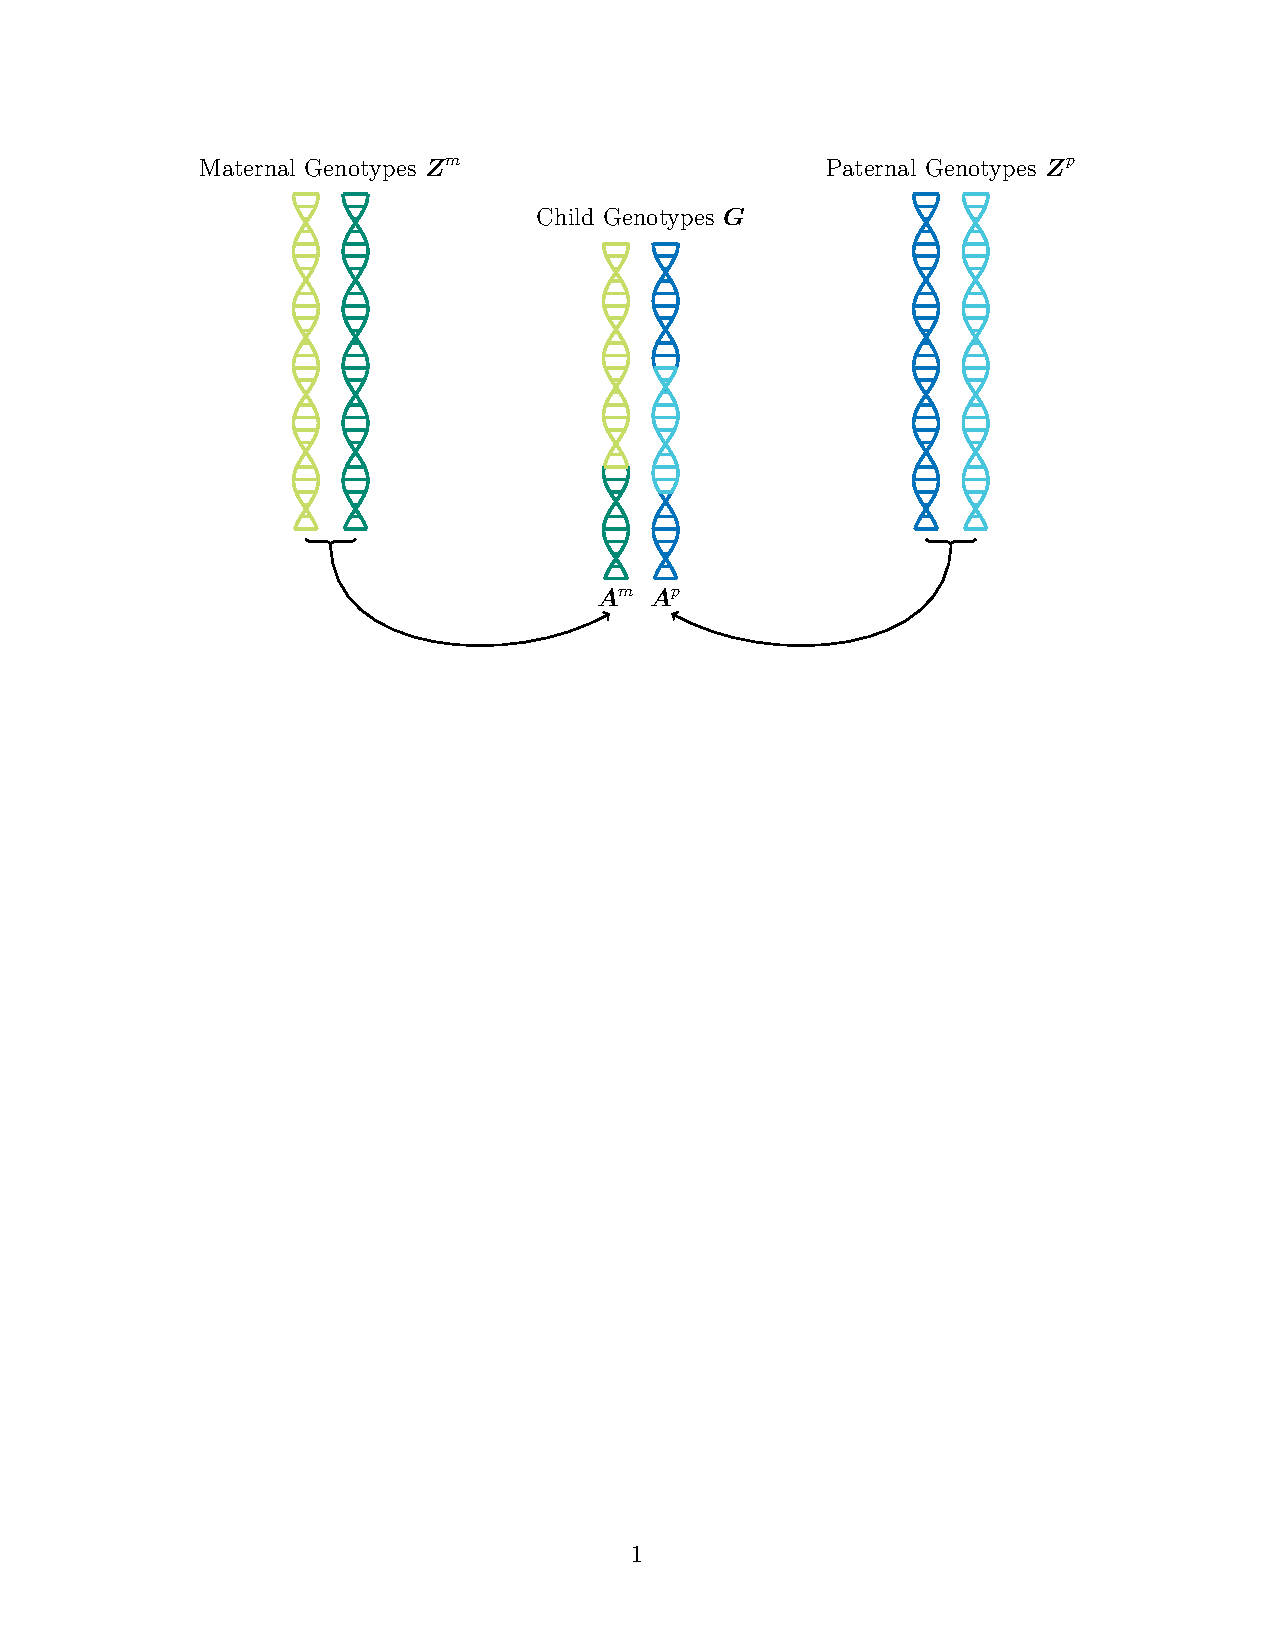
\includegraphics[clip, trim=3cm 16.5cm 3cm 0.5cm, width = 1\textwidth]{./figures/figures1.pdf} % trim by left botm right top
   \caption{\textbf{Schematic of a typical set of trio data and the meiosis process.} The transmission of alleles from heterozygous parents to the child motivate the randomized experiments to identify causal relationship between the child's phenotypes and genotypes. Recombination events may occur, marked as the adjacent dark and light colored pieces for the child's genotypes.}
   \label{fig:randomization}
\end{figure}


\begin{figure}[htbp] %  figure placement: here, top, bottom, or page
   \centering
   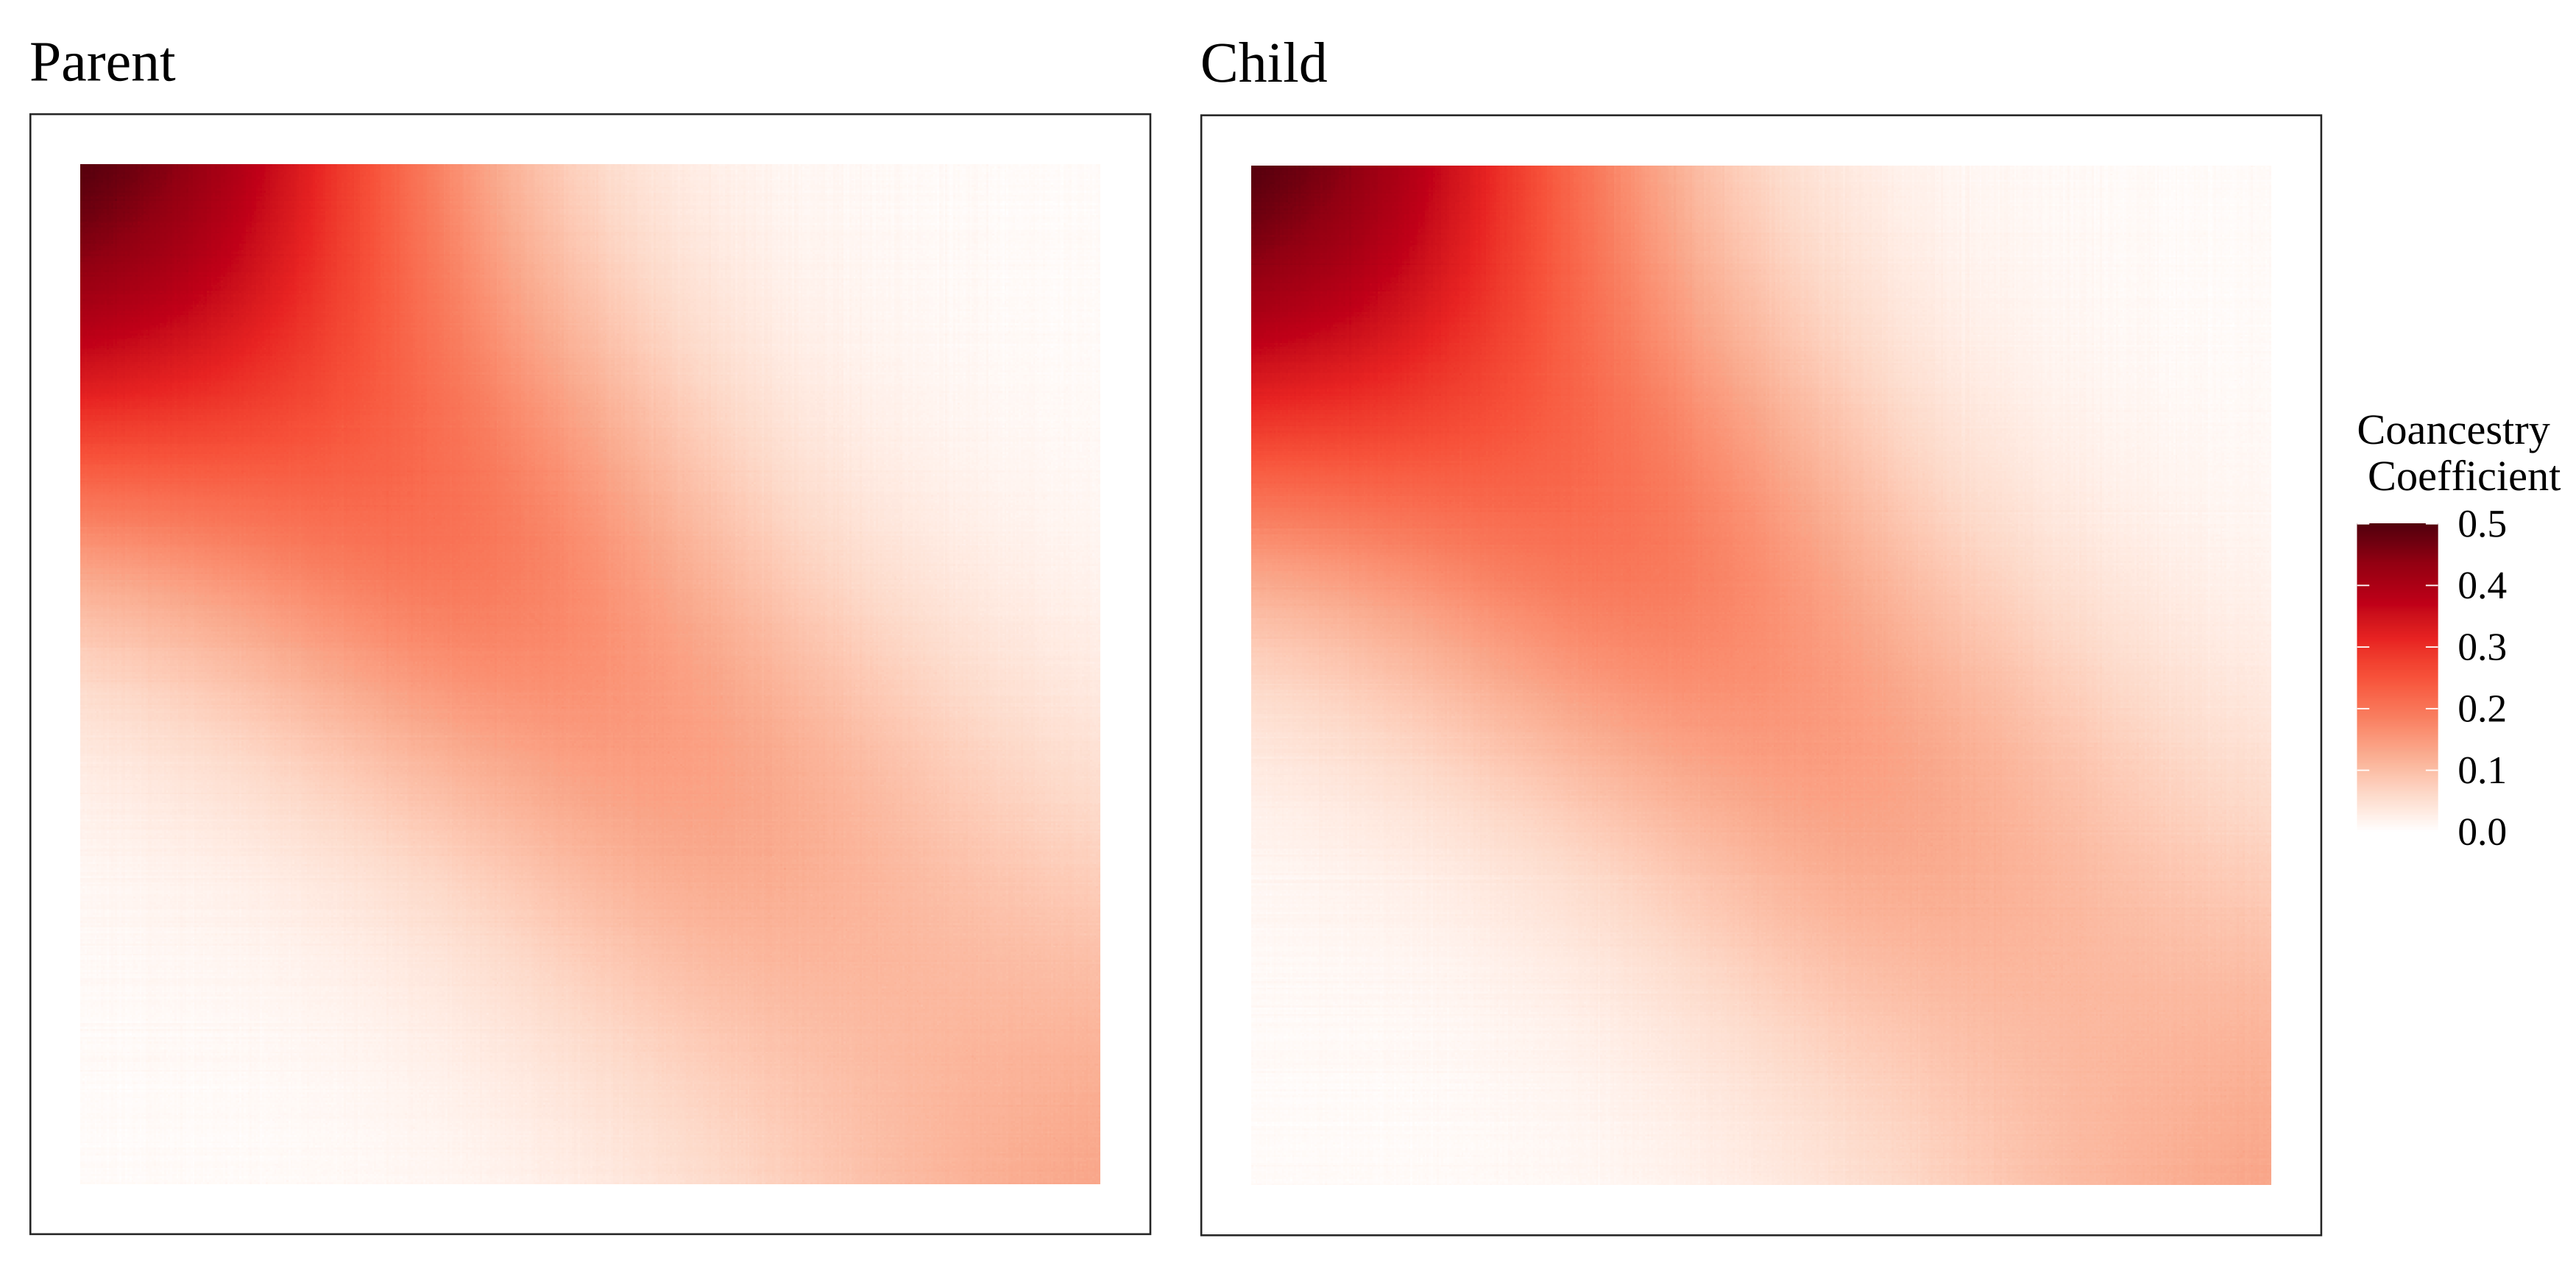
\includegraphics[clip, trim=0cm 0cm 0cm 0cm, width = 0.9\textwidth]{./figures/figures2.png} % trim by left botm right top
   \caption{\textbf{The co-ancestry coefficients between individuals among the structured population.} Along both x-axis and y-axis lined up the individuals, mothers for the left panel and children for the right panel. Each entry is a pair-wise coancestry coefficient calculated by \texttt{popkin} \citep{ochoa2021} for a simulated sample of 500 trios randomly drawn from the structured population. Here we presented a sample of 500 trios due to the limited figure size. Simulations throughout the paper with larger sample sizes share the same pattern of population structure and the same variability of coancestry coefficients with the overall $F_{ST}=0.2$.}
   \label{fig:pop_structure}
\end{figure}


\begin{figure}[htbp] %  figure placement: here, top, bottom, or page
   \centering
   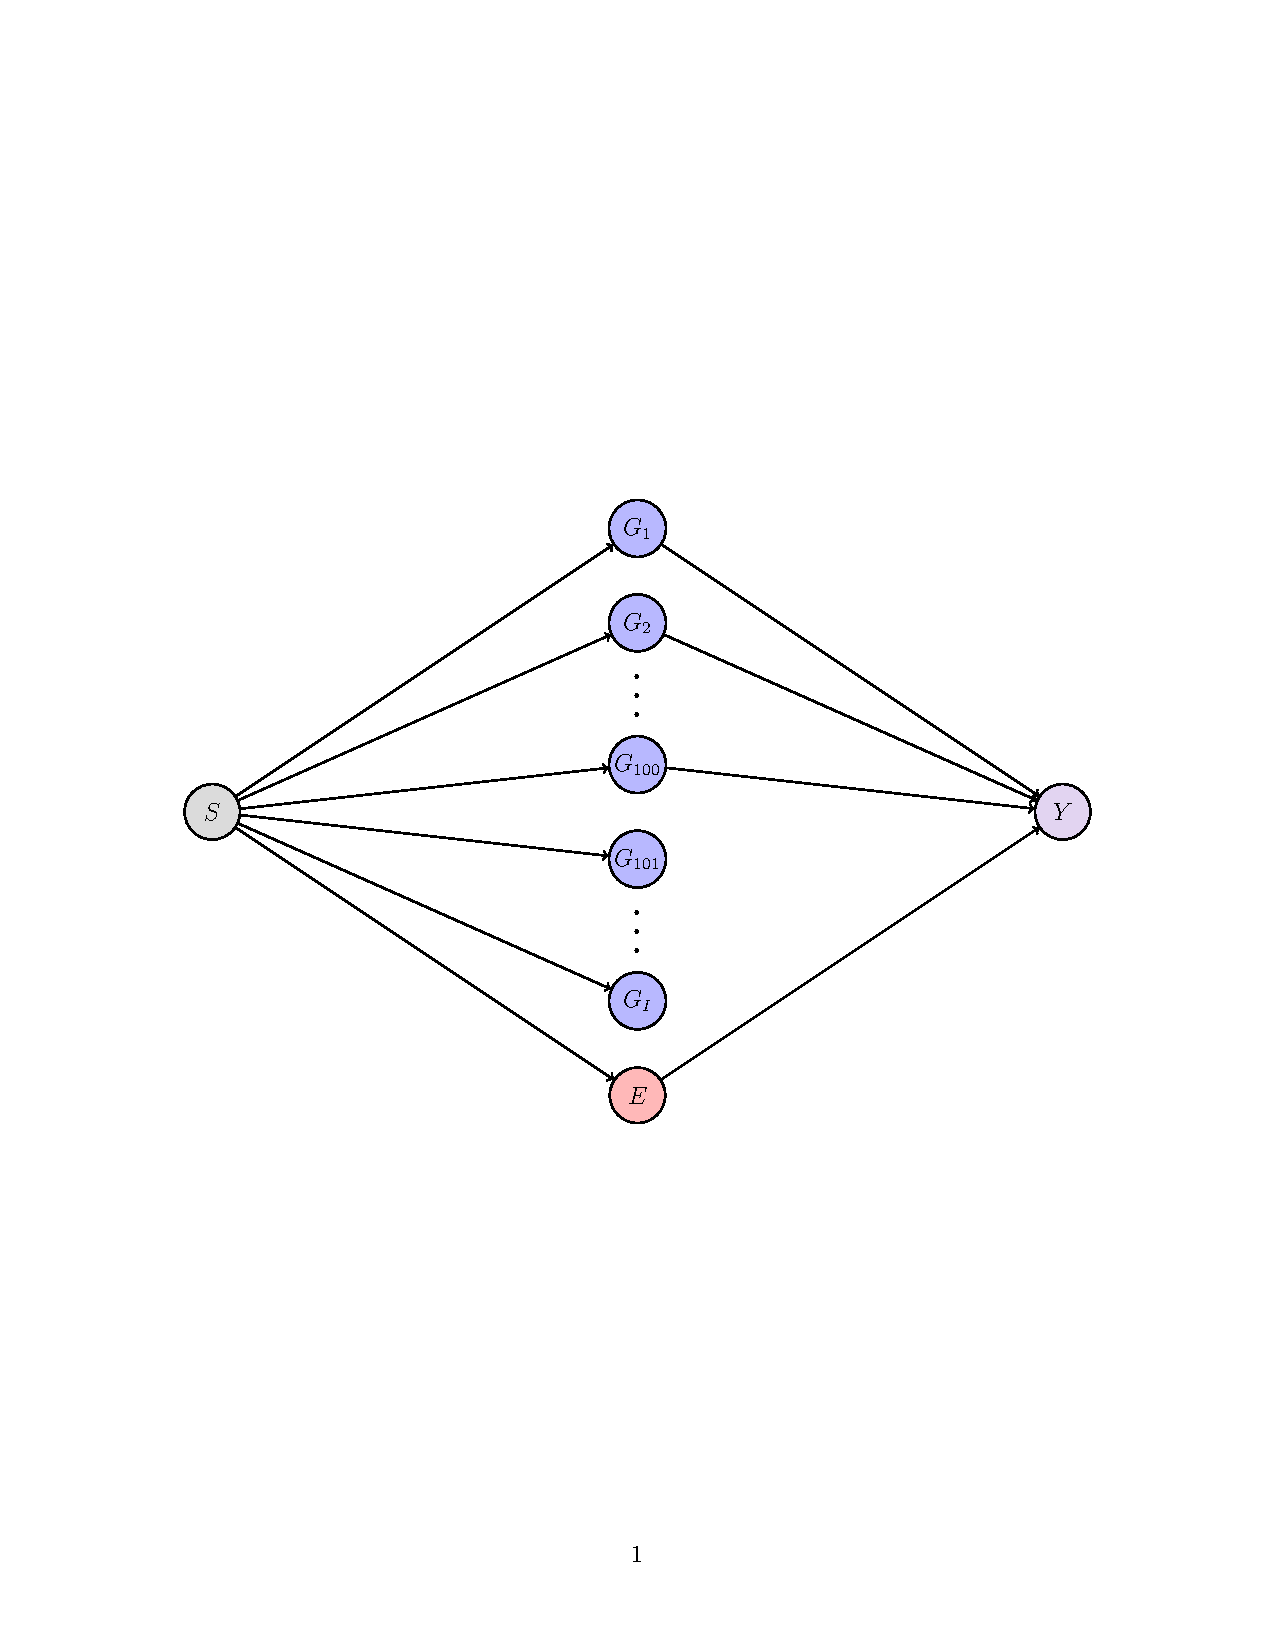
\includegraphics[clip, trim=3cm 8cm 3cm 8cm, width = 0.88\textwidth]{./figures/figures3.pdf} % trim by left botm right top
   \caption{\textbf{Schematic of the data simulation model.} The phenotype $Y$ is a function of 100 directly causal loci $(G_1, G_2, \hdots, G_{100})$ and a non-genetic factor $E$. The remaining loci $(G_{101}, G_{102}, \hdots, G_I)$ are not causal for $Y$. All non-genetic and genetic variables $(E, G_1, G_2, \hdots, G_I)$ are probabilistically dependent according to the population structure, represented by the variable $S$.}
   \label{fig:y_simulate}
\end{figure}


\begin{figure}
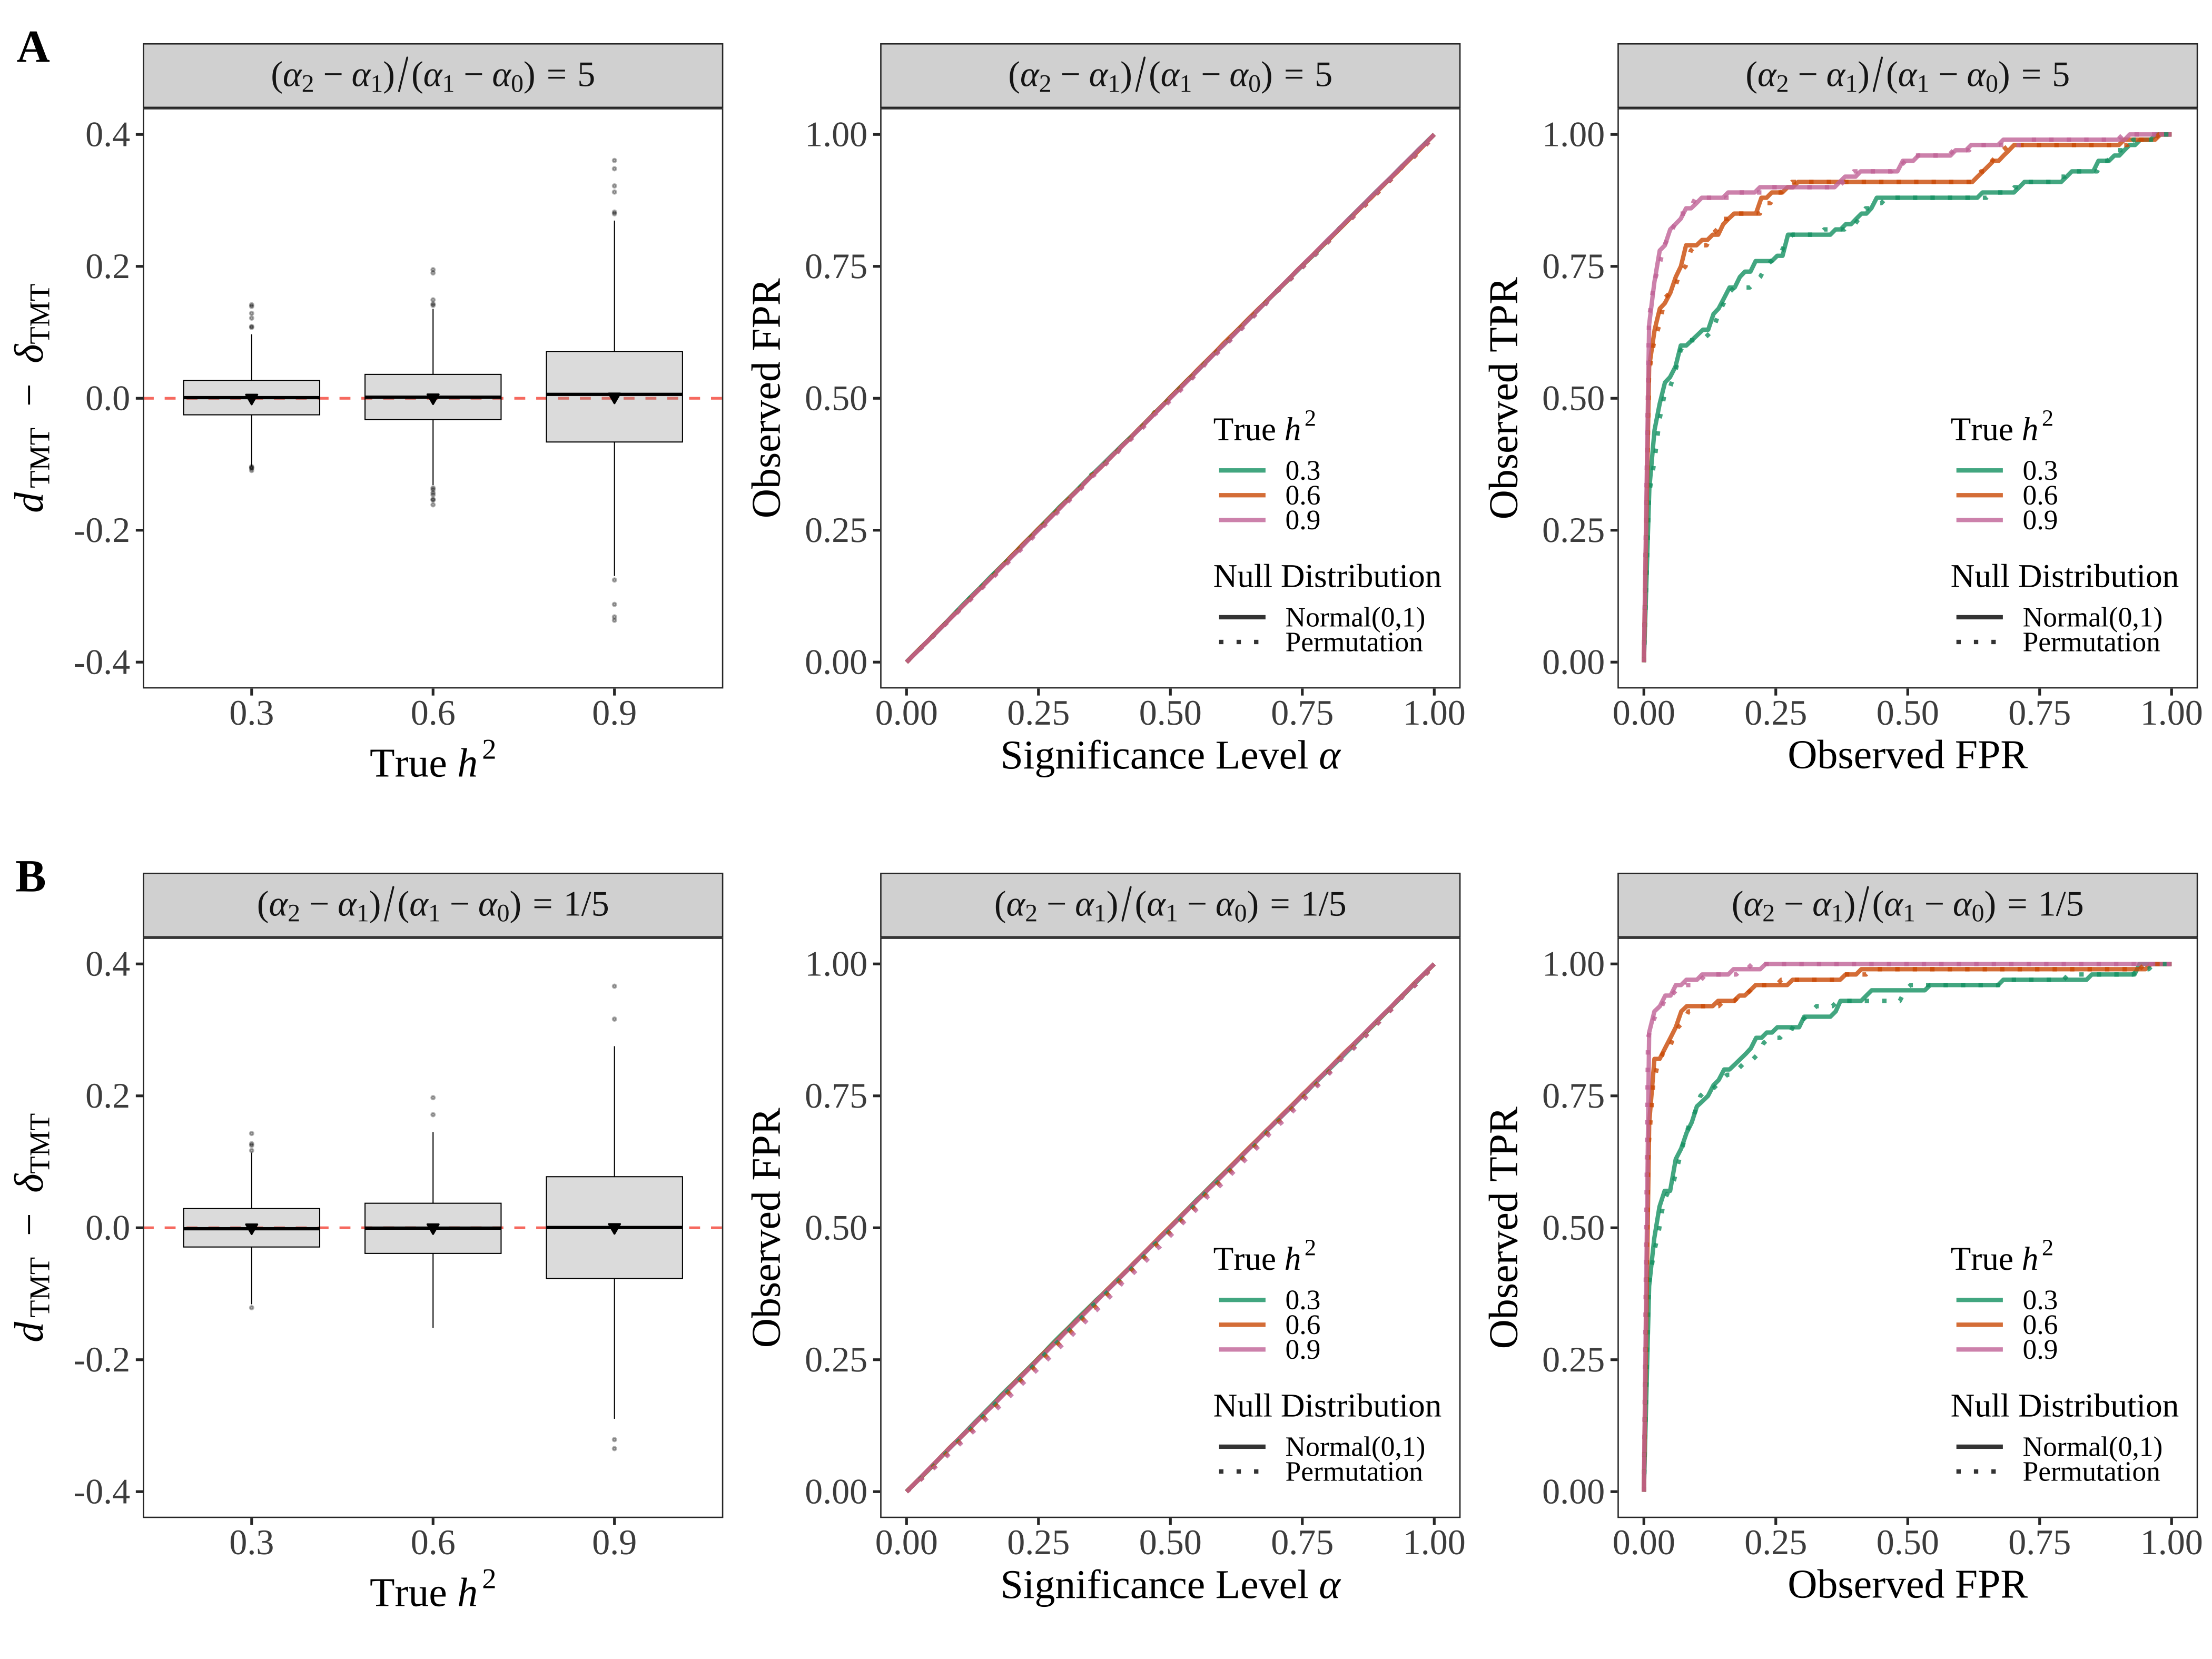
\includegraphics[clip, trim=0cm 2cm 0cm 0cm, width = 1\textwidth]{./figures/figures4.png} % trim by left botm right top
\caption{\textbf{The TMT delivers unbiased causal effect estimand $d_{\tmt}$, controls FPR at the desired significance level, and has reliable ROC curve across various levels of heritability $h^2$. (A)} Simulation results for $(\alpha_2-\alpha_1)/(\alpha_1-\alpha_0)=5$. \textbf{(B)} Simulation results for $(\alpha_2-\alpha_1)/(\alpha_1-\alpha_0)=1/5$. We followed \Cref{app:sim_trio_geno} to draw $5,000$ trios from an admixed population ($F_{ST}=0.2$) with $100,000$ SNPs and $100$ causal loci per individual. We simulated quantitative traits by following \Cref{app:sim_quant_trait}.}
\label{fig:tmt_various_parameters}
\end{figure}


\begin{figure}[htbp] %  figure placement: here, top, bottom, or page
   \centering
   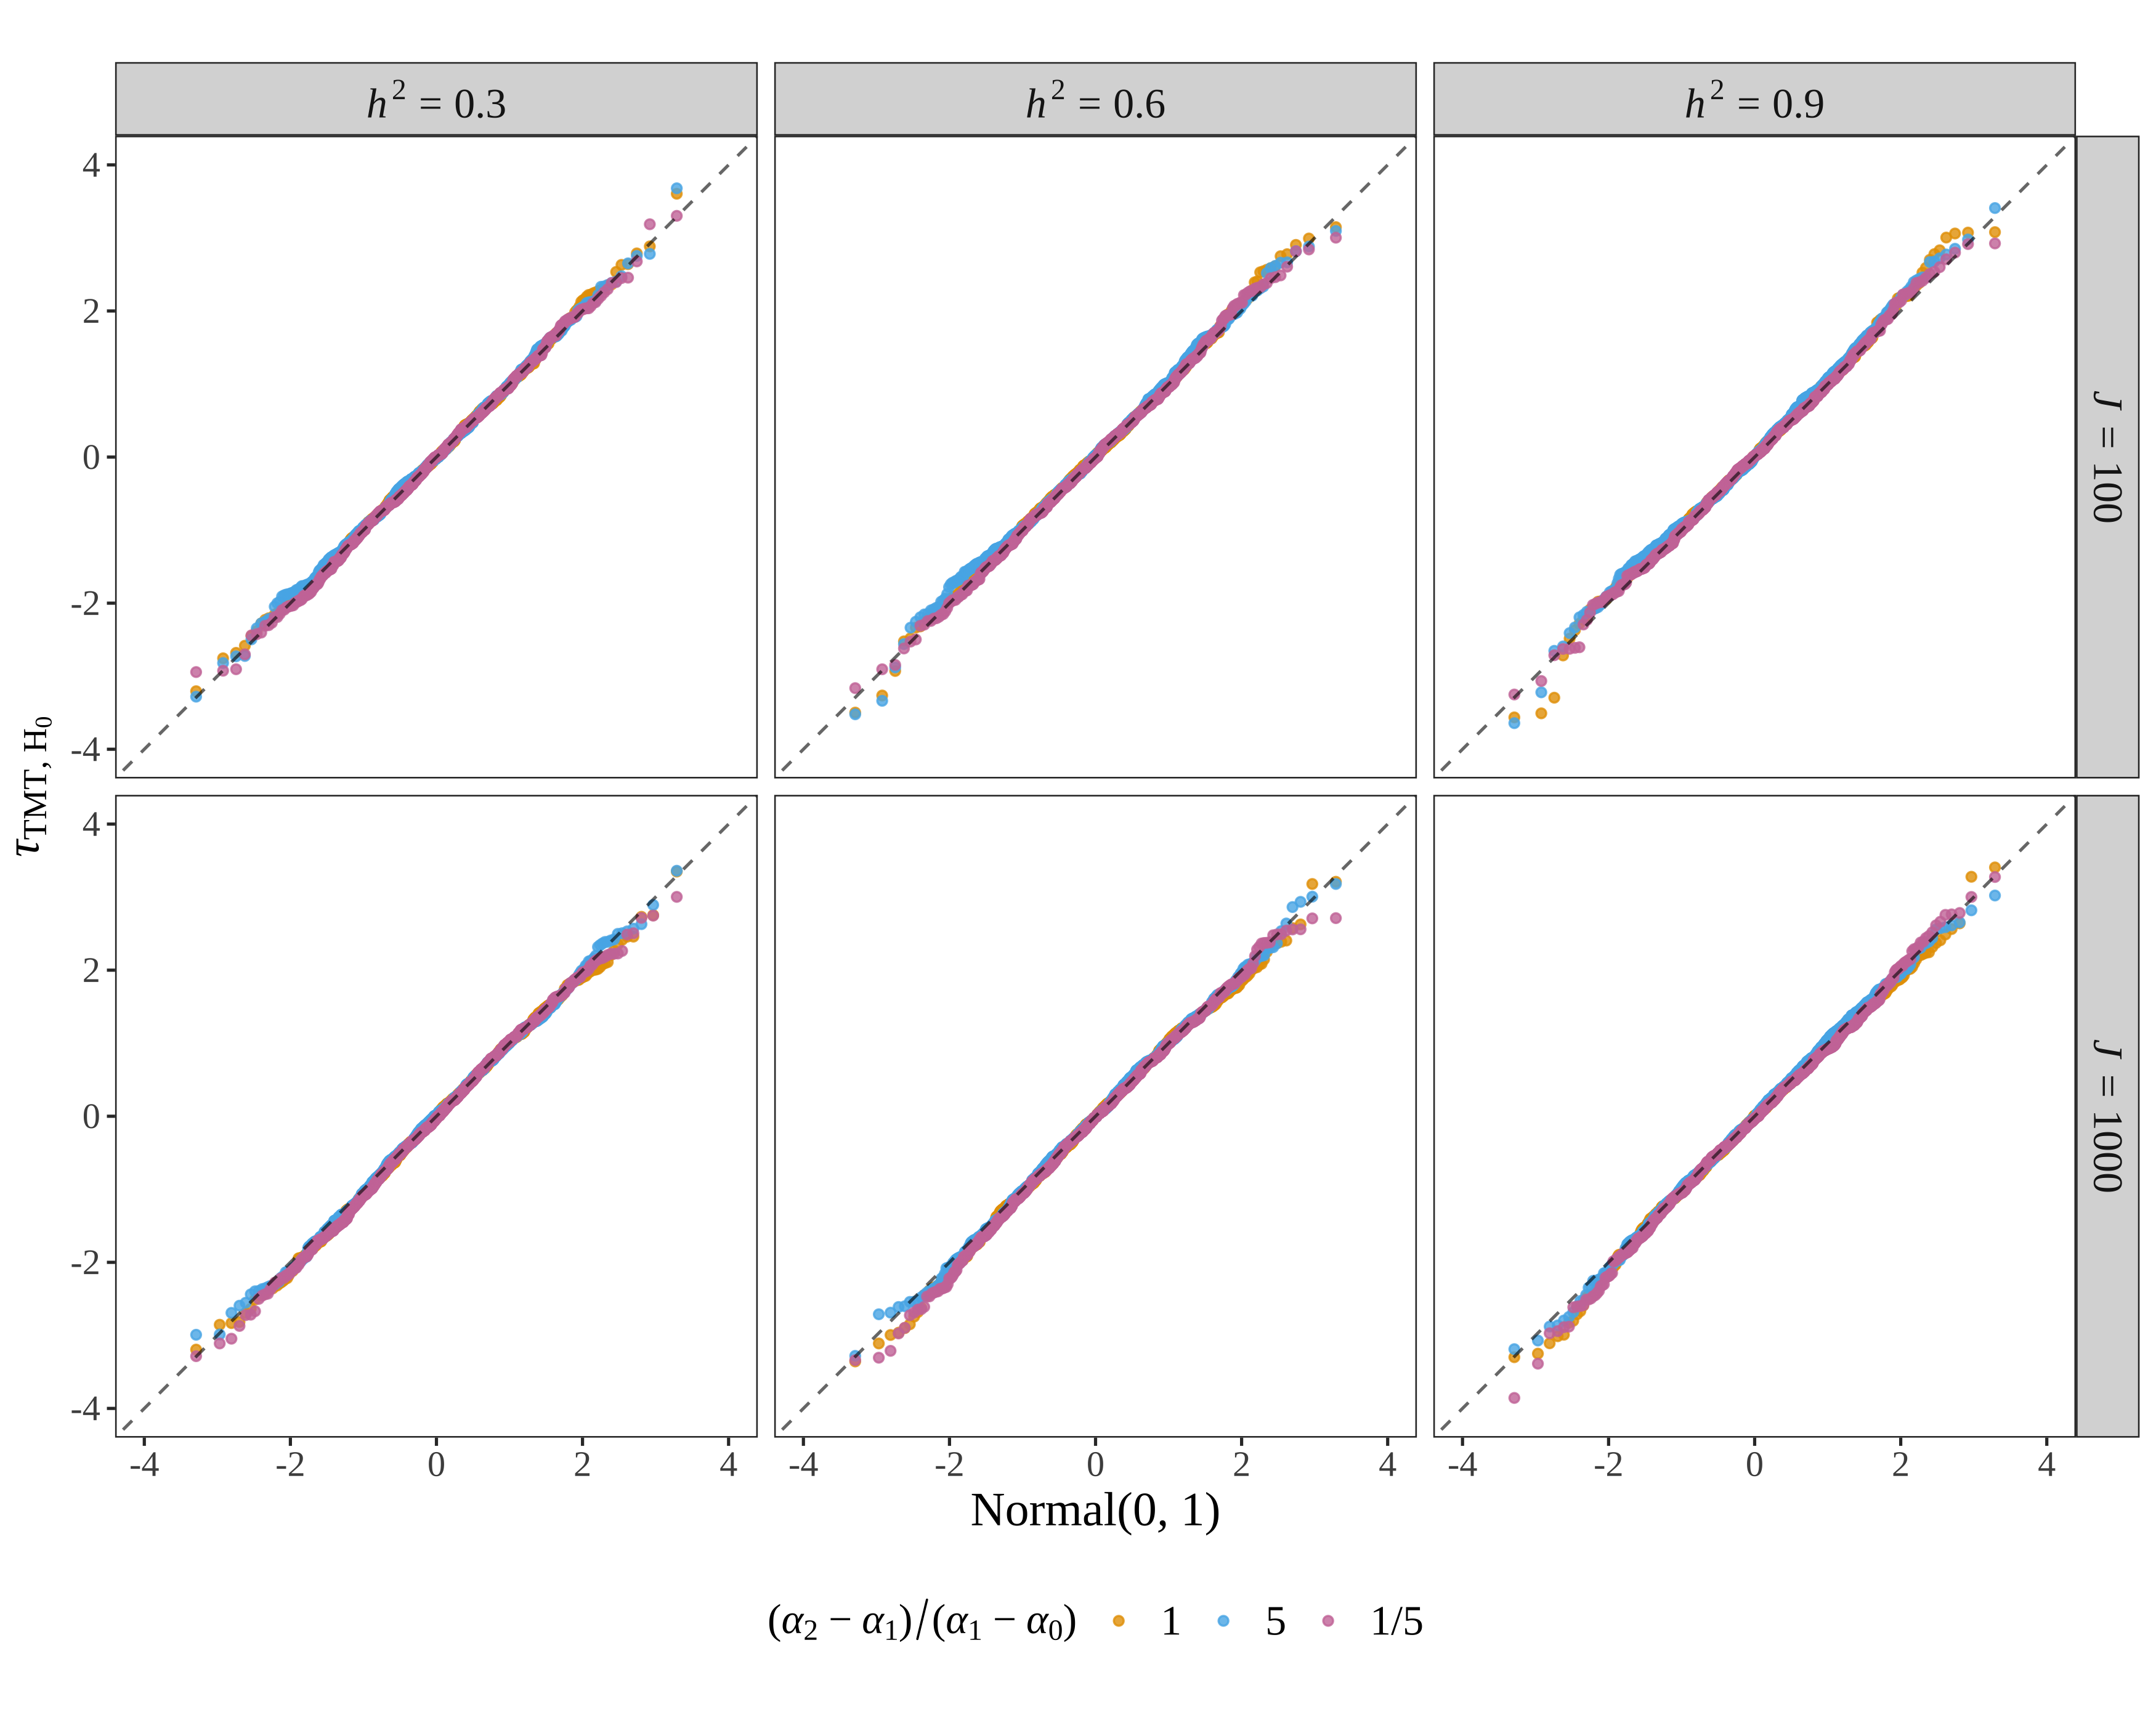
\includegraphics[clip, trim=0cm 0cm 0cm 0cm, width = 1\textwidth]{./figures/figures5.png} % trim by left botm right top
   \caption{\textbf{The Q-Q plot for the statistic $\tau_{\tmt}$ under null.} We followed \Cref{app:sim_trio_geno} to draw $100$ and $1,000$ trios from an admixed population ($F_{ST}=0.2$) with $100,000$ SNPs and $100$ causal loci per individual. The desired $h^2$ is 0.5. We simulated quantitative traits by following \Cref{app:sim_quant_trait}. For a randomly chosen causal locus, we conducted 1,000 permutations on trait values and calculated the statistic $\tau_{\tmt}$ per permutation to generate the observed null.}
   \label{fig:tmt_t_null}
\end{figure}


\begin{figure}
   \centering
   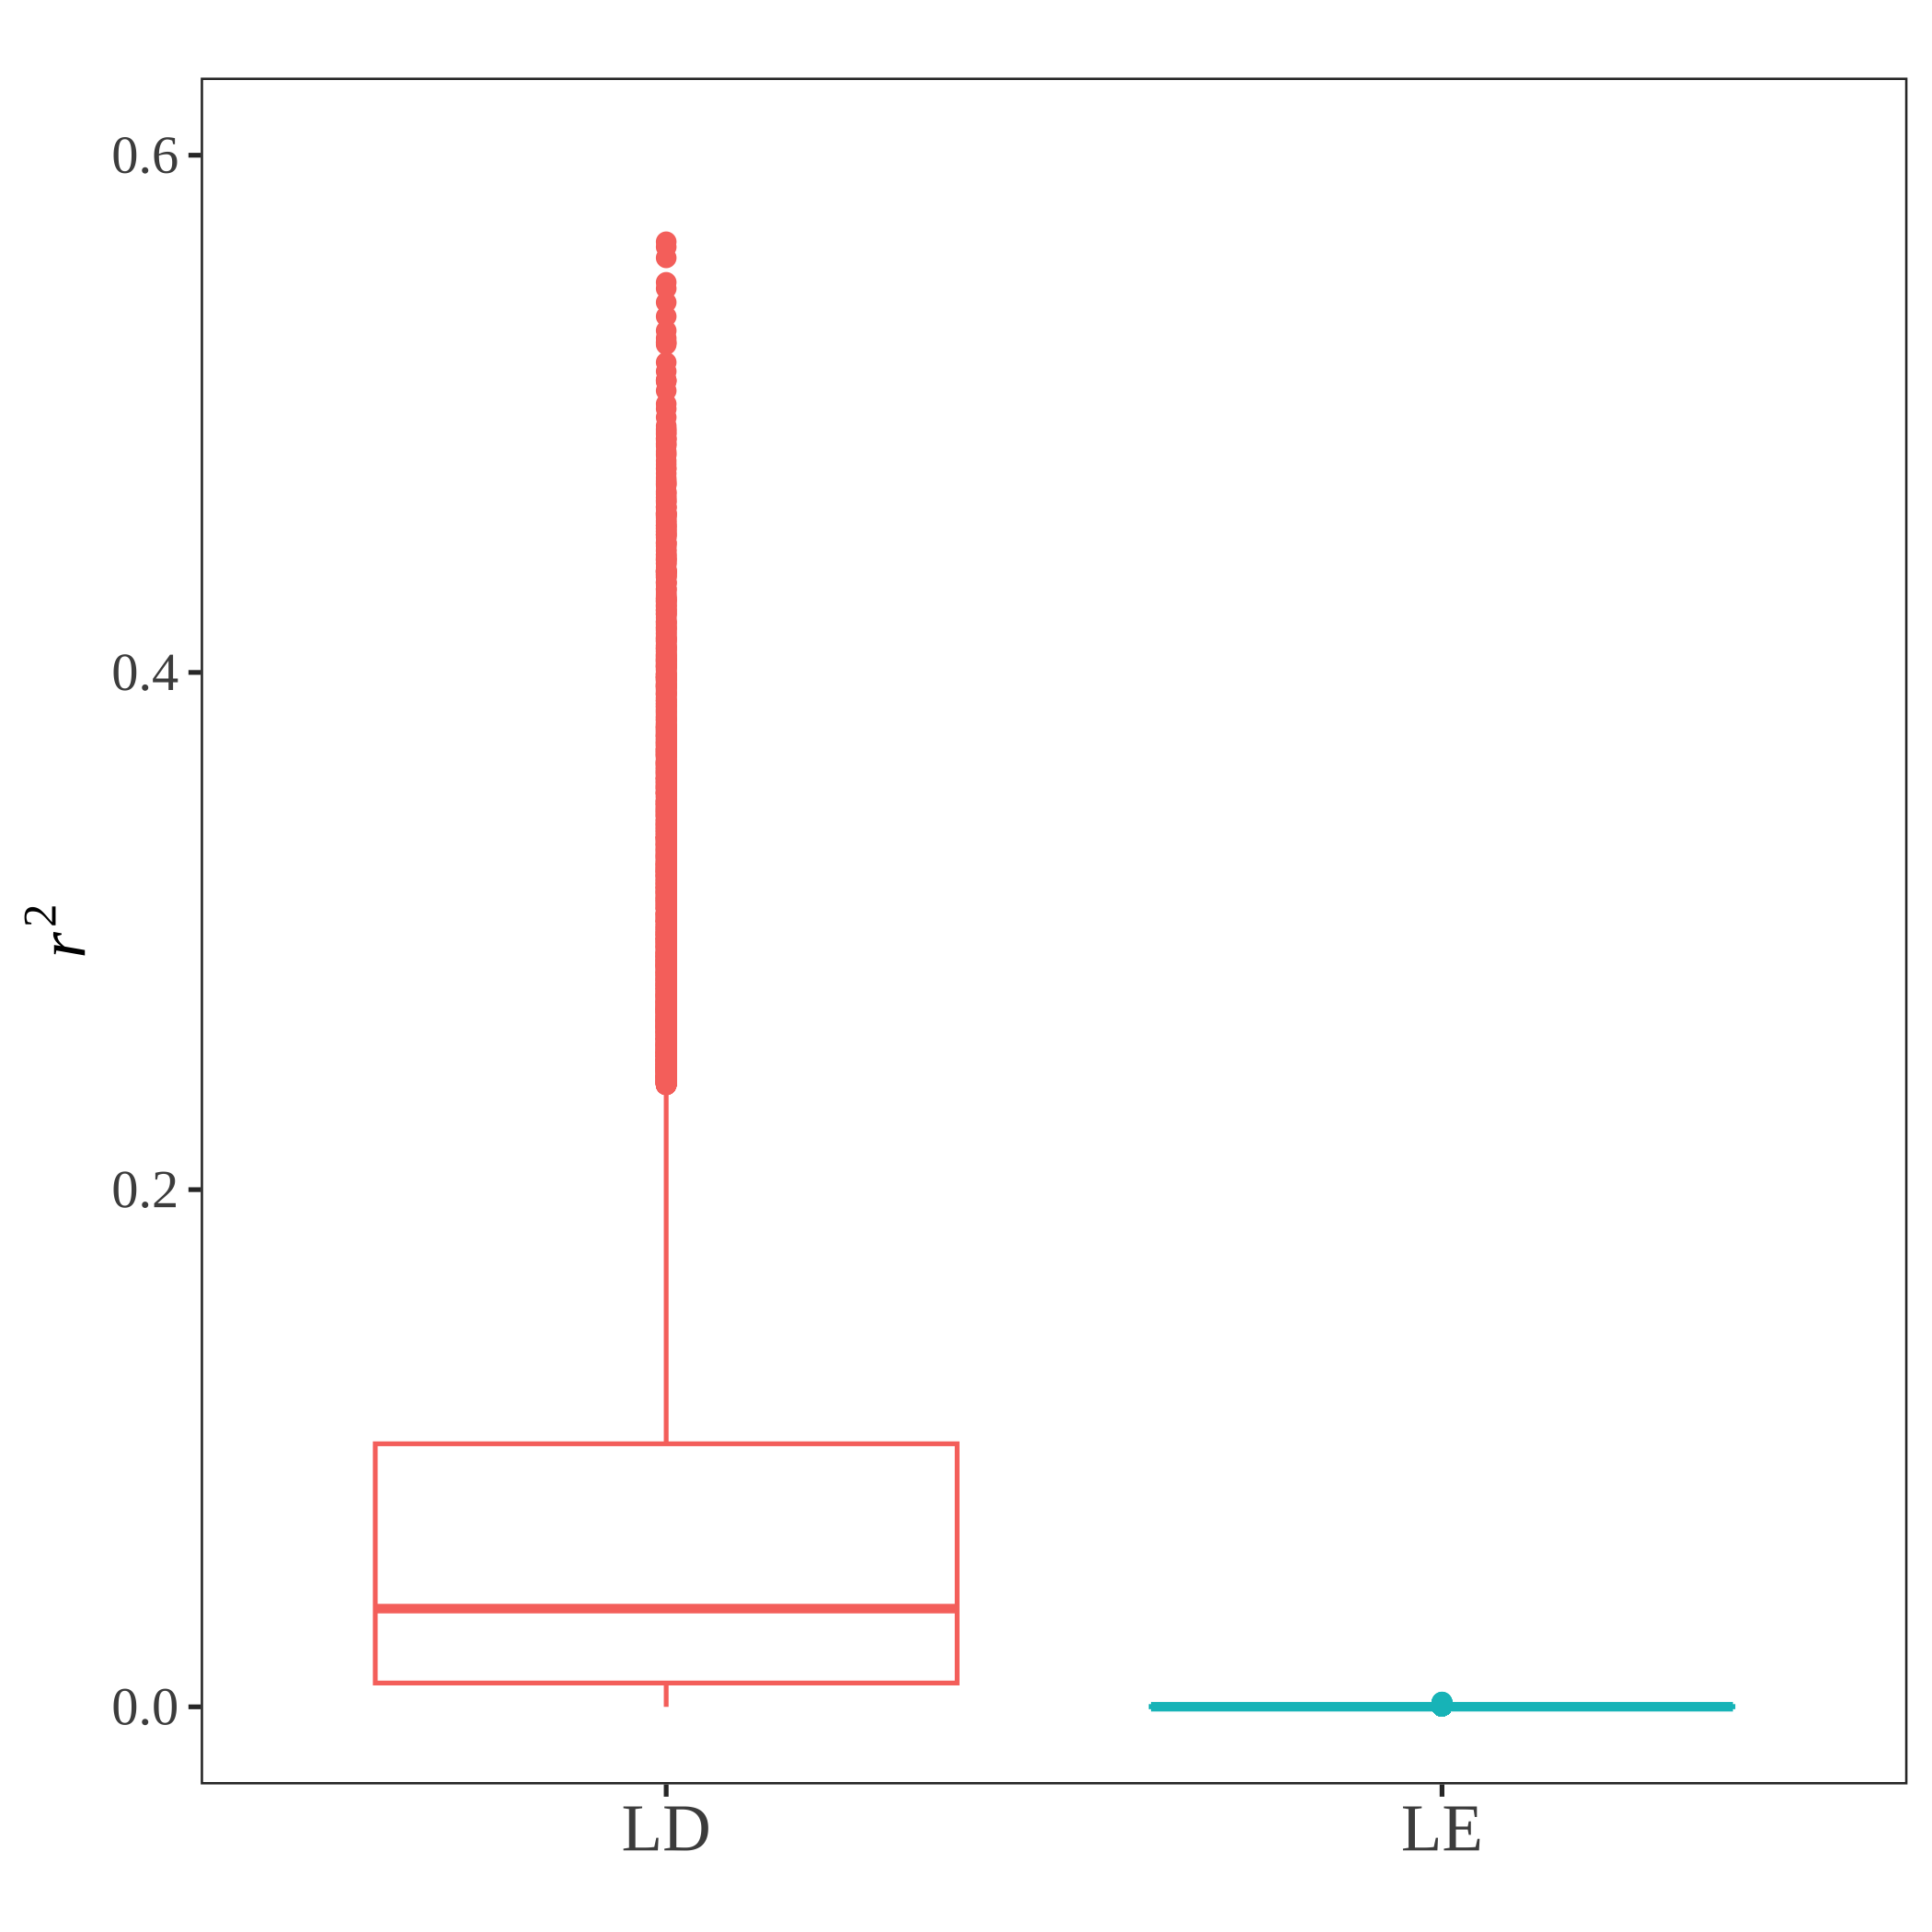
\includegraphics[clip, trim=0cm 0cm 0cm 0cm, width = 0.6\textwidth]{./figures/figures6.png} % trim by left botm right top
   \caption{\textbf{The distribution of $r^2$ between adjacent SNPs.} The $r^2$ values are shown for all pairs of adjacent SNPs for the simulated linkage-disequilibrium (LD) scenario and the linkage-equilibrium (LE) scenario after permutation.}
\label{fig:ld}
\end{figure}

\clearpage

\begin{figure}
   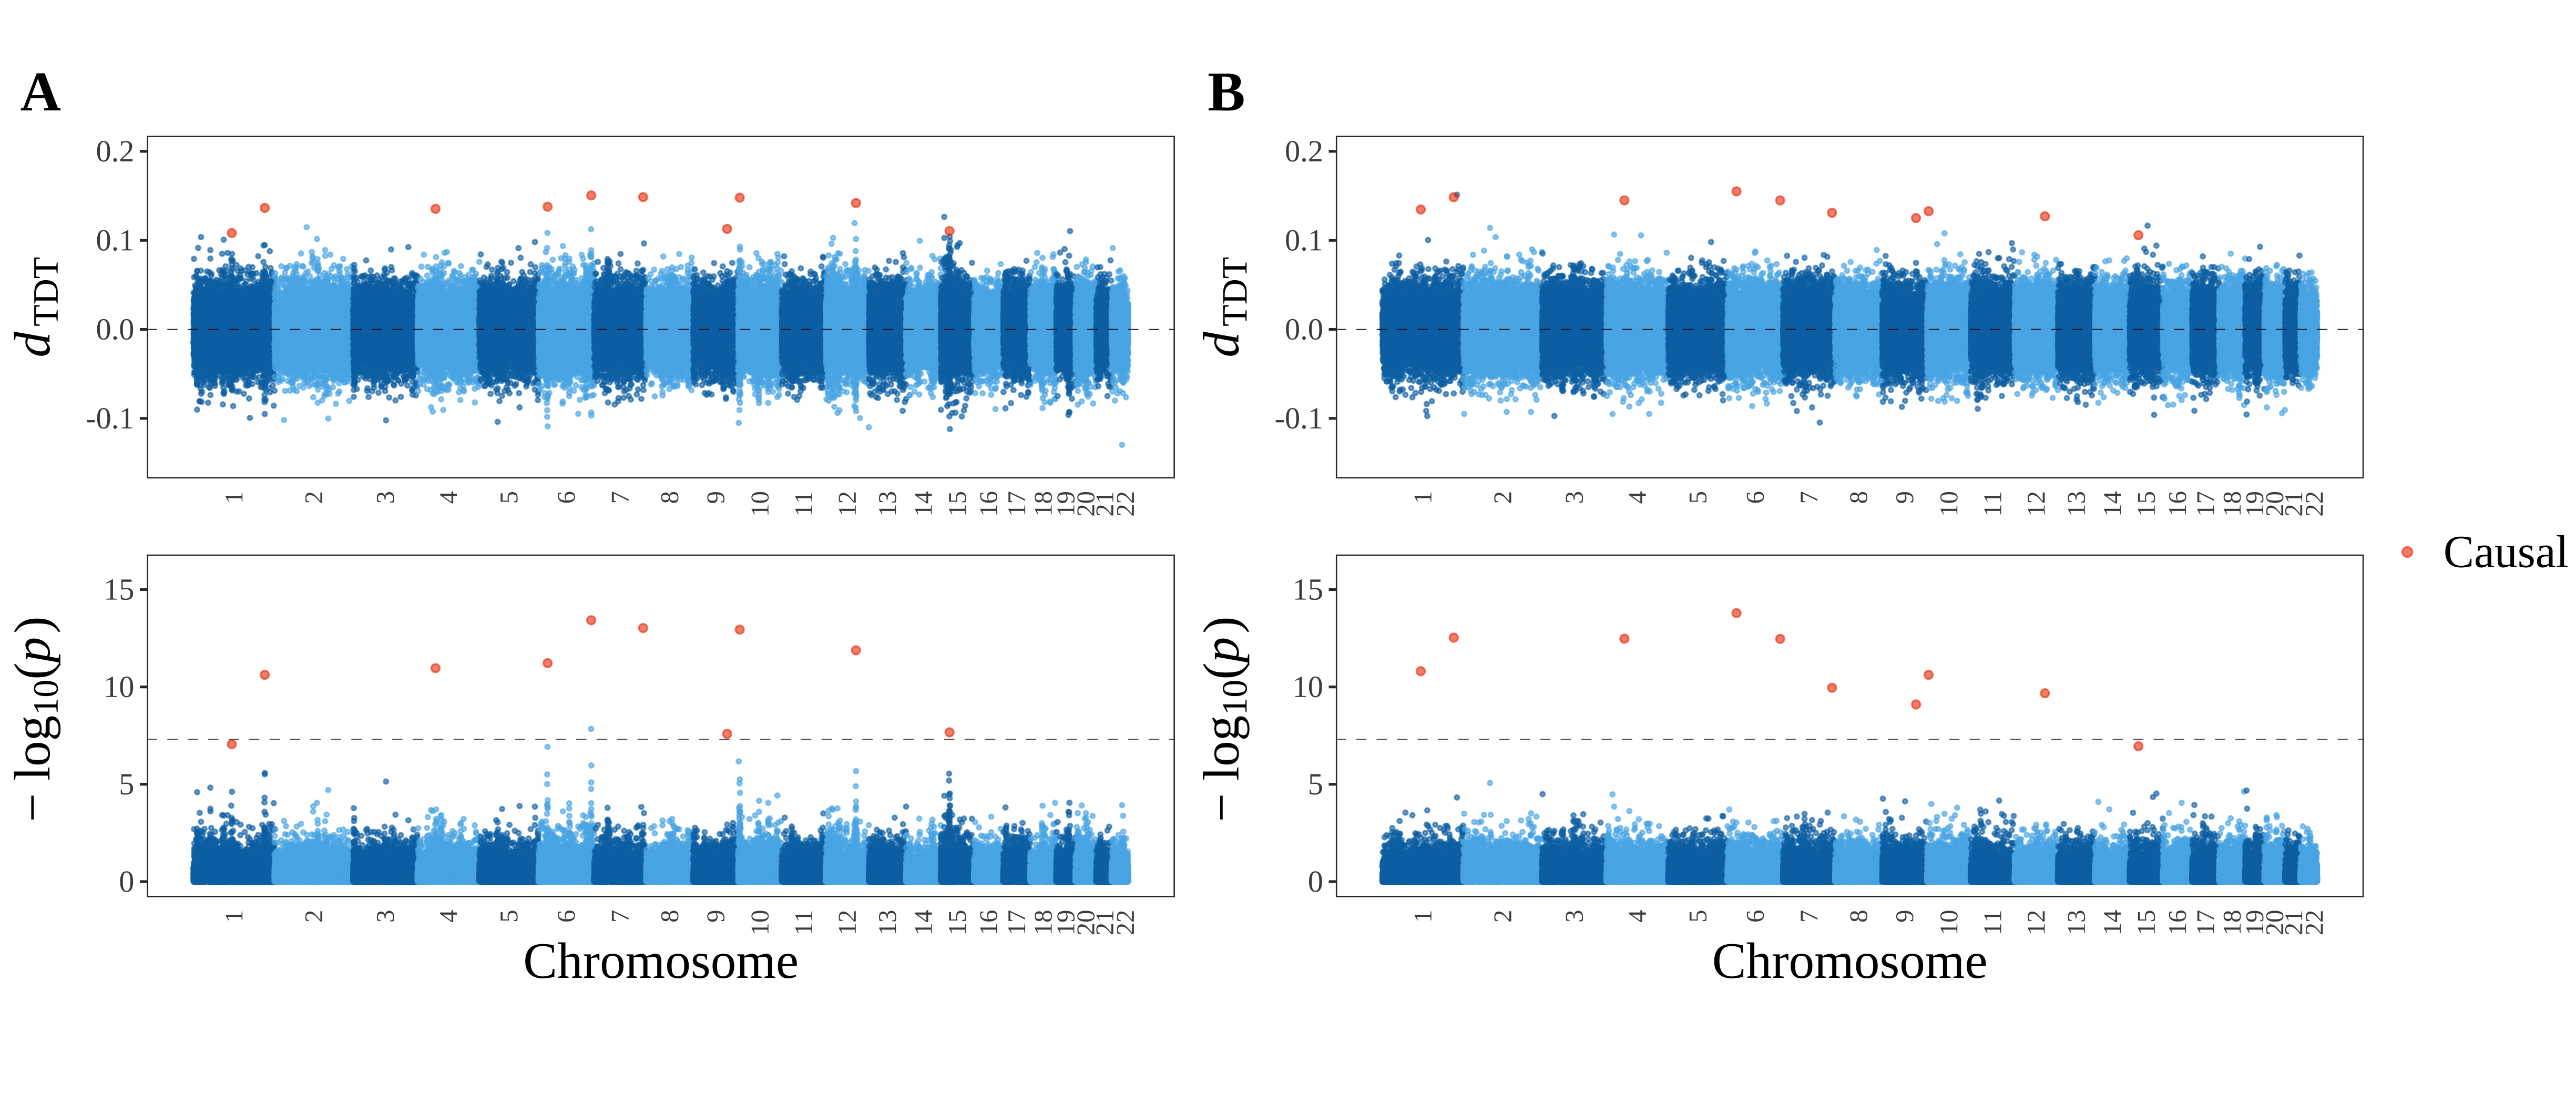
\includegraphics[clip, trim=0cm 0cm 0cm 0cm, width = 1\textwidth]{./figures/figures7.png} % trim by left botm right top
   \caption{\textbf{The genome-wide TDT profile for 2,500 affected-only trios.} \textbf{(A)} Randomization linkage scenario. \textbf{(B)} Independent randomization scenario, where the genotypes from (A) were independently permuted to remove the randomization linkage. Genotypes of 5,000 trios are simulated by \Cref{app:simulate_genetic_linkage}. For both scenarios, the top 2,500 children with the highest value of $\intercept+\sum_{i\in \cC}bG_{ij}+\epsilon_j$ are assigned as affected, setting the trait $Y_j=1$ and including in the TDT analysis. We draw $\epsilon_j$ from Normal($0,\sigma^2_e$), set $\intercept=100$, $\sigma^2_e=1$ and determine $b$ such that $\V\left(\sum_{i\in \cC}bG_{ij}\right)/\sigma^2_e=1$. The TDT profile is presented as $d_{\tdt}$ and $-\log_{10}$($p$) at 100,000 SNPs across 22 chromosomes simulated by \texttt{msprime}. The gray dashed line in the bottom panel is at $p$-value = $5\times 10^{-8}$, which is commonly used as a $p$-value threshold in GWAS.}
\label{fig:tdt_profile}
\end{figure} 

%\begin{figure}[htbp] %  figure placement: here, top, bottom, or page
%   \centering
%   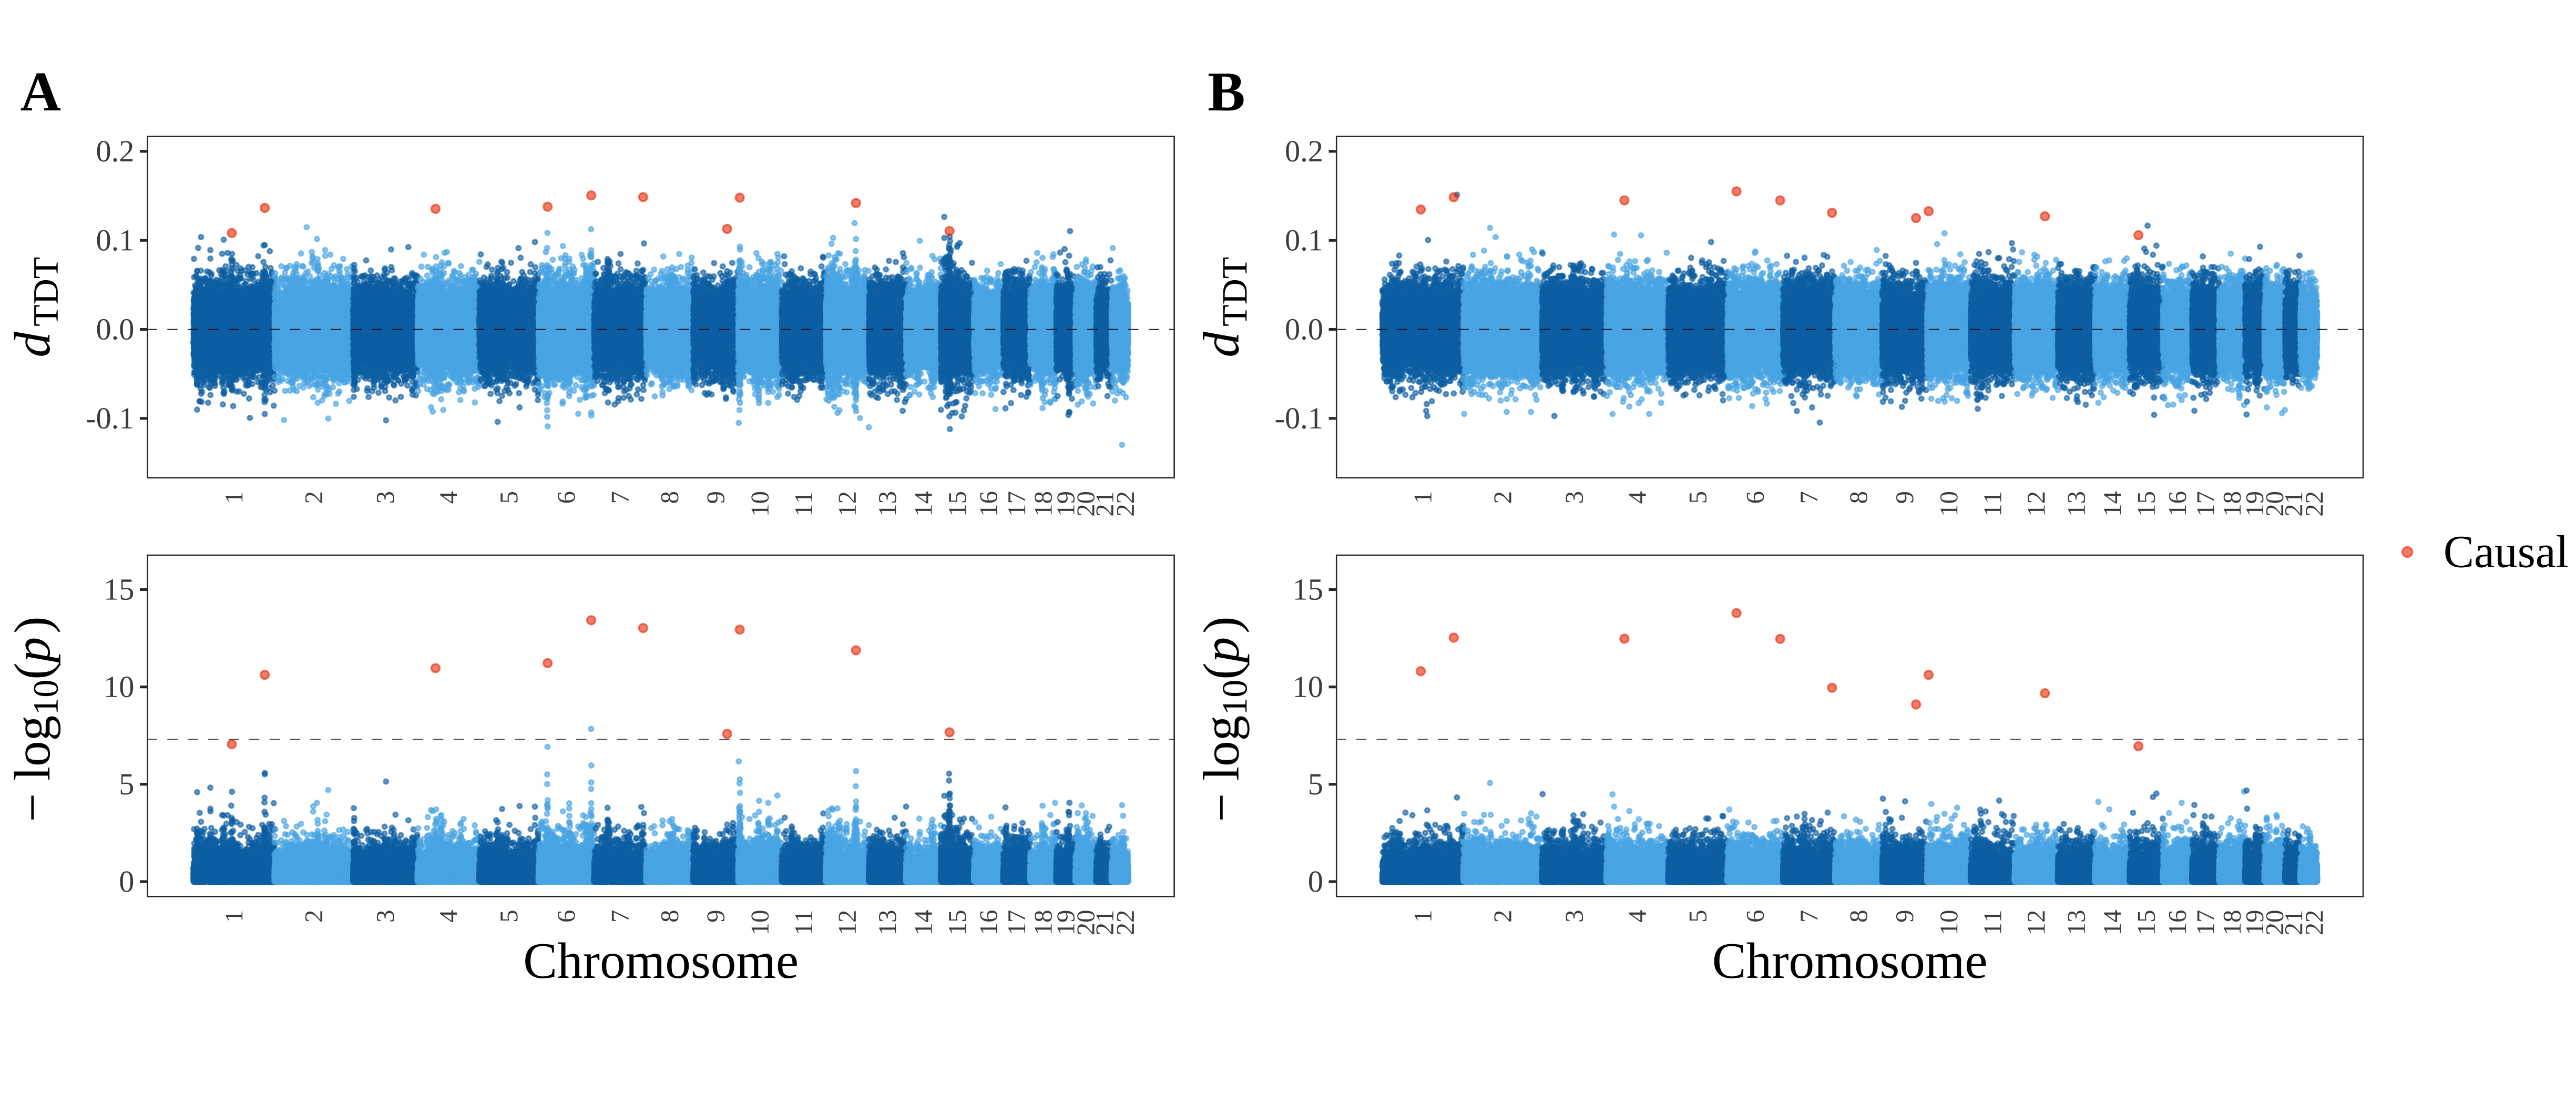
\includegraphics[clip, trim=0cm 10cm 0cm 0cm, width = 0.9\textwidth]{./figures/figures7.png} % trim by left botm right top
%   \caption{\textbf{Comparisons to established methods. (A)} FPR for binary traits. \textbf{(B)} The area under the ROC curve for binary traits. (A) displays results of a single round of simulation for 1,000 trios with 50,000 SNPs and 20 directly causal loci per individual. The desired $h^2$ is 0.5 while choosing other levels of desired $h^2$ produced similar results. Each box in (B) contains 100 simulations results.}
%   \label{fig:tdt_assoc}
%\end{figure}

%\begin{table}[htbp]
%  \centering
%  \caption{ \textbf{Frequently used mathematical notations.} }
%  \label{tab:term}
%  \begin{tabular}{ccp{4.1in}}
%    \hline
%    Symbol  & Sample Space & Definition\\
%    \hline
%    $G_{ij}$ & $\{0,1,2\}$ & Child $j$'s genotype at locus $i$. $G_{ij}=A_{ij}^m+A_{ij}^p$.  \\
%    $A_{ij}^m$ ($A_{ij}^p$) & $\{0,1\}$ & Child $j$'s haplotype from the maternal (paternal) side. $A_{ij}^m = A_{ij}^{mm}$ or $A_{ij}^{mp}$, $A_{ij}^p = A_{ij}^{pm}$ or $A_{ij}^{pp}$. \\
%    $Z_{ij}^m$ ($Z_{ij}^p$) & $\{0,1,2\}$ & The maternal (paternal) genotype at locus $i$ in trio $j$. $Z_{ij}^m=A_{ij}^{mm}+A_{ij}^{mp}$, $Z_{ij}^p=A_{ij}^{pm}+A_{ij}^{pp}$.  \\
%    $A_{ij}^{mm}$ ($A_{ij}^{pm}$) & $\{0,1\}$ & Mother (Father) $j$'s haplotype at locus $i$ from their maternal side. \\
%    $A_{ij}^{mp}$ ($A_{ij}^{pp}$) & $\{0,1\}$ & Mother (Father) $j$'s haplotype at locus $i$ from their paternal side. \\
%    $Y_{j}$ & $\mathbb{R}$, $\mathbb{N}$, or $\{0,1\}$ & Child $j$'s phenotype for continuous, counts, or binary trait values. \\
%    \hline
%  \end{tabular}
%\end{table}

\end{document}